\chapter{Pattern Recognition and Implementation}

% **************************** Define Graphics Path **************************

\epstopdfsetup{outdir=Chapter4/Figs/PDF/}
\ifpdf
    \graphicspath{{Chapter4/Figs/Raster/}{Chapter4/Figs/PDF/}{Chapter4/Figs/}}
\else
    \graphicspath{{Chapter4/Figs/Vector/}{Chapter4/Figs/}}
\fi


\section{Implementing the Color Space}\label{sec:ImplementingTheColorSpace}

Appendix C outlines the practical algorithm which implements the techniques developed in the previous chapters, taking account of the phone characteristics. 
The resulting algorithm produces the image in the rotated color-space along with a classified image, which takes four values relating to the probability that the pixel value is in the target color region.  

%\section{Fingertip Model}\label{sec:FingertipModel}
%
%We need an appropriate finger model so we can accurately align points on the fingertip between successive images in the video stream. We need to do this because otherwise, any difference between the frames will be overwhelmed by physical movement of the digit rather than movement of the blood inside the digit. For this reason, we target the most stable portion of the finger: the nail.
%
%A digit has two joints and three segments: the distal, the middle, and the proximal. Each segment is roughly approximated by a rectangle, and the length of each section approximately following a 2-3-5 ratio, with lengths counting from distal to proximal, and where 1 is the $\frac{3}{4}$ width of the middle segment. Our finger model then comprises of the lengths and widths of each segment, the positions of the joints (i.e. {\tiny {\tiny }}the knuckles) between each segment, the position of the tip, and a position in the model marking the point at which the digit goes out of frame.
%
%Given the width of the middle segment, we can then have an initial guess that the length of the distal segment is 1.5 times the initial width, the middle is 2.25 times that, and the proximal is 3.75 times that. Additionally, the center of the nail feature is not in the center of the distal segment, but a half unit (in our model units) away from the tip. The model can be laid out in units relative to the width of the digit.

\section{The Finger Shape Detection Algorithm}\label{sec:FingerShapeDetectionAlgorithm}


\subsection{Finding the Frame Orientation}\label{sec:FindingTheFrameOrientation}
The first step of the algorithm is to detect which of the four frame edges the finger is entering from. This is done simply by finding the longest on-object path running along the frame sides. So, the algorithm starts by looking down the pixels on a frame side; when it locates a high-quaternary value (Section \ref{sec:QuaternaryPixelClassification}), it uses the Hurdle method (Section \ref{sec:HurdleMethod}) to find the longest path in that direction starting from that point. It continues around all four sides; the longest path found by the Hurdle algorithm is assumed to correspond to the finger entering the frame. From this, we set a frame orientation, which is the angle necessary to rotate the image such that the finger will be entering the frame from the left, and we set a direction vector pointing inwards from the frame edge found.

\subsection{Finding the End of the Finger Shape}\label{sec:FindingTheEndOfTheFingerShape}
Taking the longest Hurdle path on the frame edge found above, we take the middle point on that path and start a 'Run-Reach' algorithm in the direction found previously from that point. The Run-Reach algorithm proceeds as follows:

It finds a Hurdle path in the primary direction, i.e. perpendicularly away from the frame edge. At the end of the Hurdle path, it finds the Hurdle paths in the two perpendicular directions to its primary direction, i.e. parallel to the frame edge. It then finds the midpoint between the ends of the Hurdle path, and then uses that to start a new Hurdle path in its primary direction. The algorithm continues in this way until the end of the finger is found, as seen in Figure \ref{fig:FindingTheTip}.

\begin{figure}[h!]
  \centering
    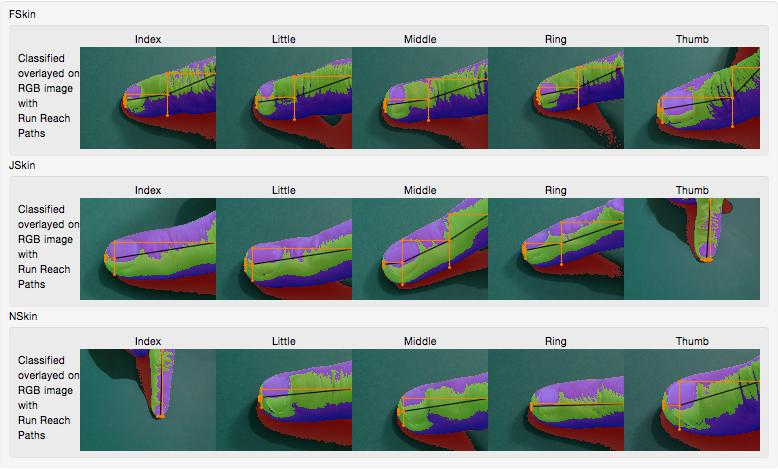
\includegraphics[width=0.95\textwidth]{Chapter4/Figs/FindingTheTip.jpg}
    \caption{Finding the End of the Finger Shape}\label{fig:FindingTheTip}
\end{figure}



\subsection{Filament Fill the Finger}\label{sec:FilamentFillTheFinger}
The center points found by the Run-Reach method above form a path on the finger. This is the path given to the Filament Fill method described in Section \ref{sec:FilamentFill}. We now have a set of edge points on the digit. These edge points also have a top and bottom correspondence which, although they're not perpendicularly-opposite points on the finger, they do allow for a midpoint on the digit to be found. This can be seen in Figure~\ref{fig:FillamentFill}.

\subsection{Exclude Secondary Frame Edge and Fingertip Points }\label{sec:ExcludeSecondaryFrameEdgePointsAndFingertipPoints}
We need to exclude from the calculation of the midpoints values which are near the tip, and values where one of the edge points touches a frame edge. This is because values toward the tip --- given that the finger is not necessarily perfectly horizontally-aligned --- give unreliable midpoint values because the Run-Reach path corresponds to shorter and shorter chords on a circle. Values where one of the edge points touches a frame edge, more likely than not, do not correspond to the edge of the digit, but are simply where the digit exits the frame (for example, JSkin Middle in Figure \ref{fig:ExcludedEdgePointsAndMidlineFit}).

\begin{figure}[h!]
  \centering
    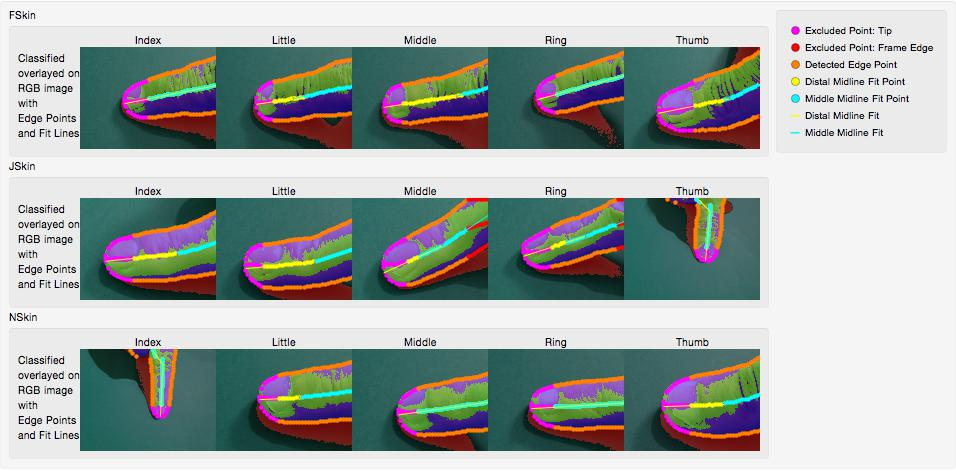
\includegraphics[width=0.95\textwidth]{Chapter4/Figs/ExcludedEdgePointsAndMidlineFit.jpg}
    \caption{Excluded Secondary Frame Edge Points and Fingertip Points, with the fit to the midline points returned by the Kink Fit algorithm.}\label{fig:ExcludedEdgePointsAndMidlineFit}
\end{figure}

To estimate which pairs of edge points correspond to points on the tip, the algorithm finds the length of the Hurdle path for all corresponding bottom-edge to top-edge points. These values are then sorted into ascending order, and then the 'Mean-Median' is taken (Section \ref{sec:MeanMedian}), ensuring that the average is not affected by extreme values. The tolerance is determined by the algorithm by looking at the difference at the low and high ends of the $66\%$ range used by the Mean-Median.

\subsection{Kink Fit to the Finger}\label{sec:KinkFitToTheFinger}
We now have a set of reliable points at the midpoint of the finger. Because the finger is articulated, it is reasonable to assume that it may well be bent. We're interested in the action of the finger being pressed on a surface --- as a result, the finger is expected to be articulated at the distal-middle joint, but is otherwise straight. We wish to fit a function which consists of two straight-line segments to the set of reliable middle points. The fit was found using the 'Kink Fit' algorithm described in Section \ref{sec:KinkFitMethod}.

The Kink Fit algorithm takes a set of points where the first component is assumed to be the independent variable and the second component to be the dependent variable. However, because we haven't assumed that the finger comes into the frame from any particular direction, this can be problematic if, say, the finger comes through from the top or bottom of the frame, then the components would be in the wrong order for the Kink Fit algorithm to work. This is easily rectified by simply rotating the points into a standard orientation as if the finger is coming in from the left side of the frame. The extra computational effort is minimal because the number of points is small. Performing the Kink Fit algorithm returns a set of three points, which can then be rotated back to the original orientation.

In practice, however, the Kink Fit algorithm accepts the full set of midline points and a vector of pointers to the reliable values within that set. This allows the Kink Fit algorithm to extend out the end points of the line to the edges of the digit. Were this not the case, the end points returned would lie somewhere within the digit corresponding with the first and last reliable midline points. The result can be seen in Figure \ref{fig:ExcludedEdgePointsAndMidlineFit}.

\subsection{Parallel Lines Fit}\label{sec:ParallelLinesFit}
Our model of a finger assumes that the edges are parallel to each other. Since we have a line which runs through the center of the finger, we can now calculate the distance of the edge points to that line. These distances can be classified as good edge points if they're parallel to the central line. Whether they are parallel is determined by finding the Mean-Median distance from the central line to the edge points using a $50\%$ interval in the distal portion, because it is expected that up to half the points may be in the distal segment, maybe on the tip, and a $75\%$ confidence interval in the middle segment, because we expect fewer than $\frac{1}{4}$ of the edge points to be anomalies. The points are then classified as good if they are of Mean-Median distance from the central line. It should be noted that we consider both the top and bottom edges when calculating the Mean-Median distance. This technique successfully removes anomalies which are not parallel to the central line.

There is one final step: the points which are classified as good edge points are used to find a linear fit which is parallel to the central line. Finally, the width of the distal and the middle segments is calculated by finding the distance between these parallel lines. This can be seen in Figure \ref{fig:ParallelFit}.

\begin{figure}[h!]
  \centering
    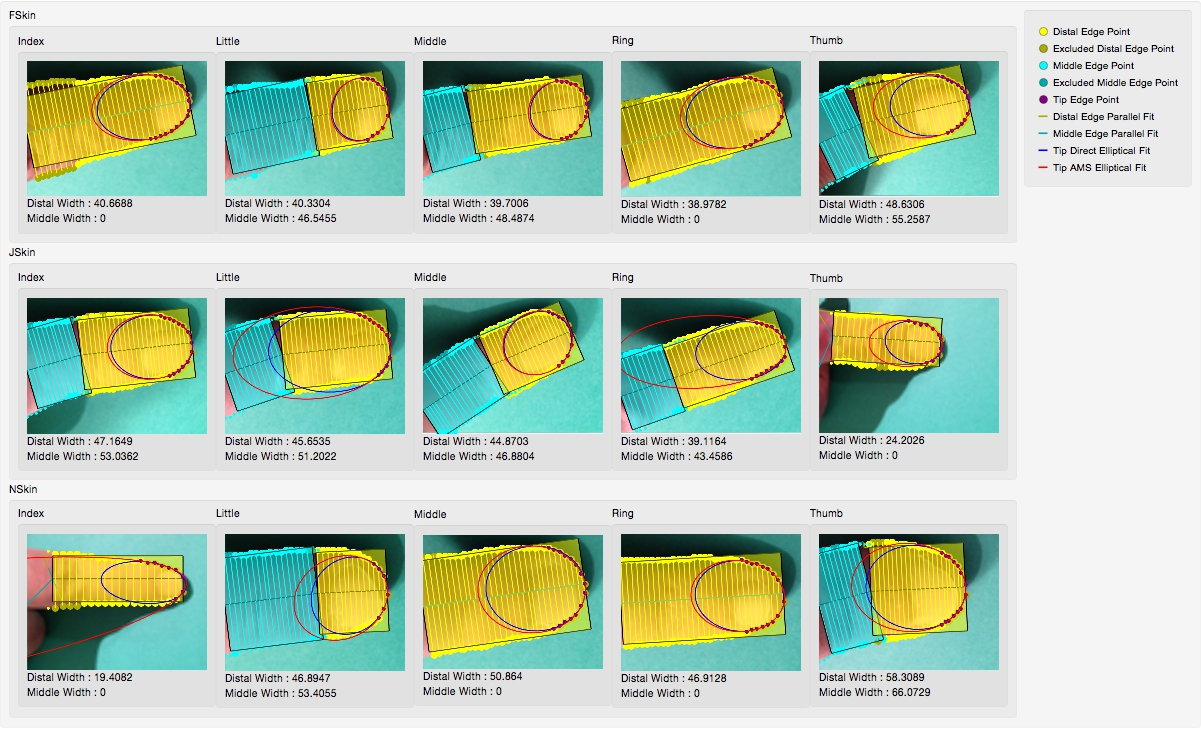
\includegraphics[width=0.95\textwidth]{Chapter4/Figs/ParallelFit.jpg}
    \caption{Initial shape-fitting stage, with the Kink Fit, midline, and Parallel Edge fit, with AMS and Direct elliptical fits to the tip.}\label{fig:ParallelFit}
\end{figure}

\subsection{Set the Scale Space}\label{sec:SetTheScaleSpace}
The images captured with the iPhone camera are large, so we define three scales: 
\begin{description}
\item[Large] The original image
\item[Medium] The image scaled relative to the width of the finger in the frame of the camera.
\item[Small] A small image just large enough to detect rapid movement between frames.
\end{description}

% We want these images to be formed without the need for re-sampling. For that reason, we restrict the choice of image sizes to those which are integer factors of the image dimensions. This is done by finding the integer factors of the original image dimensions and then selecting from those factors to scale the image. It should be noted that, to simplify point correspondences, the integer scaling from the small to medium scales is also kept.

We wish to set the mid-scale such that the number of pixels across the distal segment is over to a target value $w_m$. We are restricting the choice of scales to integer factors of the original and integer multiples of the small scale for efficient and accurate transformations of points and images. For the iPhone images the factors are:
\begin{align}
scale &= 2^{-i} 3^{-j} 17^{-k}  & i &\in \{0,1,2,3,4\} 
&  j &\in \{0, 1\} 
& k &\in \{0, 1\}
\end{align}

The small scale space is made using the largest number of small factors as possible to achieve the desired image size. This gives the greatest flexibility in scaling the mid-size.
\begin{table}[h]
\centering
\begin{tabular}{|cc|cc|c|c|c|c|c|l|}
\cline{5-10}
\multicolumn{3}{c}{ }  & & $0$ & $1$ & $2$ & $3$ & $4$ & i\\
\cline{1-10}
k & $k_{scale}$ &j & $j_{scale}$ & $1$ & $\frac{1}{2}$ & $\frac{1}{4}$ & $\frac{1}{8}$ & $\frac{1}{16}$ & $i_{scale}$\\
  \hline \hline
\multirow{4}{*}{$0$} & \multirow{4}{*}{$1$} & \multirow{2}{*}{$0$} & \multirow{2}{*}{$1$} & 
 2448 & 1224  &  612  & 306  & 153 & w \\
  &  &  & & 
  3264  & 1632  & 816  & 408  & 204  & h\\
  \cline{3-10}
 &  & \multirow{2}{*}{$1$} & \multirow{2}{*}{$\frac{1}{3}$} & 
 816  & 408  & 204  & 102  & 51  & w \\
 &  &  & & 
  1088  & 544   & 272  & 136  & 68  & h \\
\hline 
  \hline
\multirow{4}{*}{1} & \multirow{4}{*}{ $\frac{1}{17}$ } & \multirow{2}{*}{$0$} & \multirow{2}{*}{$1$} & 
 144  & 72  & 36  & 18  & 9 & w \\
 &  & & & 
  192  & 96  & 48  & 24  & 12  & h \\
    \cline{3-10}
 &  &  \multirow{2}{*}{$1$} & \multirow{2}{*}{$\frac{1}{3}$} & 
 48  & 24   & 12  & 6   & 3 & w \\
   &  &   & & 
  64  & 32  & 16  & 8  & 4  & h \\
\hline 
\end{tabular}
\caption{The image pixel dimensions for all possible integer factor scalings.}
\end{table}

So for a chosen small scale $S_s = 2^{-3} 3^{-1}$, a distal width in the small scale $w$ and a minimum distal width in the medium scale $w_m$. 
Finding  $i_m$ and $j_m$ which minimise $i_m + \frac{\log(3)}{\log(2)} j_m$  and which satisfy  $2^{-i_m} 3^{-j_m} - \lceil \frac{w_m}{w} \rceil \ge 0$, $i_m\le i_s$ and $j_m \le j_s$ determines the medium scale space.

\subsection{Modelling the Fingertip}\label{sec:ModellingTheFingertip}
\begin{figure}[p!]
  \centering
  \noindent
  
  \begin{tabular}{cc}
  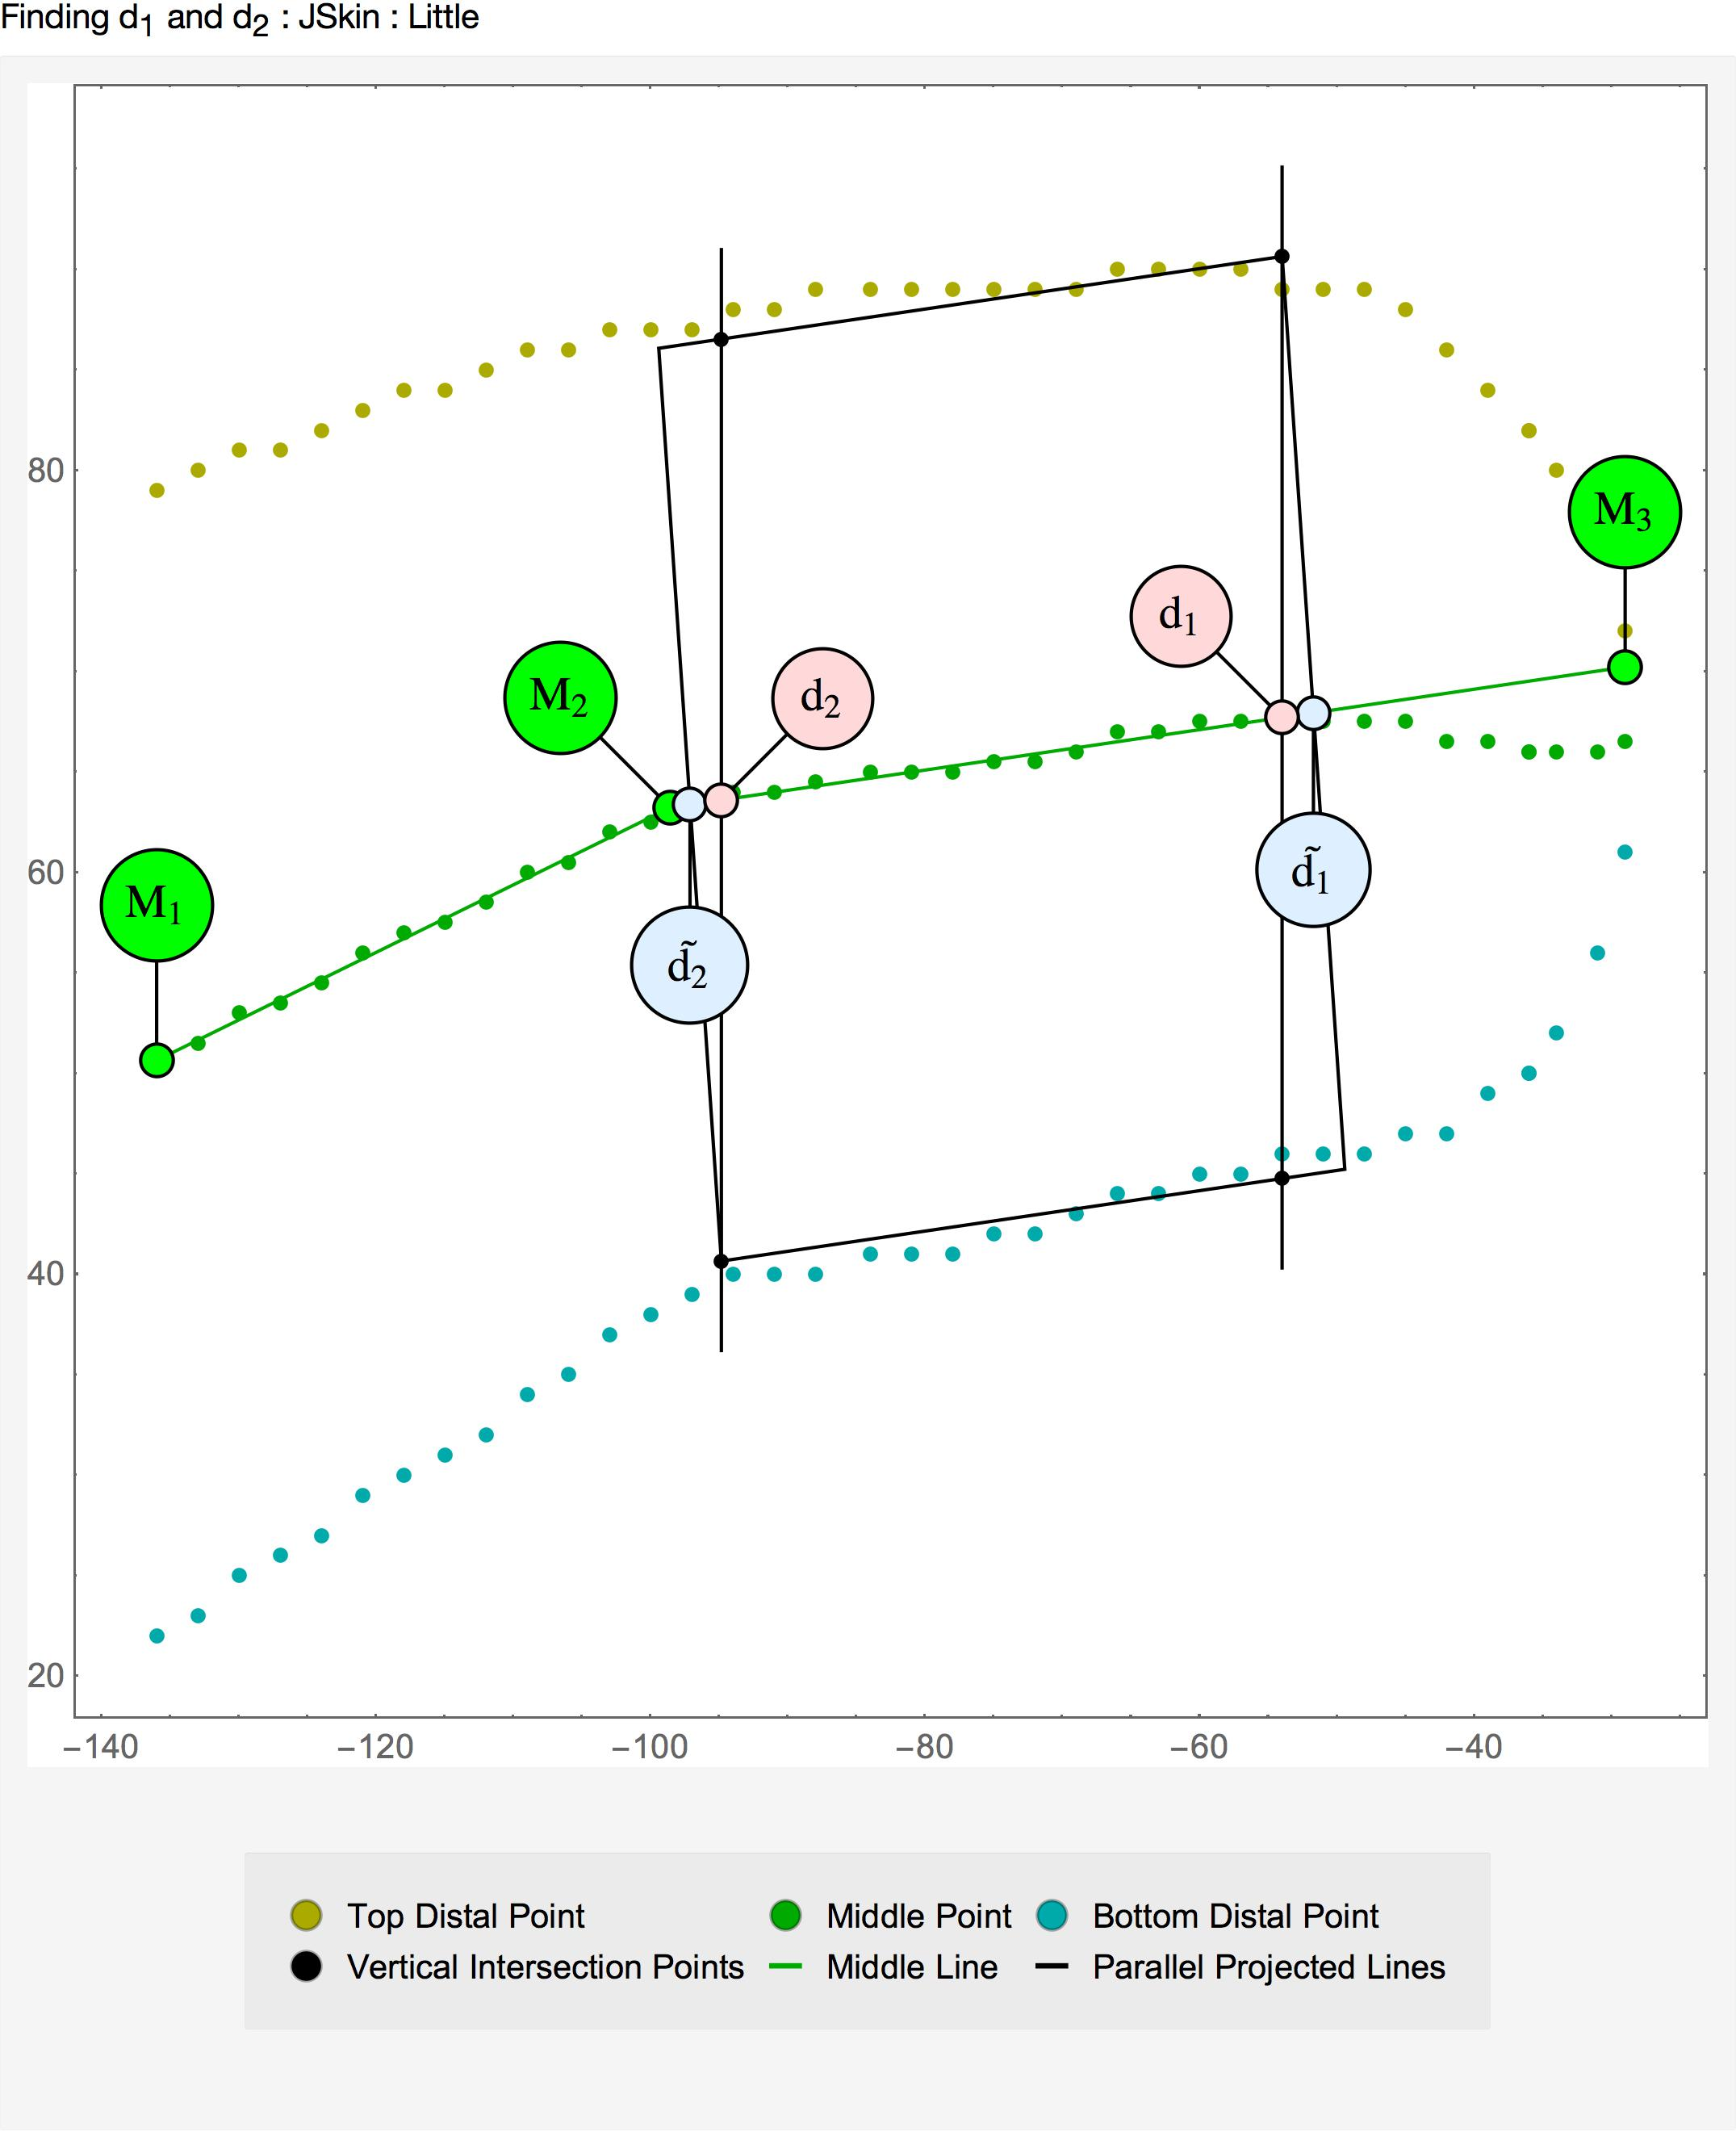
\includegraphics[width=0.45\textwidth, height=0.5\textwidth]{Chapter4/Figs/Model_FindingD1AndD2_JSkin_Little.jpg} &
    \parbox[b][0.5\textwidth][s]{0.55\textwidth}{
   \textbf{a) Determining $d_1$ \& $d_2$} --- We have a midline which is given as two points $M_2$ \& $M_3$; one somewhere on the digit ($M_2$), and the other at the tip ($M_3$). If the finger were straight in the frame, then $d_1=\tilde{d_1}$ and $d_2=\tilde{d_2}$ could easily be found by finding the points on that line. However, the fact that the digit can be presented at an angle means that the edge points vertically above and below the point on the midline may include part of the curved tip. This has the effect of making these midpoints diverge from the midline of the digit. This can be corrected by adjusting with half the gradient of the midline $\delta\:mid$ to the ratios. \begin{equation*}distance \:on \:line = (\frac{1}{2} + \left\lvert\frac{1}{2}\delta\:mid\right\lvert) w\end{equation*} \vfill
    } \\ 
    \parbox[b][0.5\textwidth][s]{0.45\textwidth}{
             \textbf{b) A New Midline Fit} --- We take the set of midline points, extract the subset which lies between $d_1$ and $d_2$, and then apply a straight line fit to these points. The origin is the fit evaluated at the $x$ component of $d_2$, and we determine an orientation $\theta$, which is $\arctan$ the gradient of the linear model. \vfill
        } &
        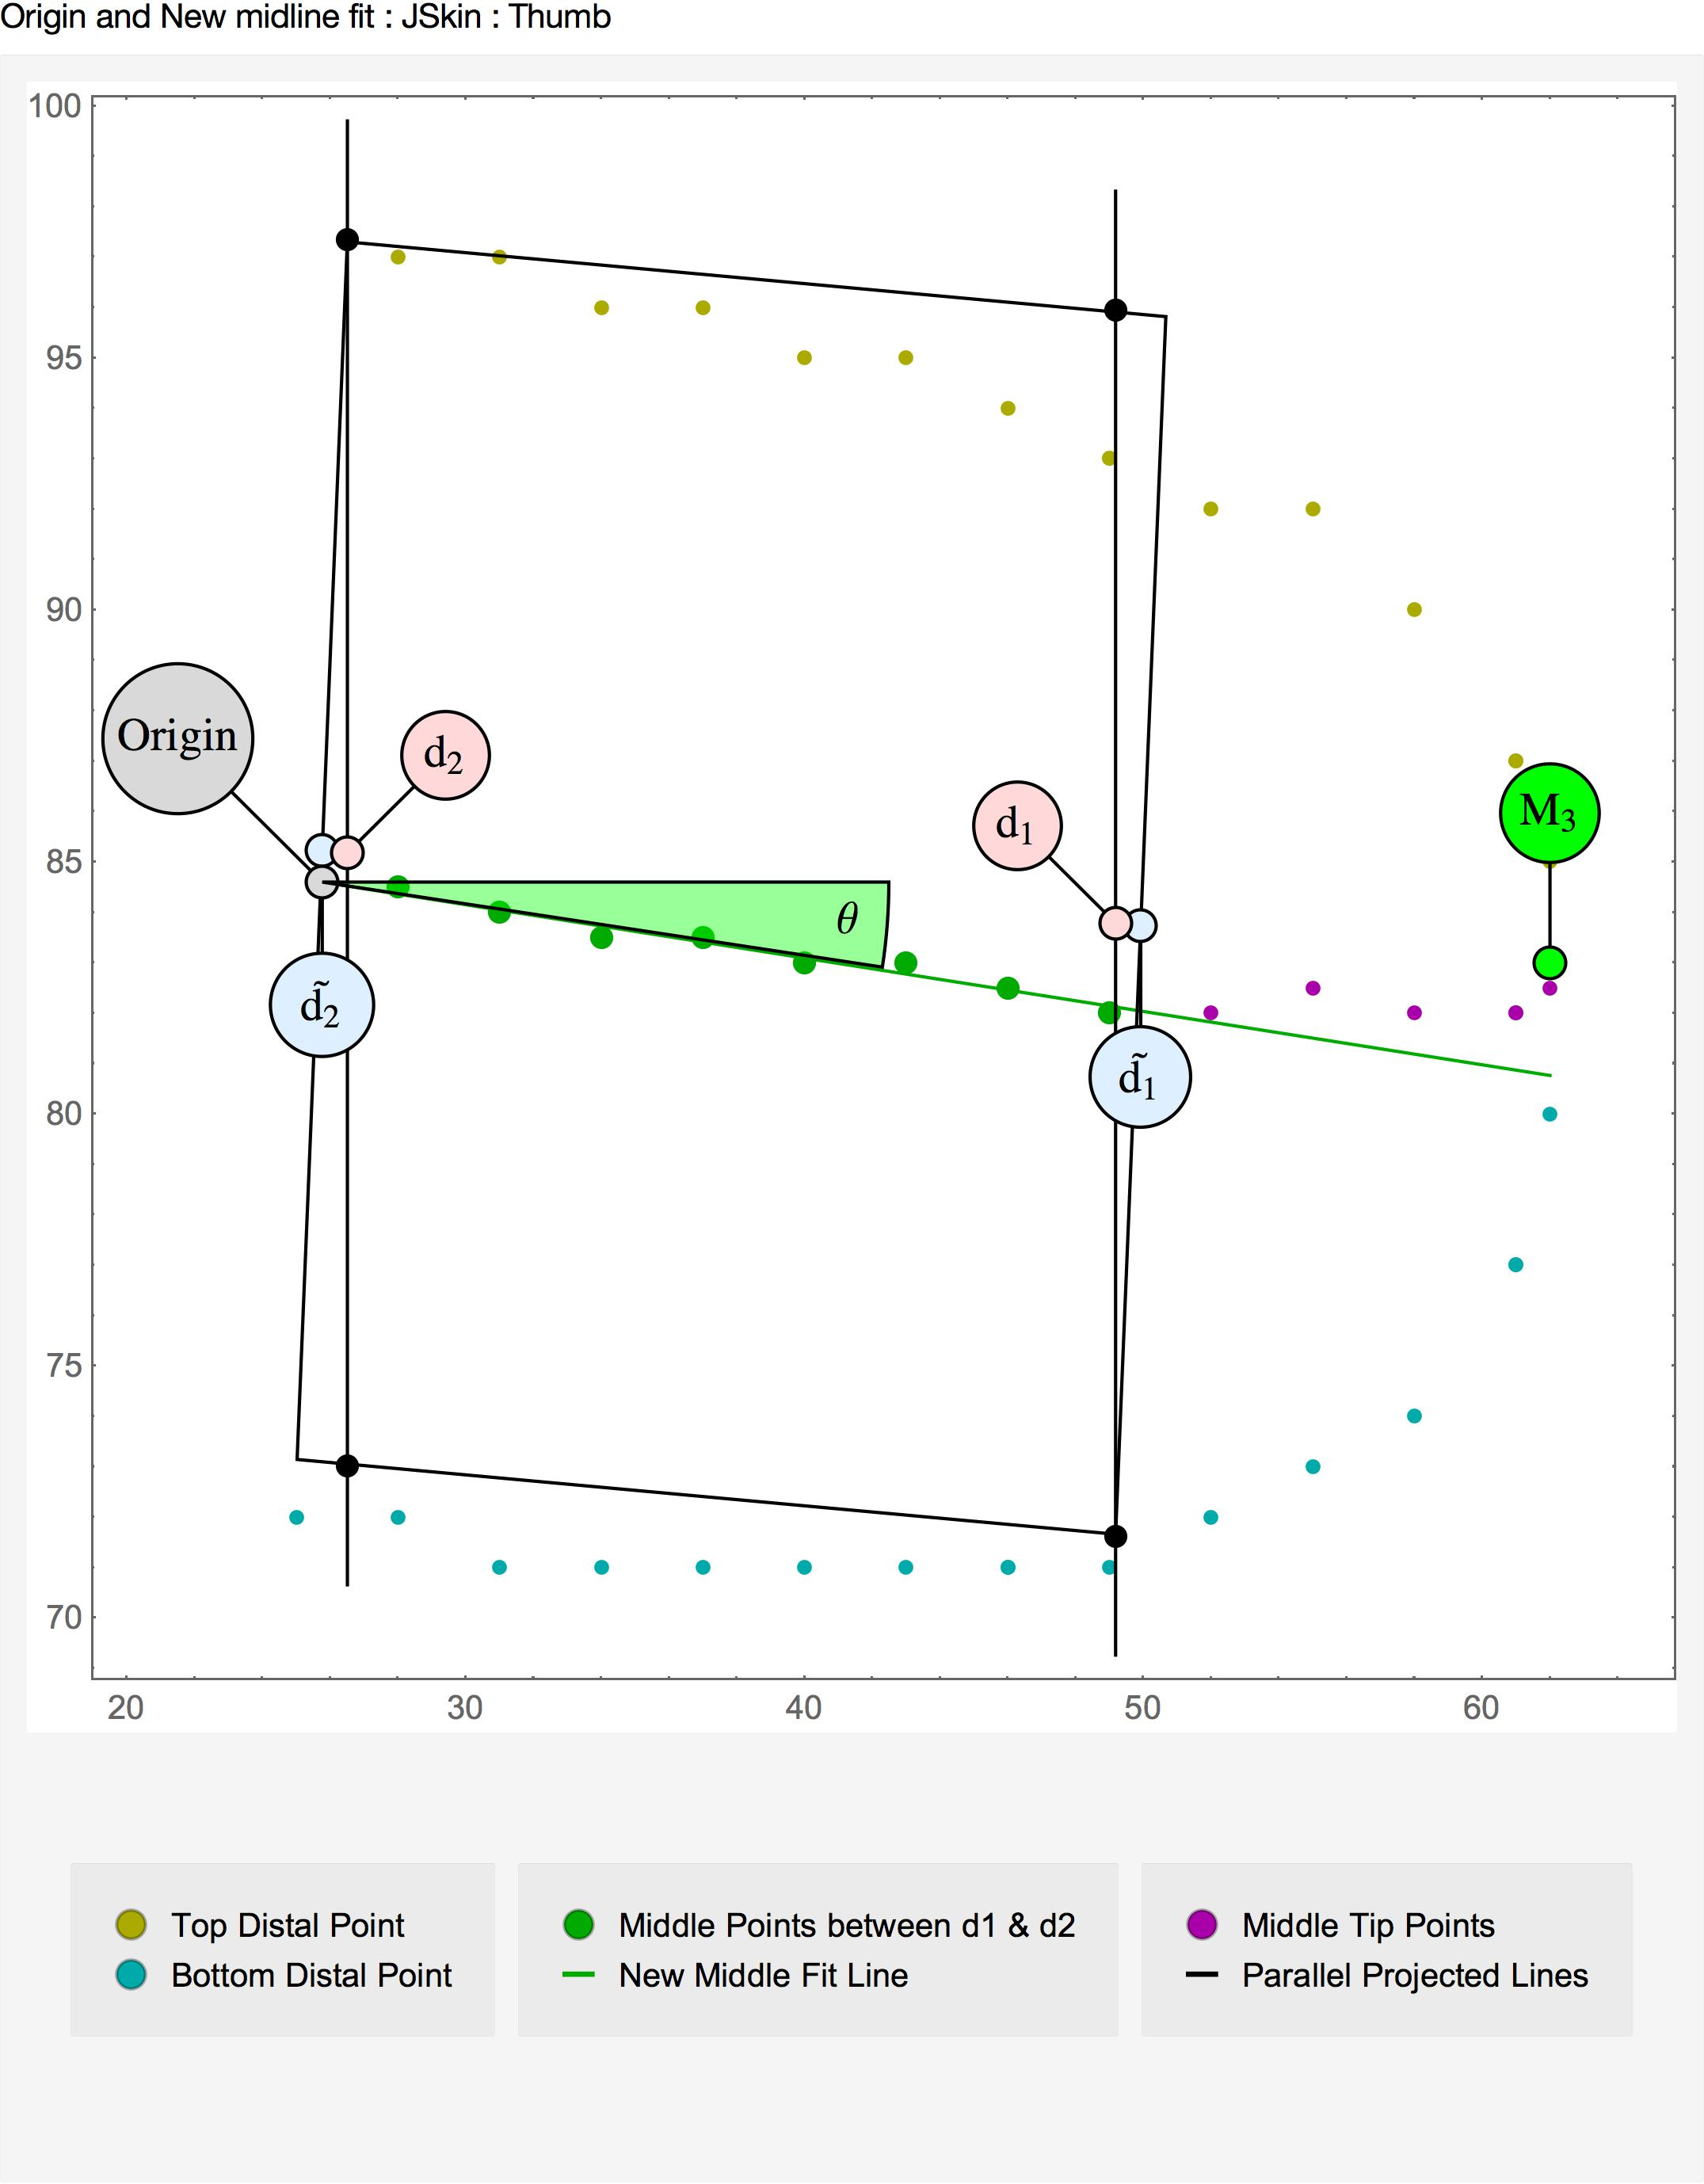
\includegraphics[width=0.55\textwidth, height=0.5\textwidth]{Chapter4/Figs/Model_Midline_JSkin_Thumb.jpg} 
    \\ 
   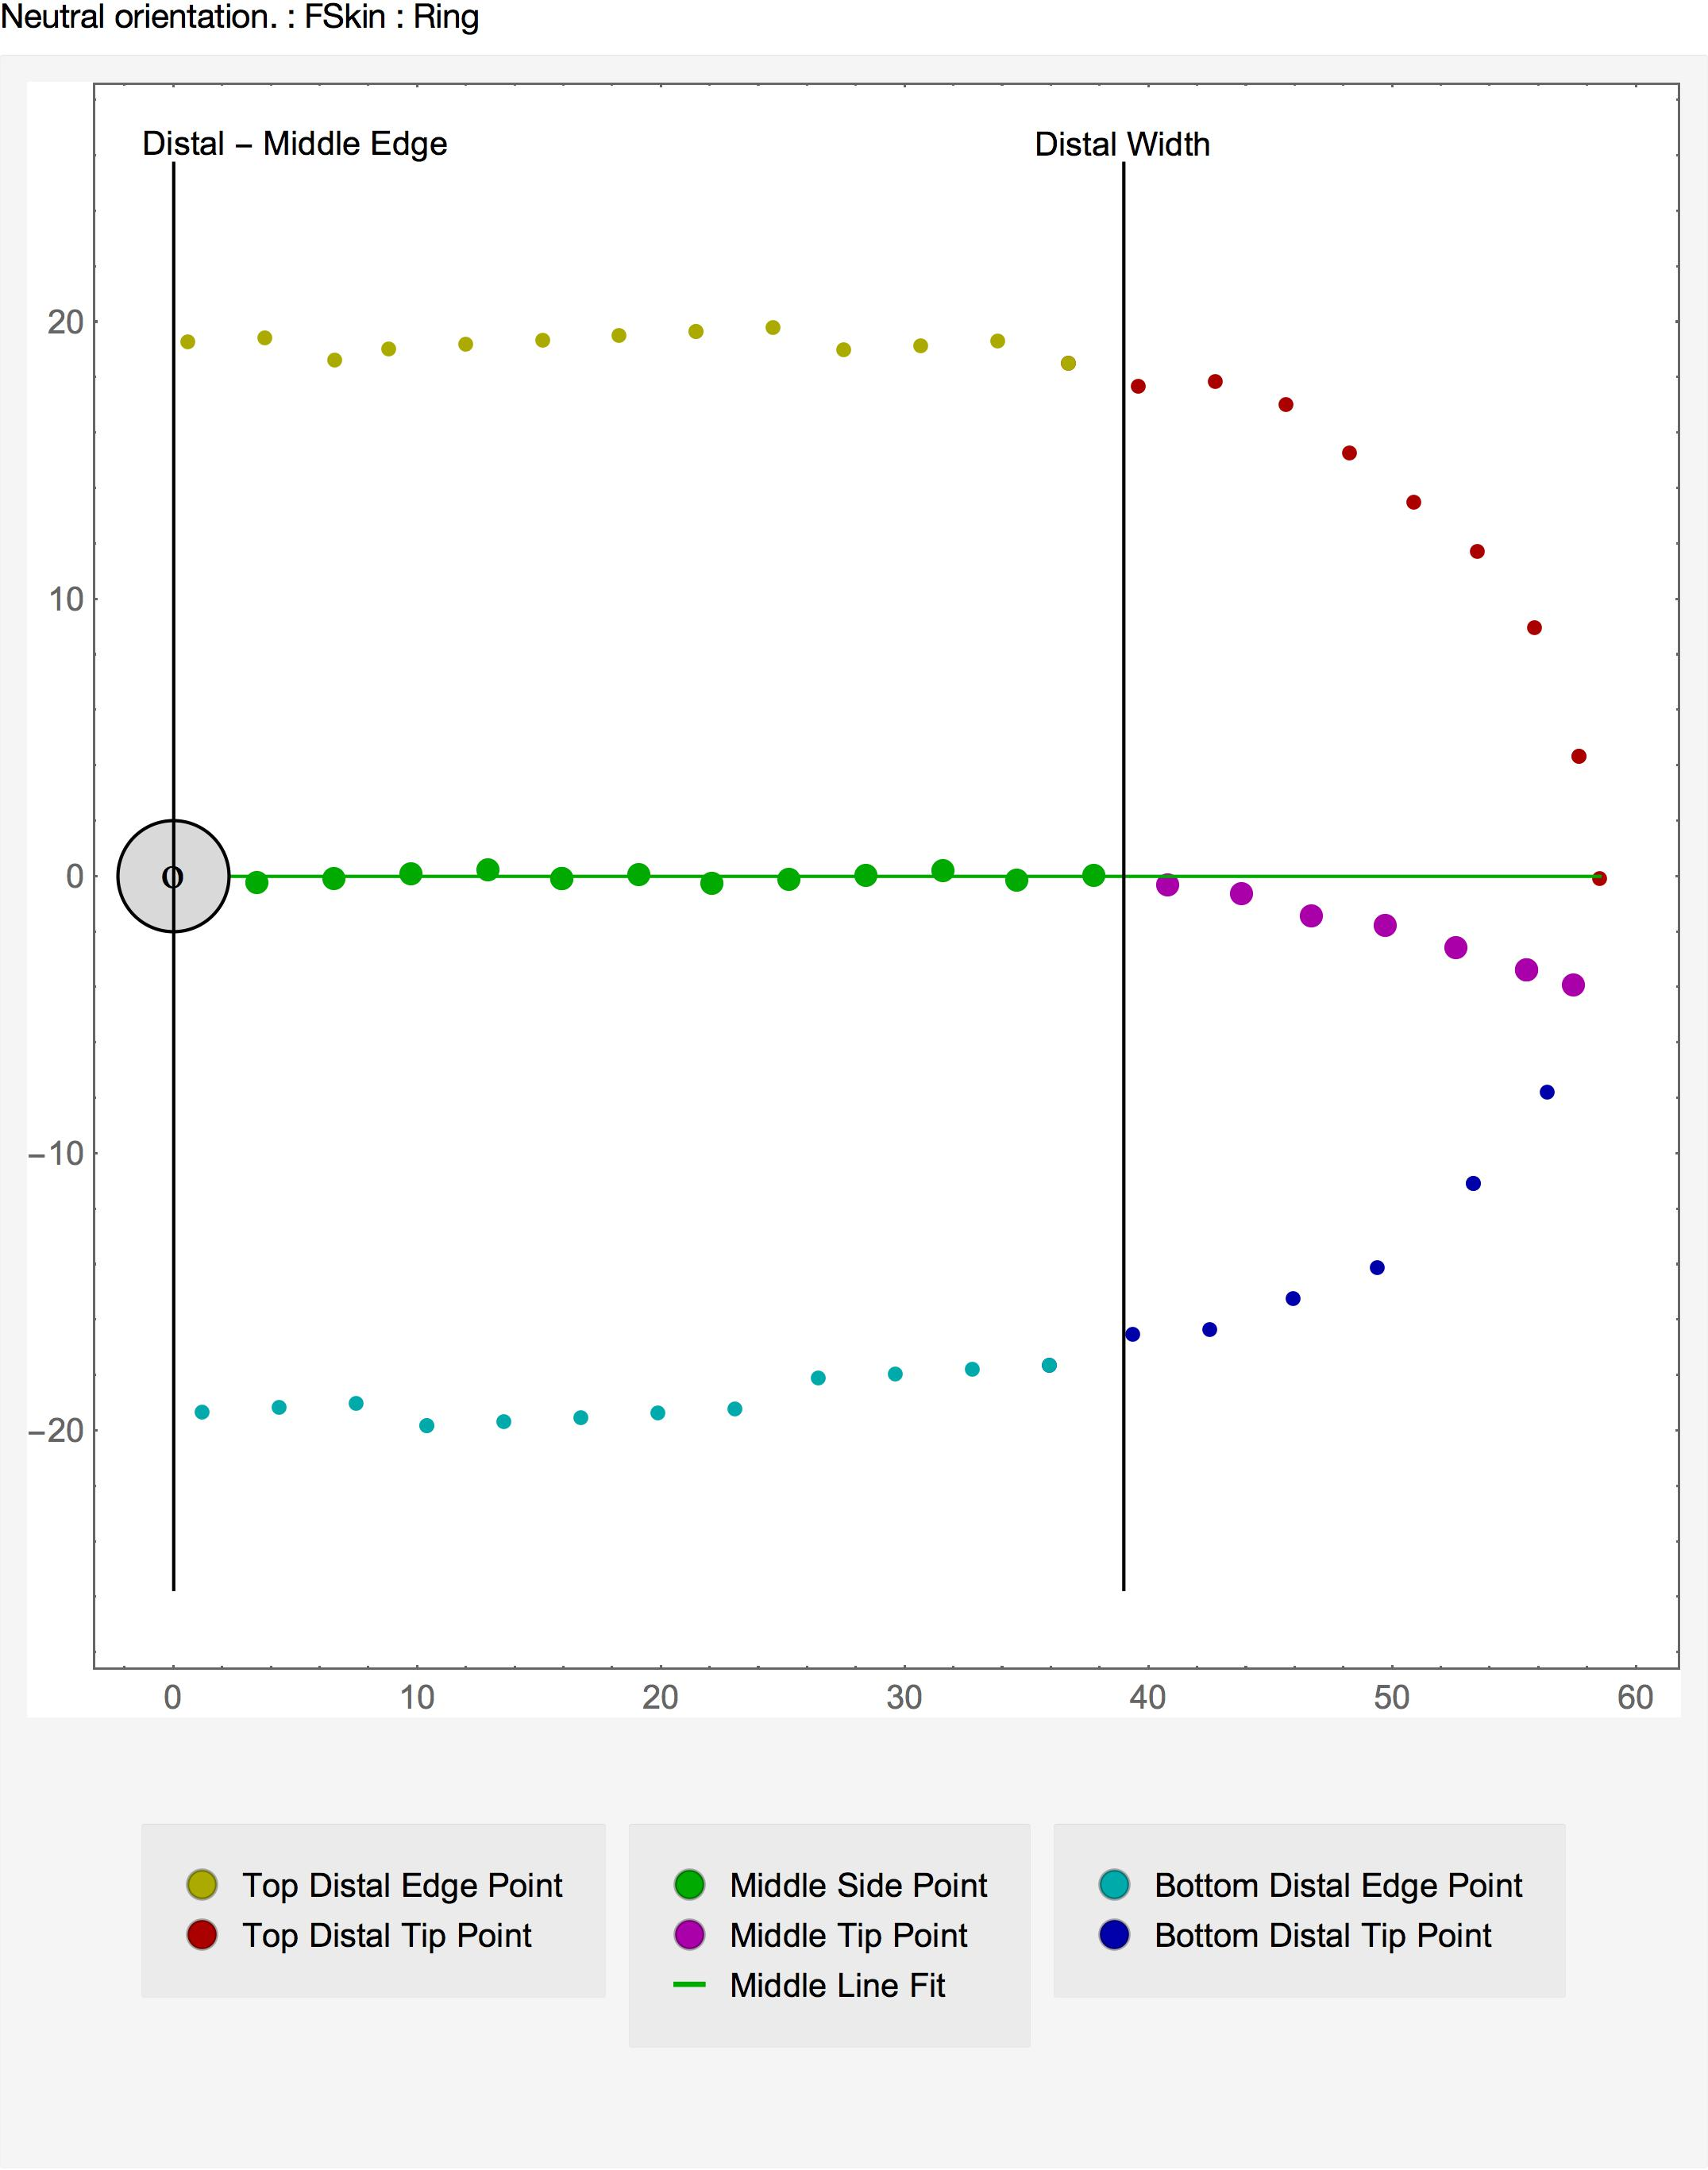
\includegraphics[width=0.45\textwidth, height=0.5\textwidth]{Chapter4/Figs/Model_NeutralCoords_FSkin_Ring.jpg} &
    \parbox[b][0.5\textwidth][s]{0.55\textwidth}{
         \textbf{c) Determine the Neutral Coordinates} --- We move all the points --- the top and bottom edges, and the midline points --- and we translate to the new origin. Then, we rotate by $-\theta$. This we call the "neutral coordinates", as the tip is aligned with its midaxis lying on the $x$ axis. These points are separated at one distal width from the tip; a Trapezian fit is applied to one set of points, and an Elliptical fit is applied to the other. As a refinement to this, although the linear fit is applied as in the Trapezian section, the algorithm then looks at the points beyond and before the one distal width region; if they're consistent with the fit, then they are considered still part of the straight edge. The Elliptical fit is applied as discussed previously. \vfill
    }
    \end{tabular}\\
    \phantomcaption
\end{figure}
\addtocounter{figure}{-1}

\begin{figure}[p!]
\ContinuedFloat
\centering
\begin{minipage}[t]{1\textwidth}
\begin{wrapfigure}{l}{0.5\textwidth}
  \begin{center}
    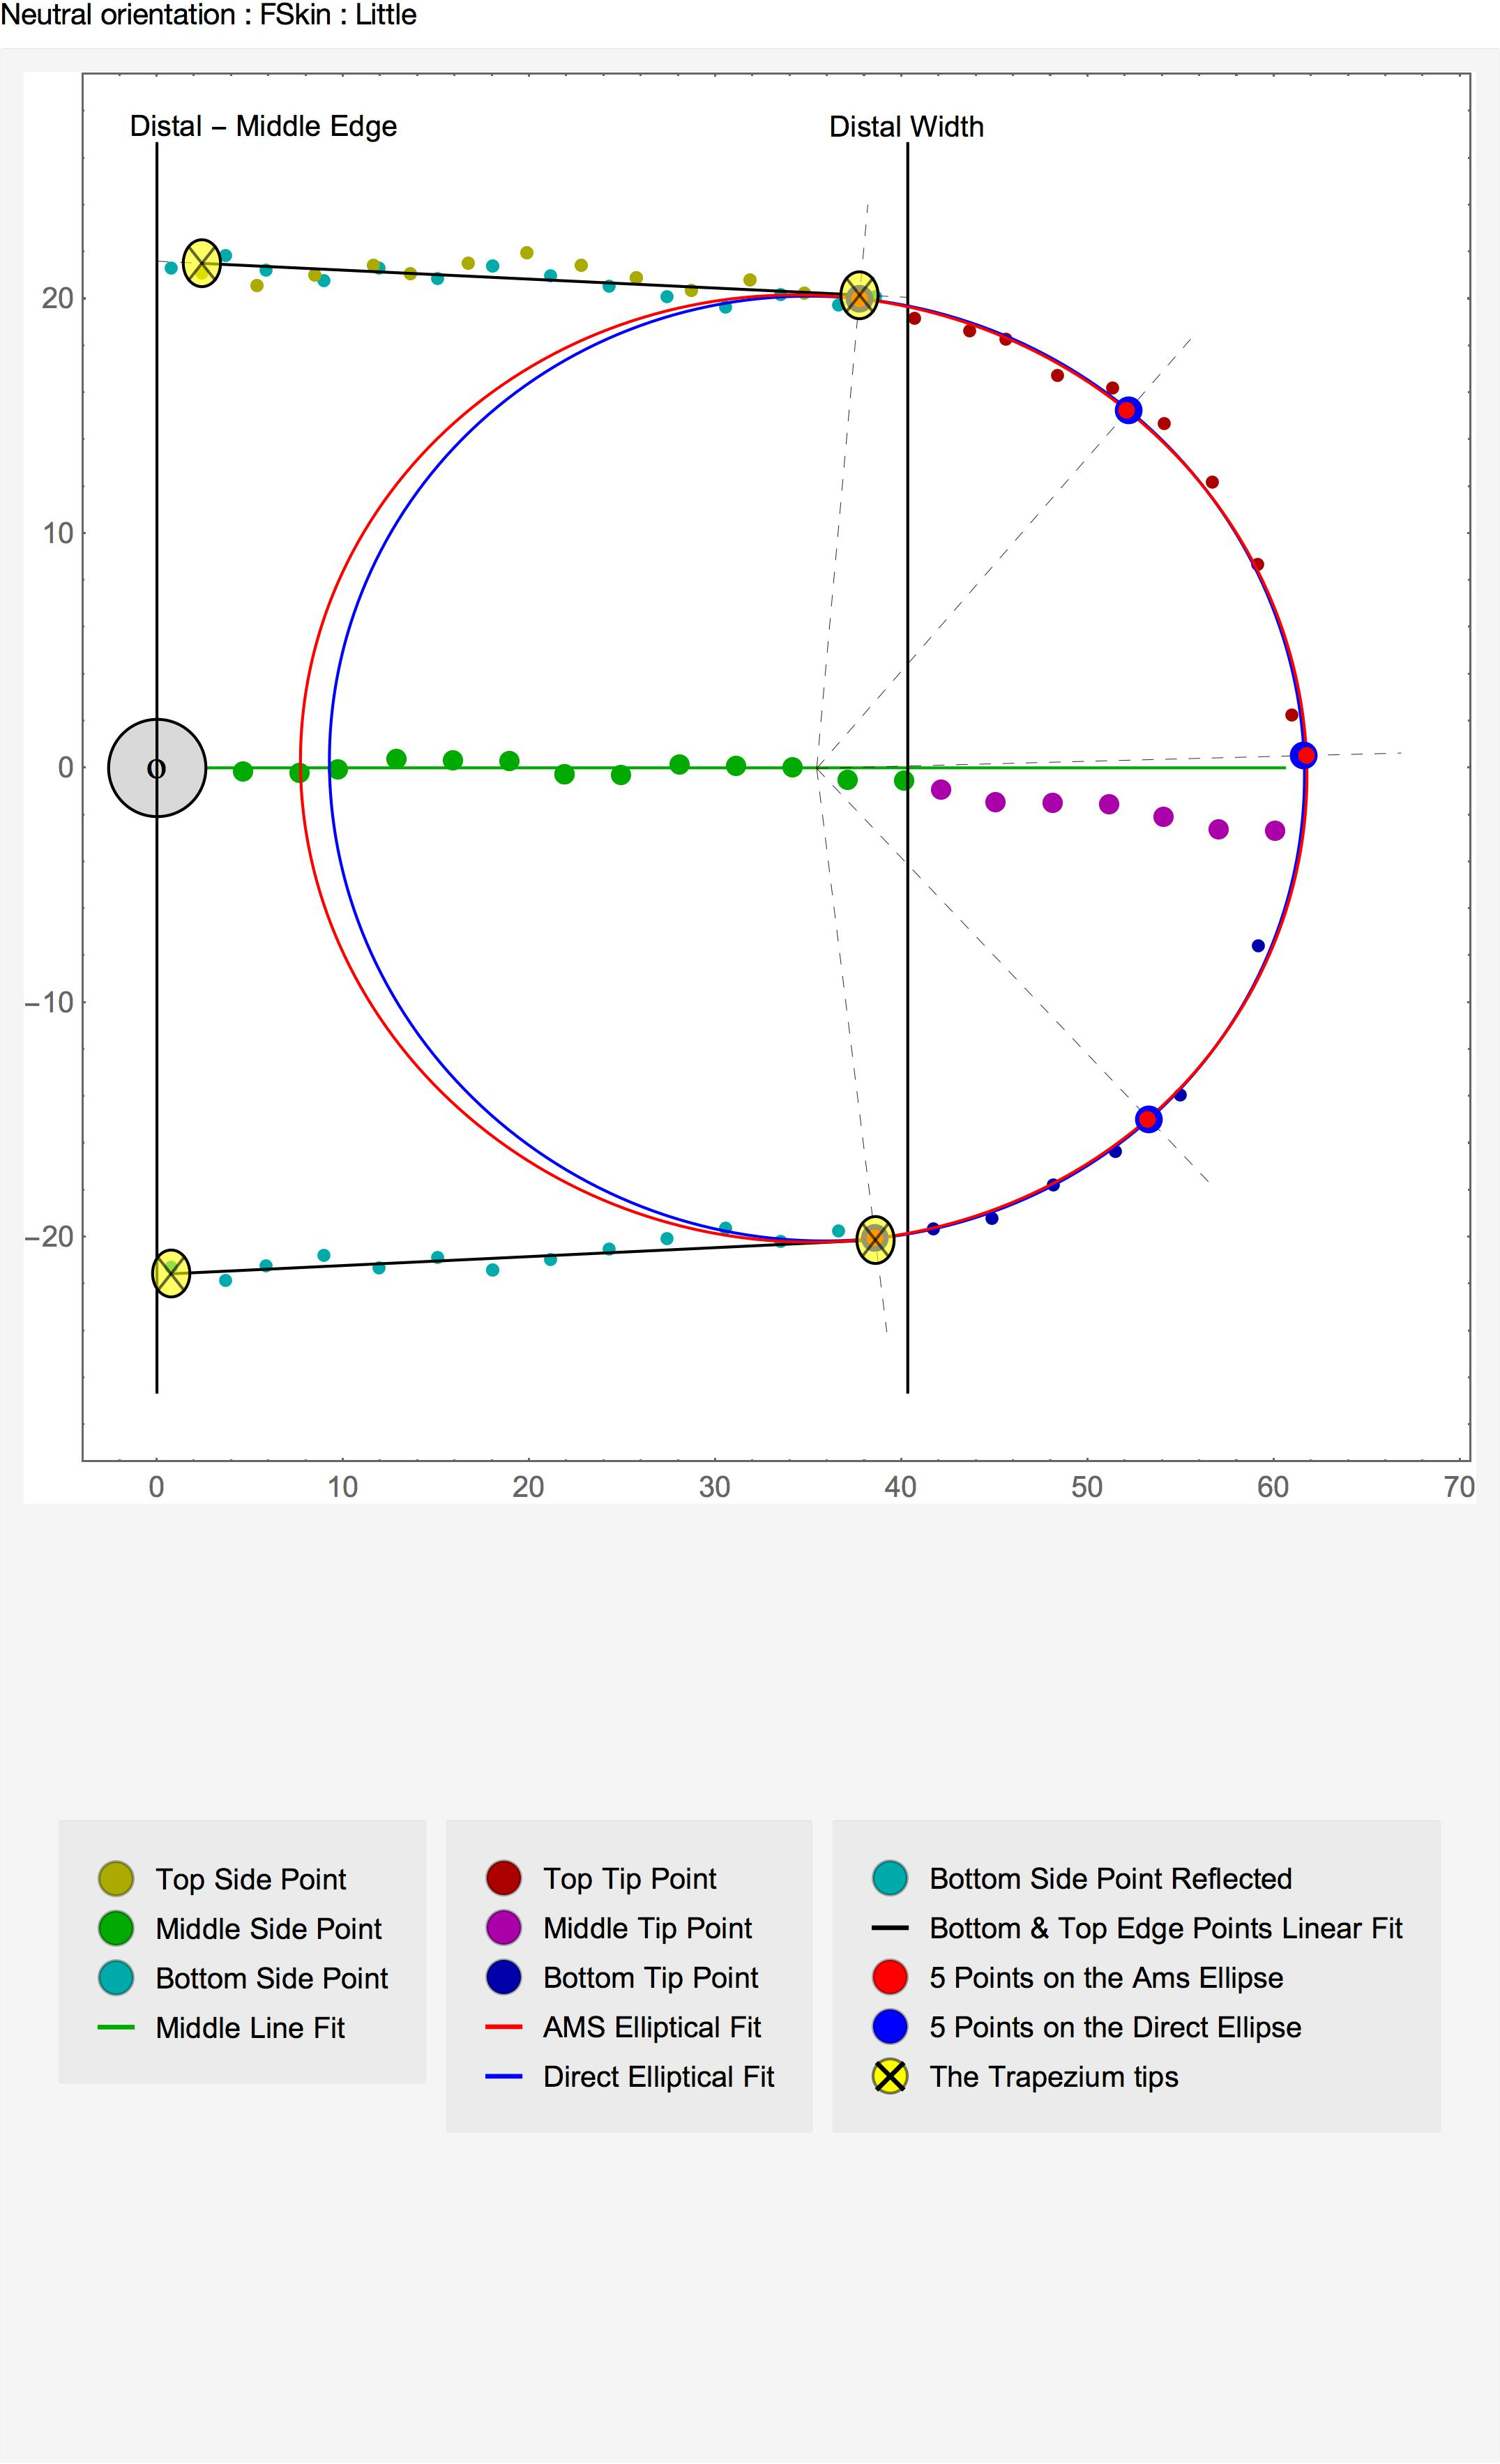
\includegraphics[width=0.5\textwidth]{Chapter4/Figs/Model_ShapeFitting_FSkin_Little.jpg}
  \end{center}
  \phantomcaption
\end{wrapfigure}
         \textbf{d) Fitting the Shapes} --- The comparison between the elliptical fit methods is done by looking at the distance from the front two points on the trapezium to the edge of the ellipse, and the best of these is chosen. Unfortunately, this is often not sufficient to make the ellipse join with the trapezium exactly because further on in the algorithm, these shapes will be used to perform a mask; we want to avoid introducing artefacts which could be interpreted as features. So, we wish to remove these discontinuous intersections between the ellipse and the trapezium. In order to do this, we choose three points on the Elliptical fit and the two front points of the trapezium, thereby making a set of five points, and we pass these through the direct Elliptical fit algorithm. It should be noted that five points is what is required to completely define an ellipse; there is only one ellipse which will pass through five points.
    \end{minipage}
    \subfloat{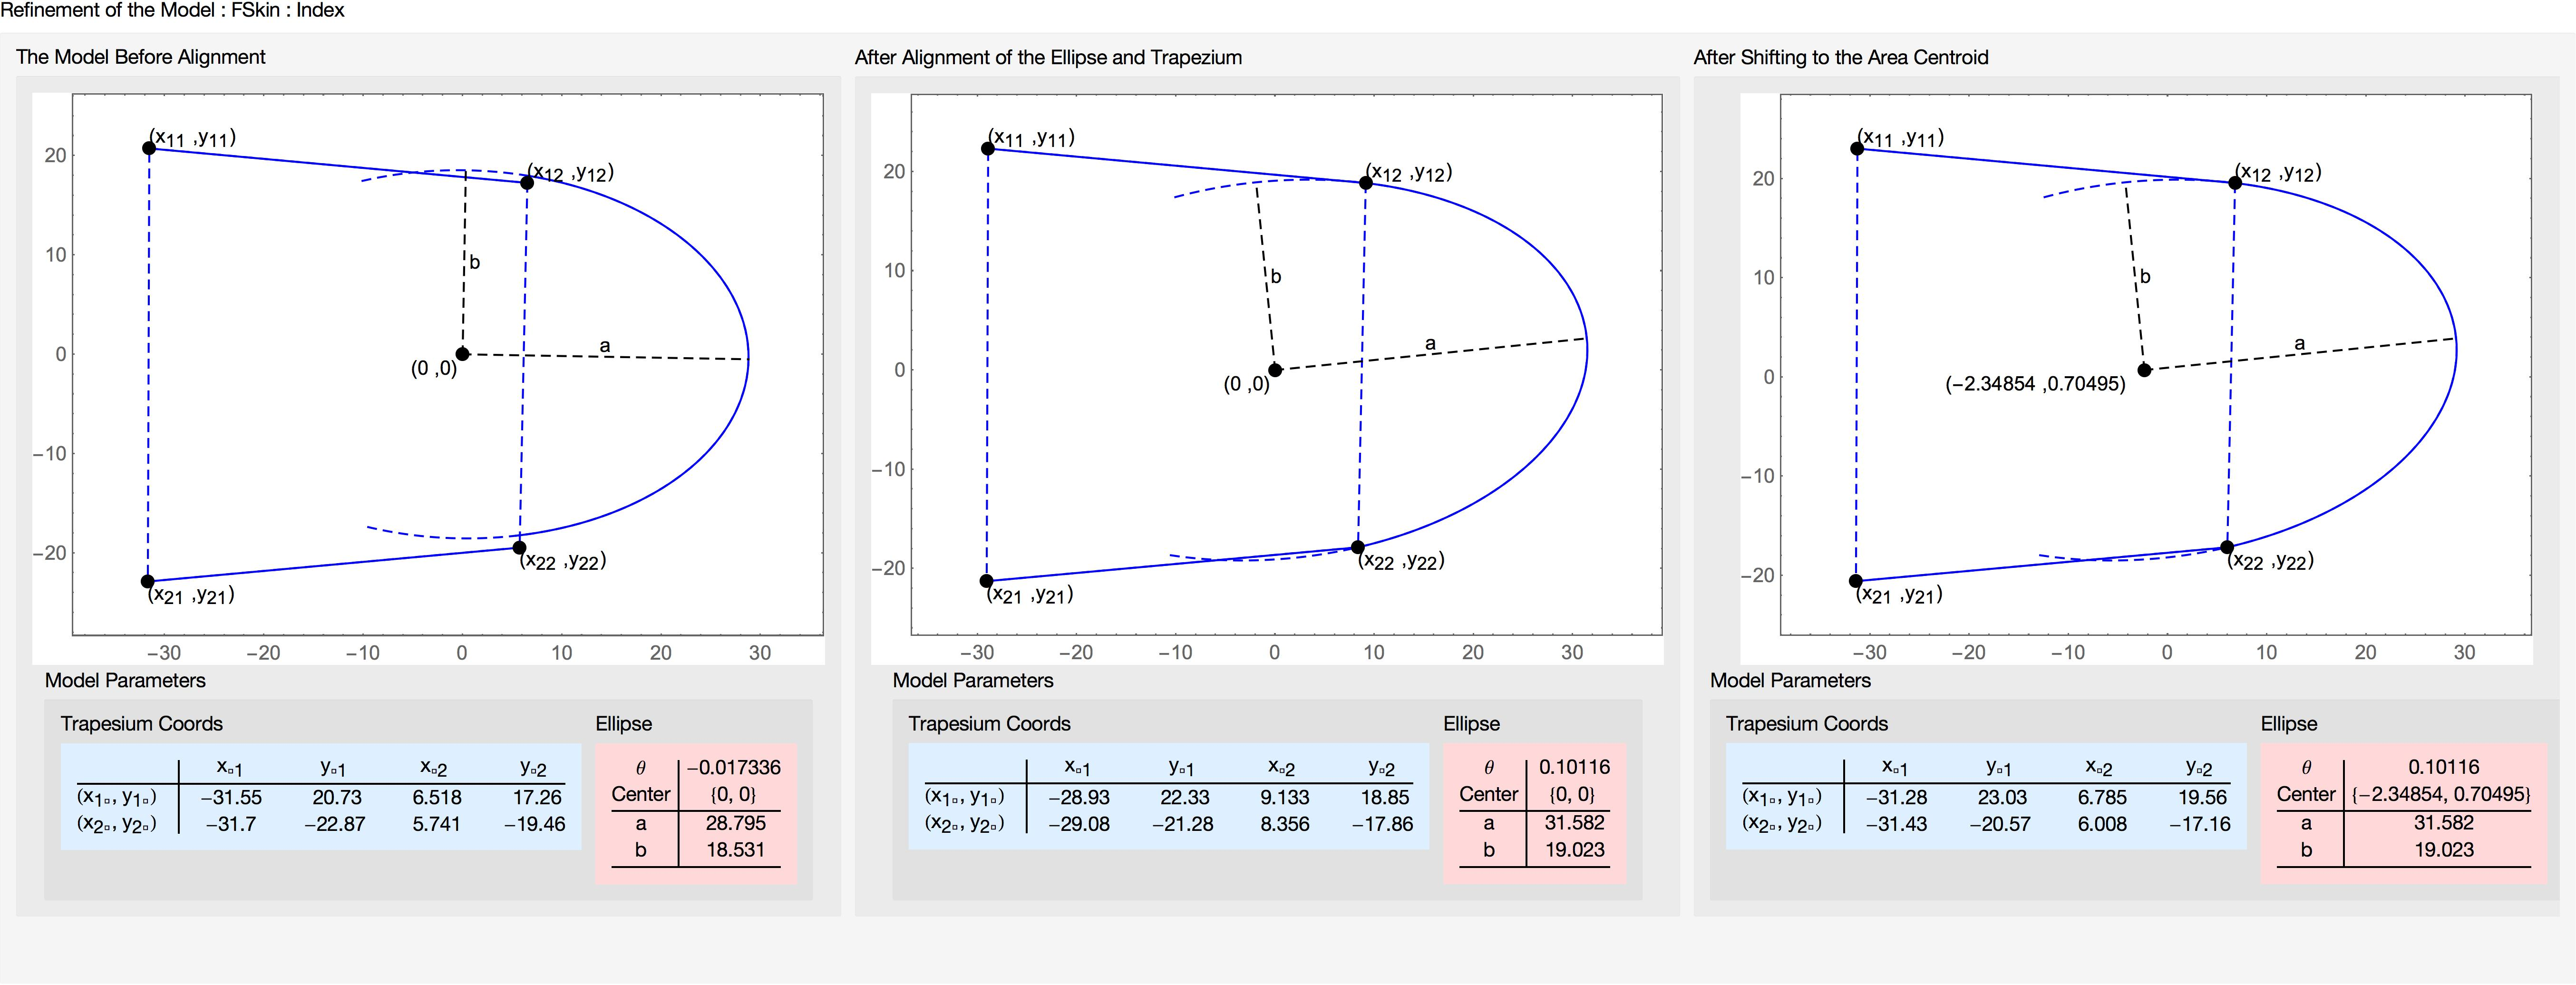
\includegraphics[width=0.99\textwidth]{Chapter4/Figs/Model_Finalizing_FSkin_Index.jpg}}\\
    \begin{minipage}{0.95\textwidth}
         \textbf{e) Finalizing the Model} --- The coordinates for the ellipse and the trapezian are adjusted so that the origin is at the center of the ellipse, and the ellipse has zero rotation. The reason for this is that it makes calculating the distance from the edges of the ellipse easier. So, now when we apply the model to the image, all that's required is a position --- which is the position of the center of the ellipse --- and an orientation about that position. 
    \end{minipage}
    \caption{The Fingertip Model Algorithm.}\label{fig:ModelingFingertip}
\end{figure}

Having determined a measure of the width of the distal portion of the fingertip allows for a more robust model of the fingertip to be determined. This is because the measurement of the distal width is far more reliable than the distal length which has so far been determined, as the distal length has been found by evaluating where the "kink" of the midline points lies. For example, if the distal joint is un-flexed, the knuckle portion will be overlooked entirely, as seen in Figure \ref{fig:ParallelFit}. It turns out that the average anatomical ratios of the distal,  middle, and  proximal lengths $2:3:5$ and the width $w$ to distal length $l_{d}$ ratio $2 : 3$  is a far more reliable method of determining the distal length $l_{d} = 1.5 w$.

From the kink fit, we have a midline, which is specified by three points. We now determine two points on this line, which are $\frac{1}{2}$ the distal width ($d_1$) and $1\frac{1}{2}$ the distal width from the tip ($d_2$). So the midline point that lies between the two points can now be taken to correspond to the straight-edged section of the distal portion of the finger. These points are passed to the Trapezian Fit method (\ref{sec:TrapezianFit}), and the points which lie between the tip and the point half the distal width from the tip are passed to the Elliptical Fit (\ref{sec:EllipticalFitMethod}). The ellipse is adjusted to correspond with the two near vertices of the Trapezian; the result can be seen in Figure \ref{fig:ModelingFingertip}.

\begin{figure}[h!]
  \centering
    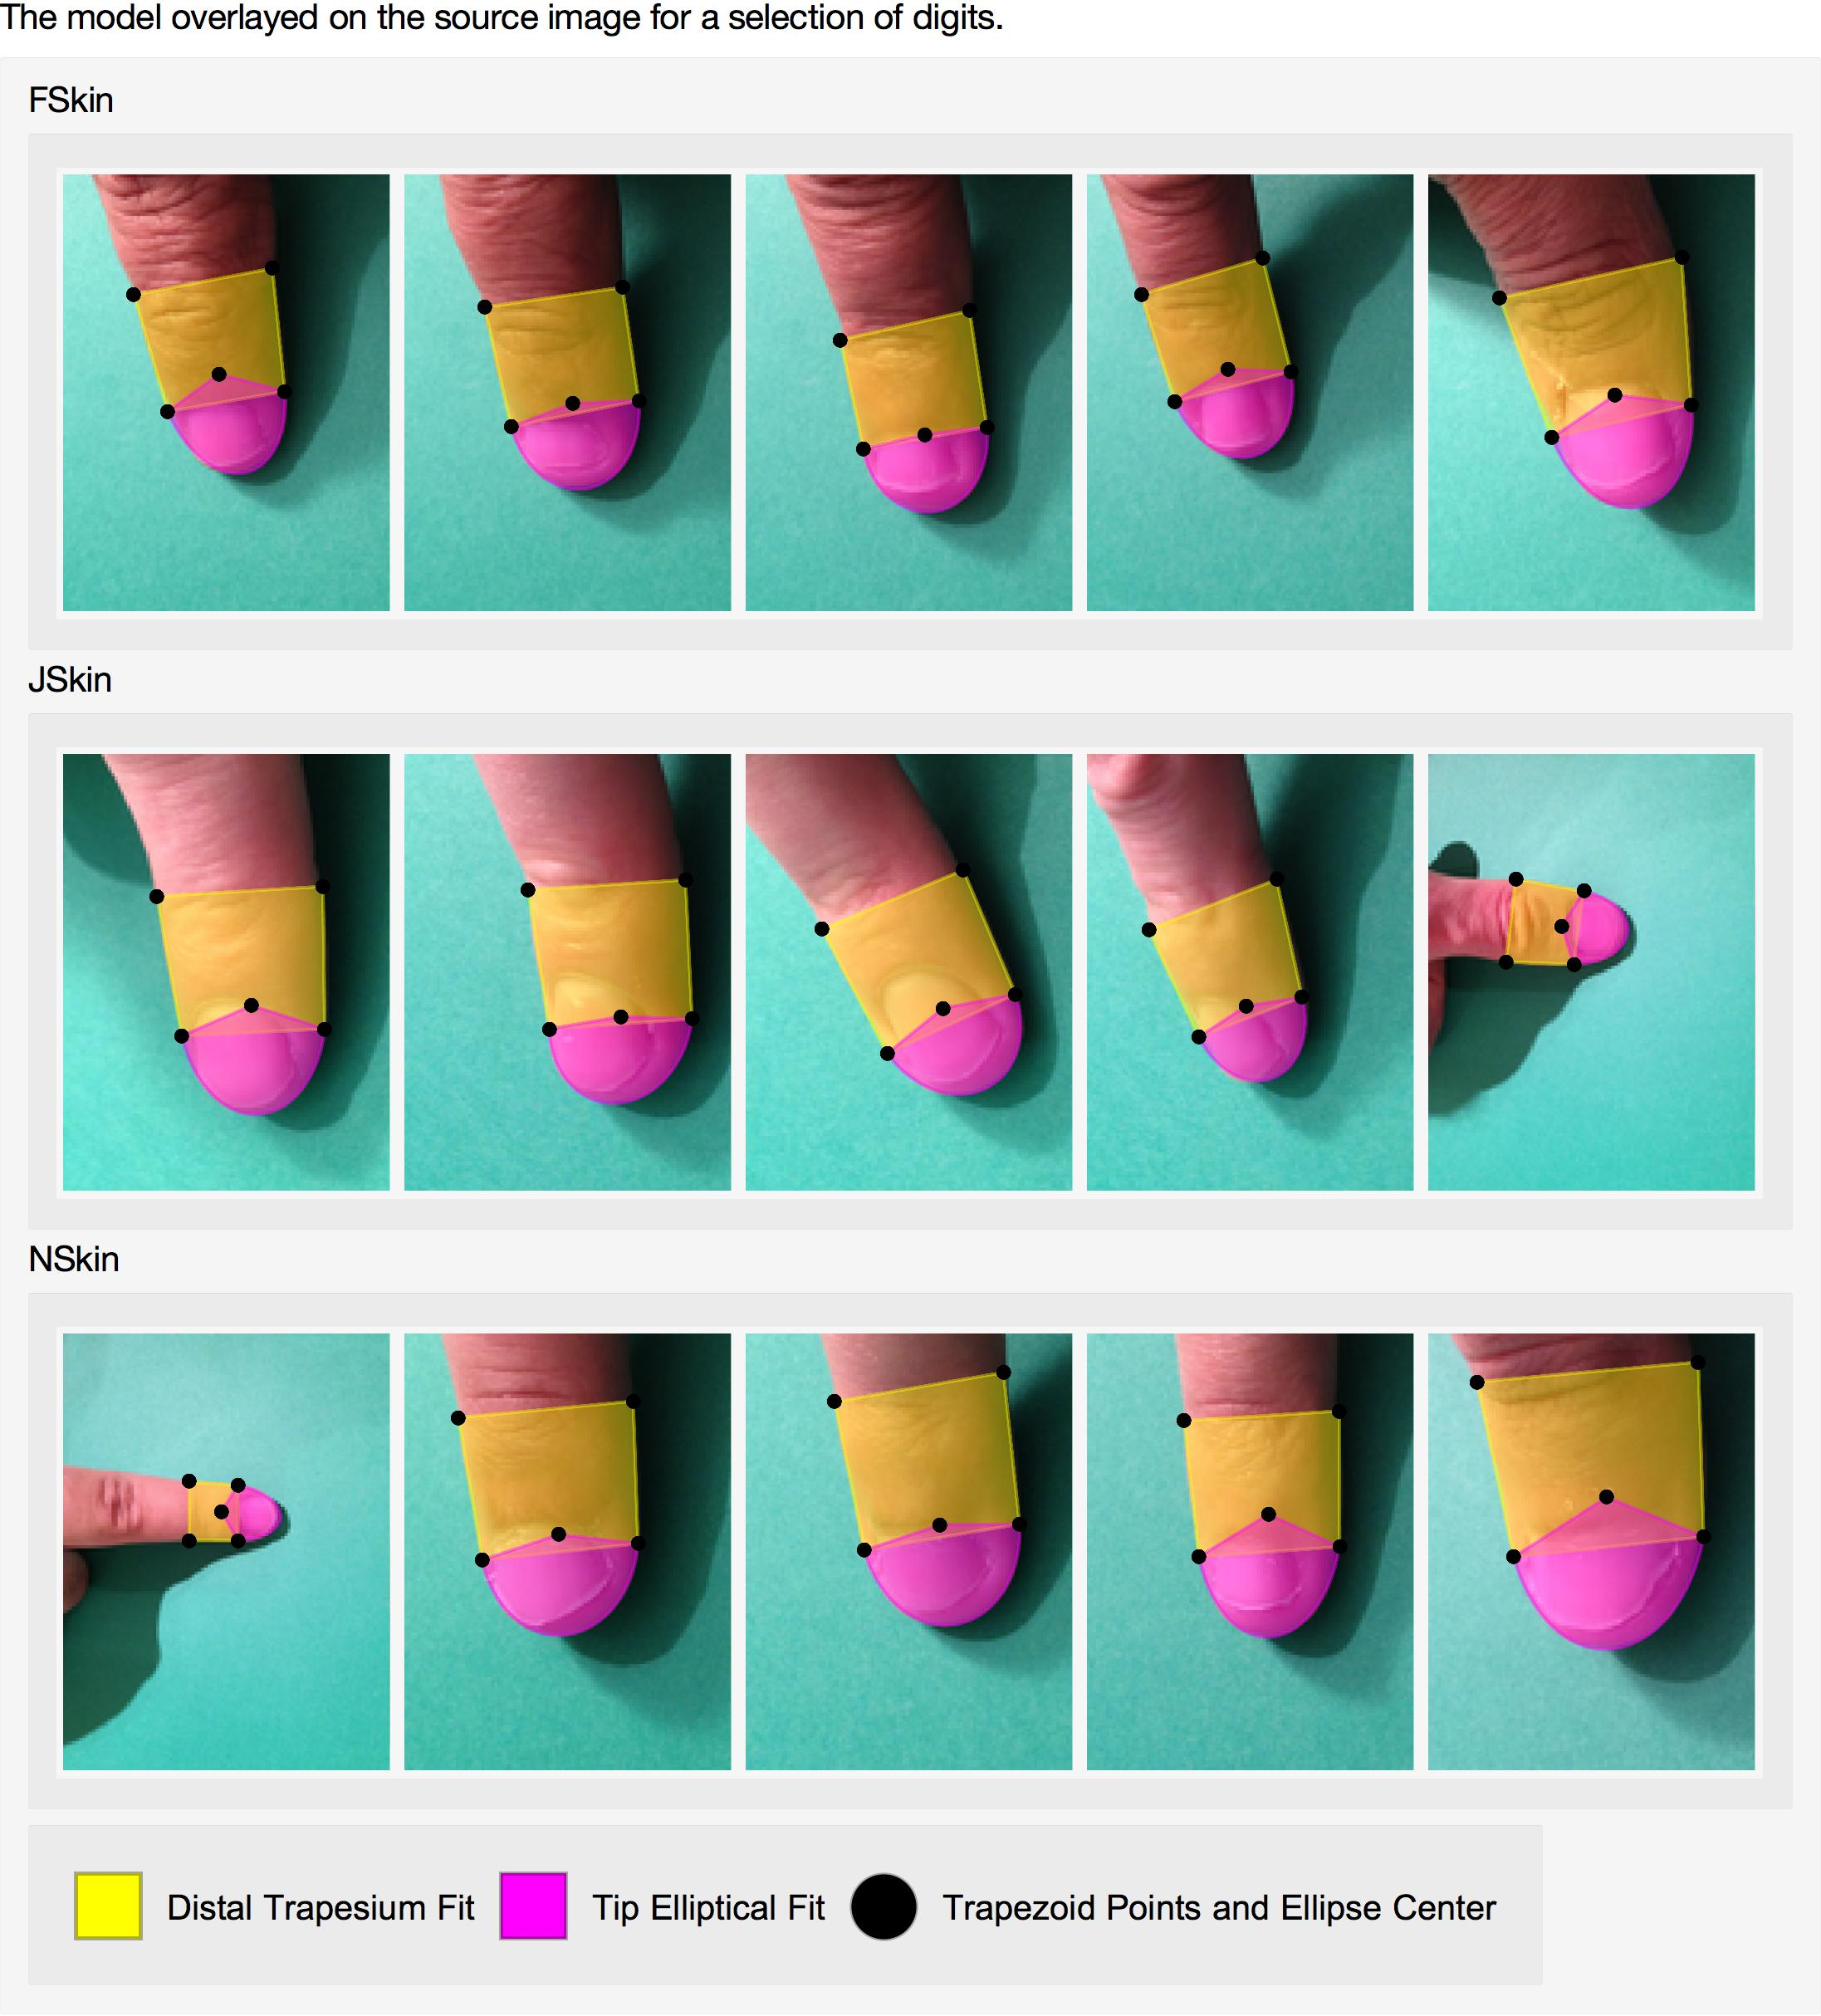
\includegraphics[width=0.99\textwidth]{Chapter4/Figs/Model_Overlayed.jpg}
    \caption{The models overlayed on the source images.}\label{fig:FingertipModelResult}
\end{figure}

Overlaying the model on its source image shows that the application of the model actually only requires a position and orientation, because we assume that the camera is positioned such that the digit presents at the same scale when in contact with a surface throughout the frame; we're not accounting for perspective effects in this simple application.
The model can be seen overlayed on the selection of digits for three individuals in Figure \ref{fig:FingertipModelResult}.


\begin{sidewaysfigure}[h!]
  \centering
    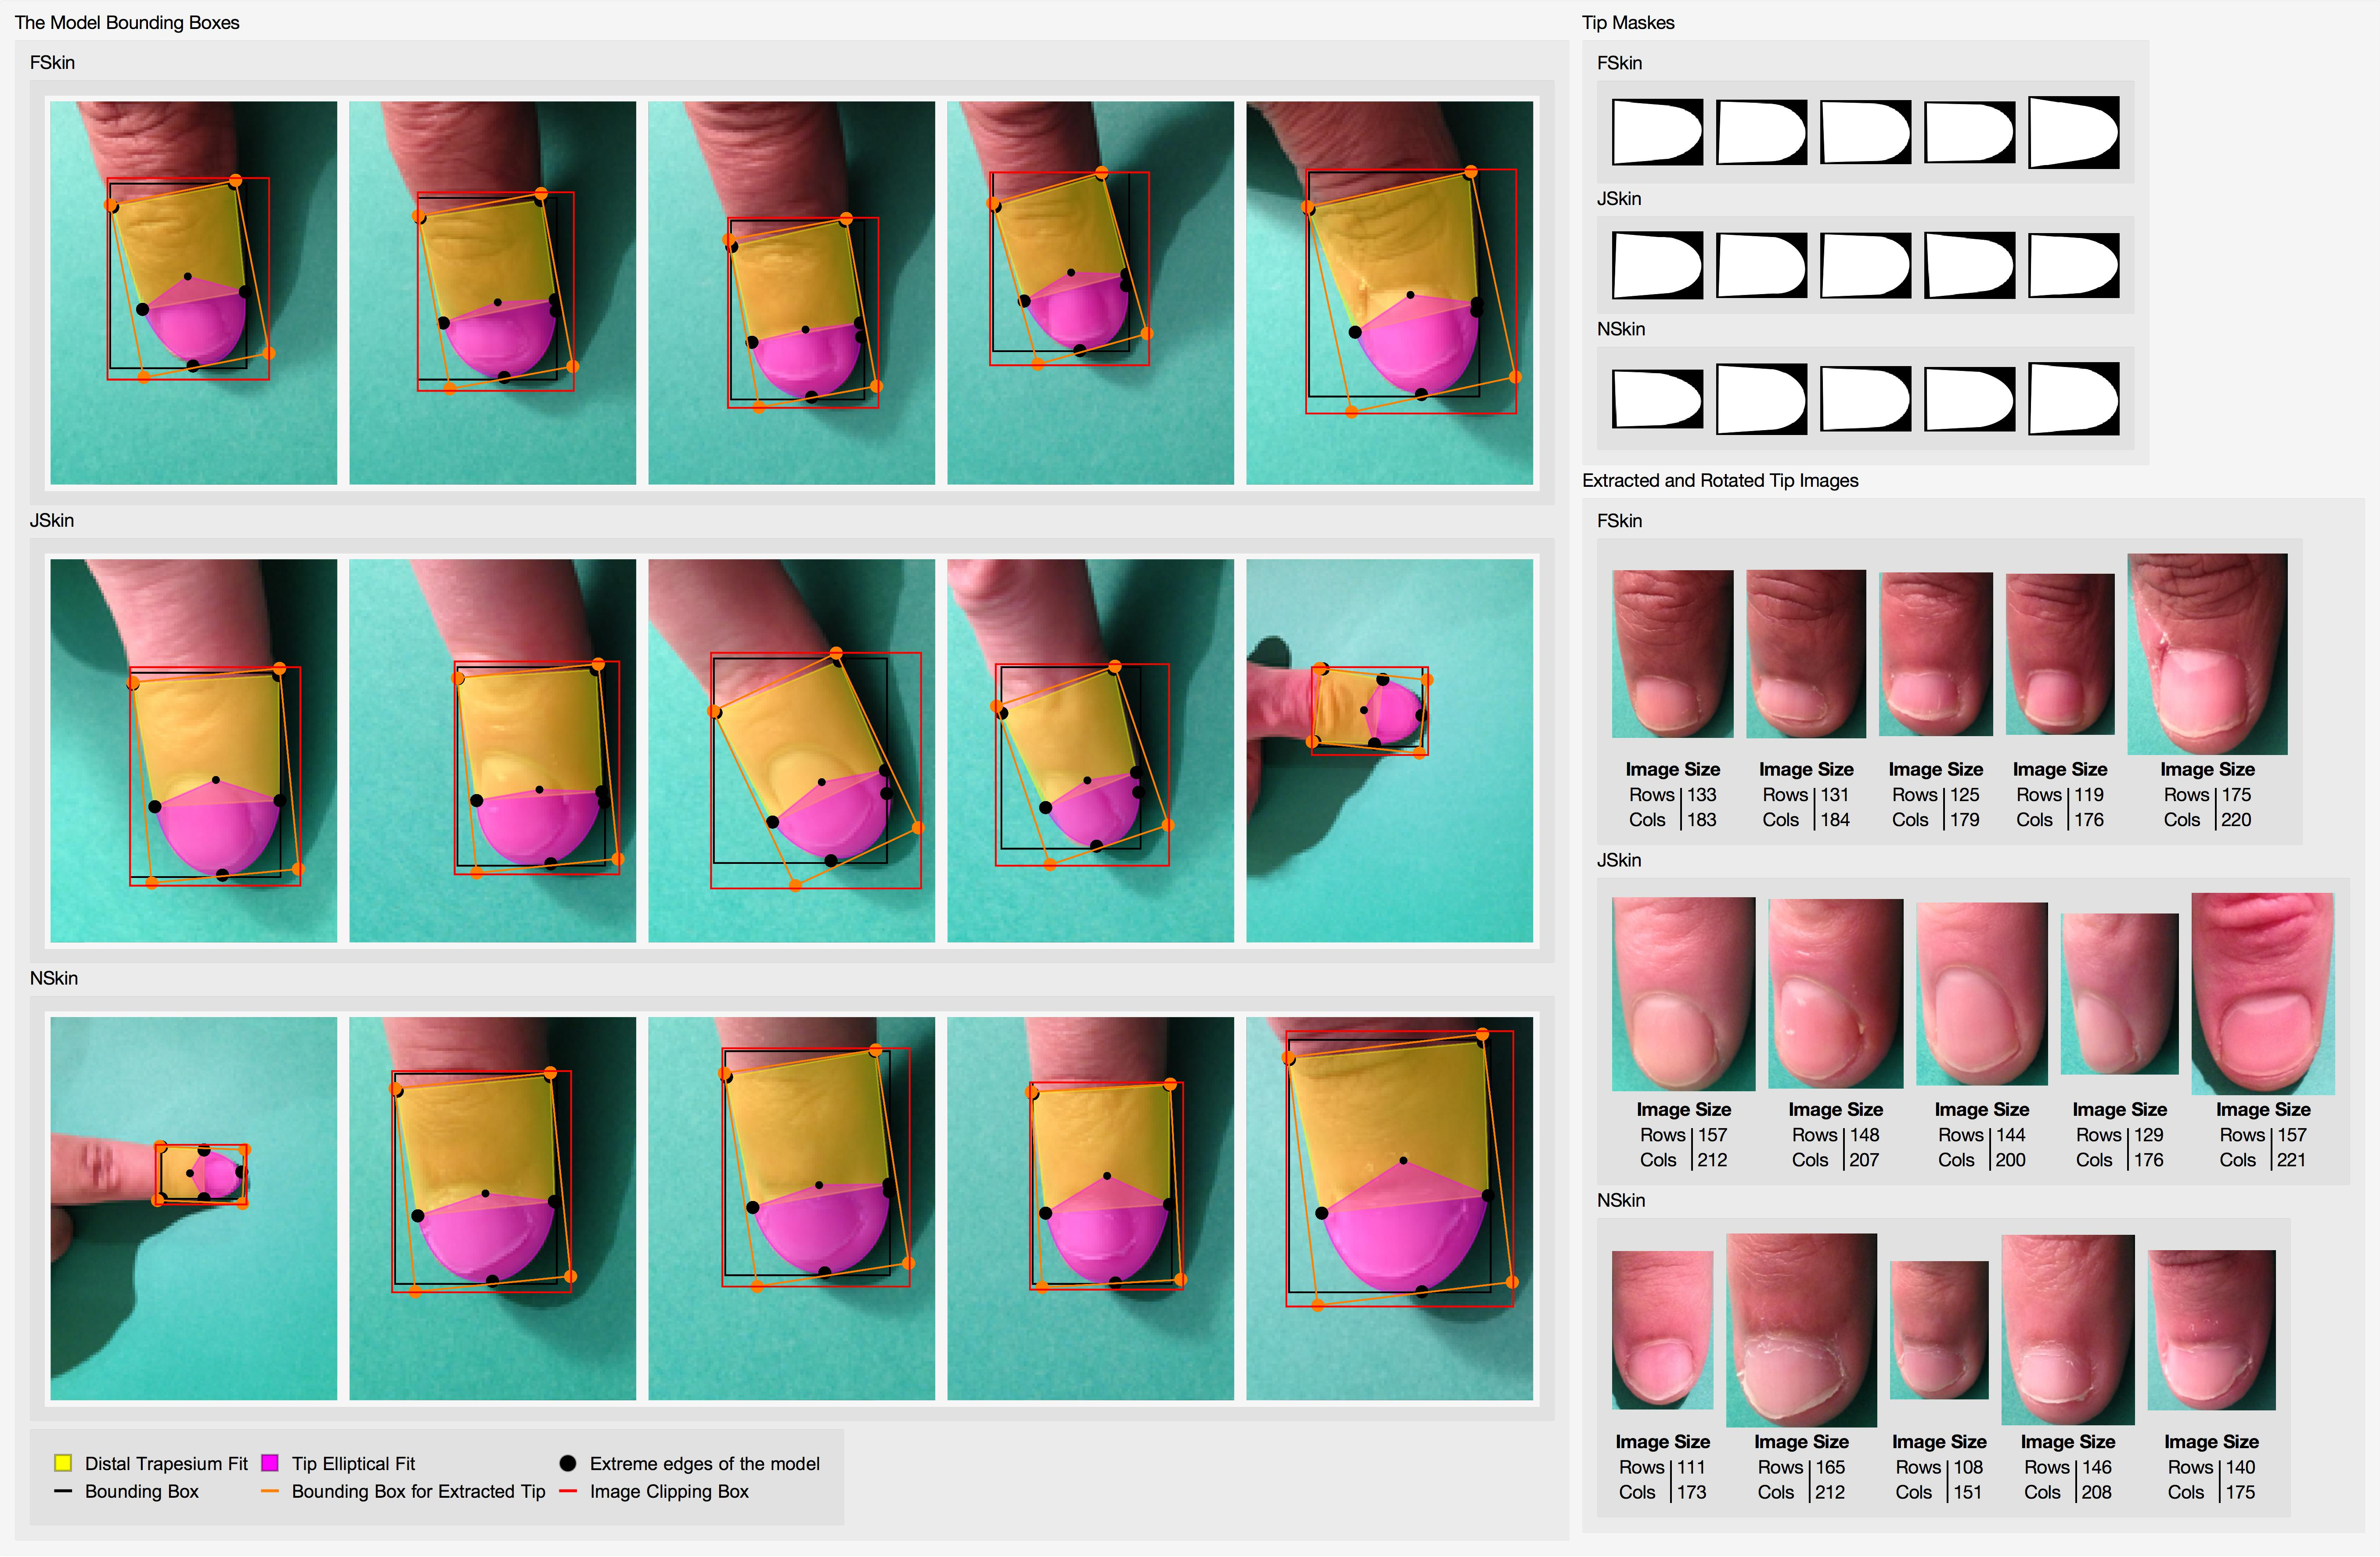
\includegraphics[width=0.95\textwidth]{Chapter4/Figs/Model_Overlayed_Boundary_with_Tips.jpg}
    \caption{The models and model boundaries overlayed on the source images. With tip masks and extracted tip images.}\label{fig:ModelOverlayedBoundaryWithTips}
\end{sidewaysfigure}


\clearpage
\section{Dynamic Tracking}\label{sec:DynamicTracking}
The main purpose of the dynamic tracking algorithm is to categorize the motion of the digit in the frame as "rapid motion," "smooth motion," and "in contact with a surface."

\begin{itemize}
\item \textbf{Rapid motion} --- When the digit is being moved into the frame, or is moving rapidly across the frame, or when the camera is being put into position, it is pointless to attempt to detect a fingertip as this information will quickly become irrelevant. Standard motion detection library routines can be used here on the unaltered video feed. When these algorithms detect motion above a certain threshold, the algorithm does nothing and waits for the motion detected to fall below this threshold.
\item \textbf{Smooth motion} --- Smooth motion is when the digit is being moved in a controlled manner within the frame. When the digit is moving in such a way, it is reasonable to assume that a finger press is imminent. The algorithm takes a frame in the small scale space and processes it into a pixel-categorized image as in Section \ref{sec:QuaternaryPixelClassification}. The frame orientation and digit tip selection are found as in Sections \ref{sec:FindingTheFrameOrientation} and \ref{sec:FindingTheEndOfTheFingerShape}, and then a Filament fill of only the tip is performed similar to Sections \ref{sec:FilamentFill} and \ref{sec:FilamentFillTheFinger}, but now with the Filament fill path being shortened to the length of the distal section in the model. The position and orientation for the model are obtained using the Force Analogue Shape Detection algorithm outlined below, in Section \ref{sec:ForceAnalogue}. The algorithm continues tracking until the change in the position of the tip between successive frames falls below a threshold, at which point the algorithm decides that the digit is likely in contact with a surface, and control passes to the "in contact with a surface" part of the algorithm.
\item \textbf{In contact with a surface (ICWaS)} --- When the tip of the digit is relatively immobile, the digit is likely in contact with a surface; we now want to observe the blood flow. The frame is now captured in the medium space, and is cropped to the edges of the model in its current position and orientation. The cropped image is put into the skin color-space, and a gradient filter is applied to the grayscale channel. If this is the first iteration, this gradient-filtered image is stored; if it is a subsequent iteration, this gradient filter is compared with the first and an alignment transform is found between the current frame and the first frame. To improve the accuracy and avoid the algorithm being distracted by movements at the edge of the digit, the gradient-filtered images are masked with the model, which removes edge-related gradient features, focusing the algorithm on the nail, which is stable during a finger press. The transform is applied to the two chromatic channels, which aligns the images, and the difference is found between successive frames; this gives us the blood flow. 
\end{itemize}

\subsection{Rapid Motion Tracking}\label{sec:RapidMotionTracking}
Before any fingertip tracking is performed, the algorithm checks to see if the digit is still in motion. This is done by first taking the difference between subsequent grayscaled frames from the raw video feed using OpenCV's `absdiff' method. To account for changes in lighting and contrast, a binary threshold is applied to the frames, after which an erosion operation (the `erode' method) is performed to further reduce artifacts and false positives. If the number of changes in the image is above a given threshold, then the digit is considered to be in rapid motion.


\subsection{Smooth Motion Tracking}\label{sec:SmoothMotionTracking}

The find-tip algorithm (Section \ref{sec:FindingTheEndOfTheFingerShape}) gives us a path which we know lies on a digit. This path, however, is not necessarily particularly well-aligned with the axis of the digit. For this reason, we don't ask for a shortened path from the tip to $1 \frac{1}{2}$ distal widths along that path; such a path might actually end closer to the tip than desired, as the path isn't necessarily along the axis. To account for this, we ask for two distal widths from the tip. 

The next problem to be addressed results from the operation of the Filament fill method; because the digit isn't necessarily presented perpendicularly to the frame edge and the Filament fill algorithm finds points perpendicular to the frame edge, we adjust by half the gradient of the path, similarly to the method used in the fingertip model algorithm illustrated in Figure \ref{fig:ModelingFingertip}. So, Filament fill is run along the find-tip path from the tip to a distance of $(2+\left\lvert\frac{1}{2}\delta path\right\lvert)w$ from the tip. This gives us three sets of points: the top, middle and bottom edges, which definitely include points relating to the tip of the digit.

Now we refine these points; because we know the orientation of the frame, we can determine which points correspond to the top edge of the digit, and which points correspond to the bottom. We now put them into standard orientation as in steps a and b in Figure \ref{fig:ModelingFingertip}. 

We now need to find points on the model which would ideally correspond with the points found by Filament fill in the image. First, we need to obtain a reasonably good measure of the orientation of the digit; given that we have midline points on the digit which reasonably correspond to the distal segment, a linear fit to the middle $\frac{2}{3}$ of these points provides a good measure of the orientation with little computational cost. Rather than reorientating the image points to a neutral coordinates, we rotate the model to correspond with the image coordinates. This is easily achieved as the model is centered on the ellipse, and so involves a rotation of the four points of the trapezian and adding the rotation to the ellipse's orientation.

In the model's new orientation, we find the furthest point on the model in the $x$ axis. (It should be noted that this is not necessarily what we would refer to as the "tip" of the digit.) We assume that this point on the model corresponds to the first point in the midline set of points; the Filament fill follows the path from the tip back to the frame edge, so the first point in the midline should be the tip. So, we create a set of $x$ axis coordinates where the first midline point corresponds with the furthest point on the model in the $x$ axis. We do this because the Filament fill divides up the shape vertically in a relatively regular fashion, so we are dividing up the model in the way that we would expect Filament fill to if the model were an image. This allows us to put points on the model and points in the image into a $1:1$ correspondence. So although the fingertip model is a relatively arbitrary geometric shape, the regularity of the Filament fill method allows us to use a force analogue shape detection algorithm as outlined previously (Section \ref{sec:ForceAnalogue}).

\begin{figure}[h!]
  \centering
    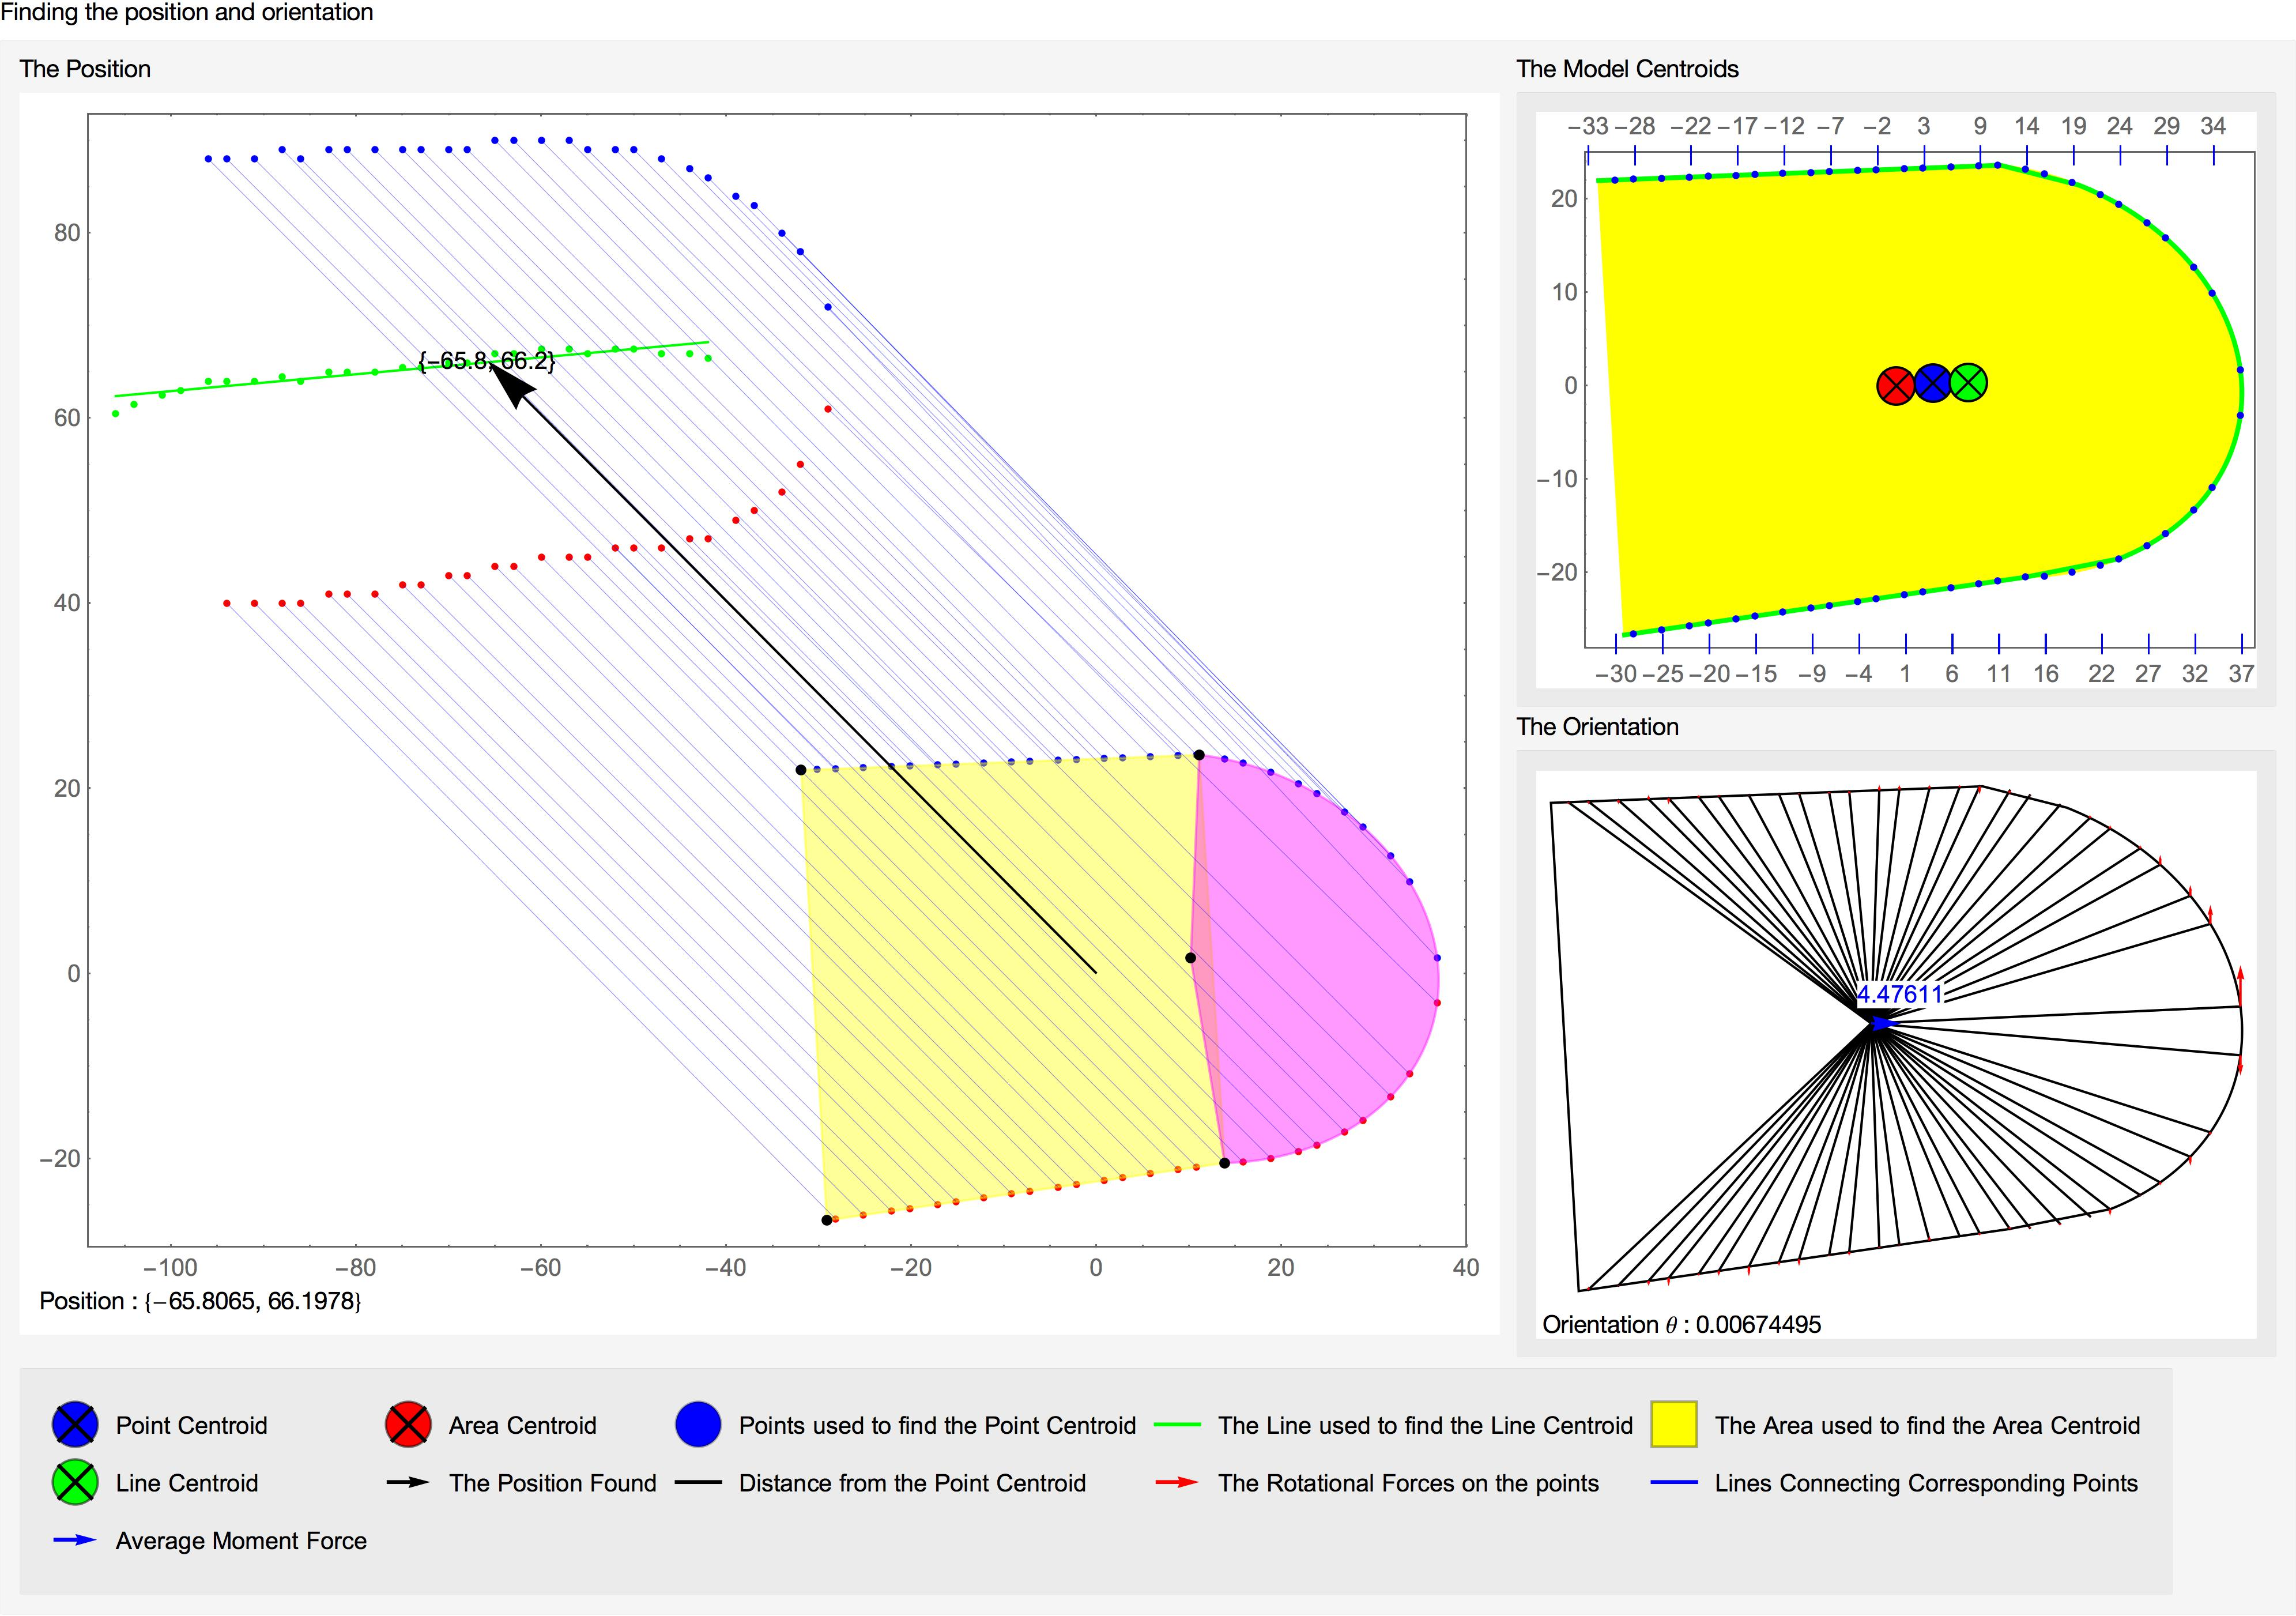
\includegraphics[width=0.95\textwidth]{Chapter4/Figs/Model_Centroids_With_Pos_Orientation.jpg}
    \caption{Finding the Position and Orientation of the Tip. A side-effect of the pre-alignment of the model means that, almost always,  the change in the orientation from the force analogue shape detection algorithm is negligible. }\label{fig:PositionAndOrientation}
\end{figure}

A side-effect of the pre-alignment of the model means that --- almost always --- the change in the orientation from the force analogue shape detection algorithm is negligible.

The distribution of points around the perimeter of the model is dependant on the orientation of the digit in the image. This means that the point centroid is not constant, and so a shape-based area centroid is used in the modeling stage (Figure \ref{fig:PositionAndOrientation}). 

\begin{figure}[h!]
  \centering
    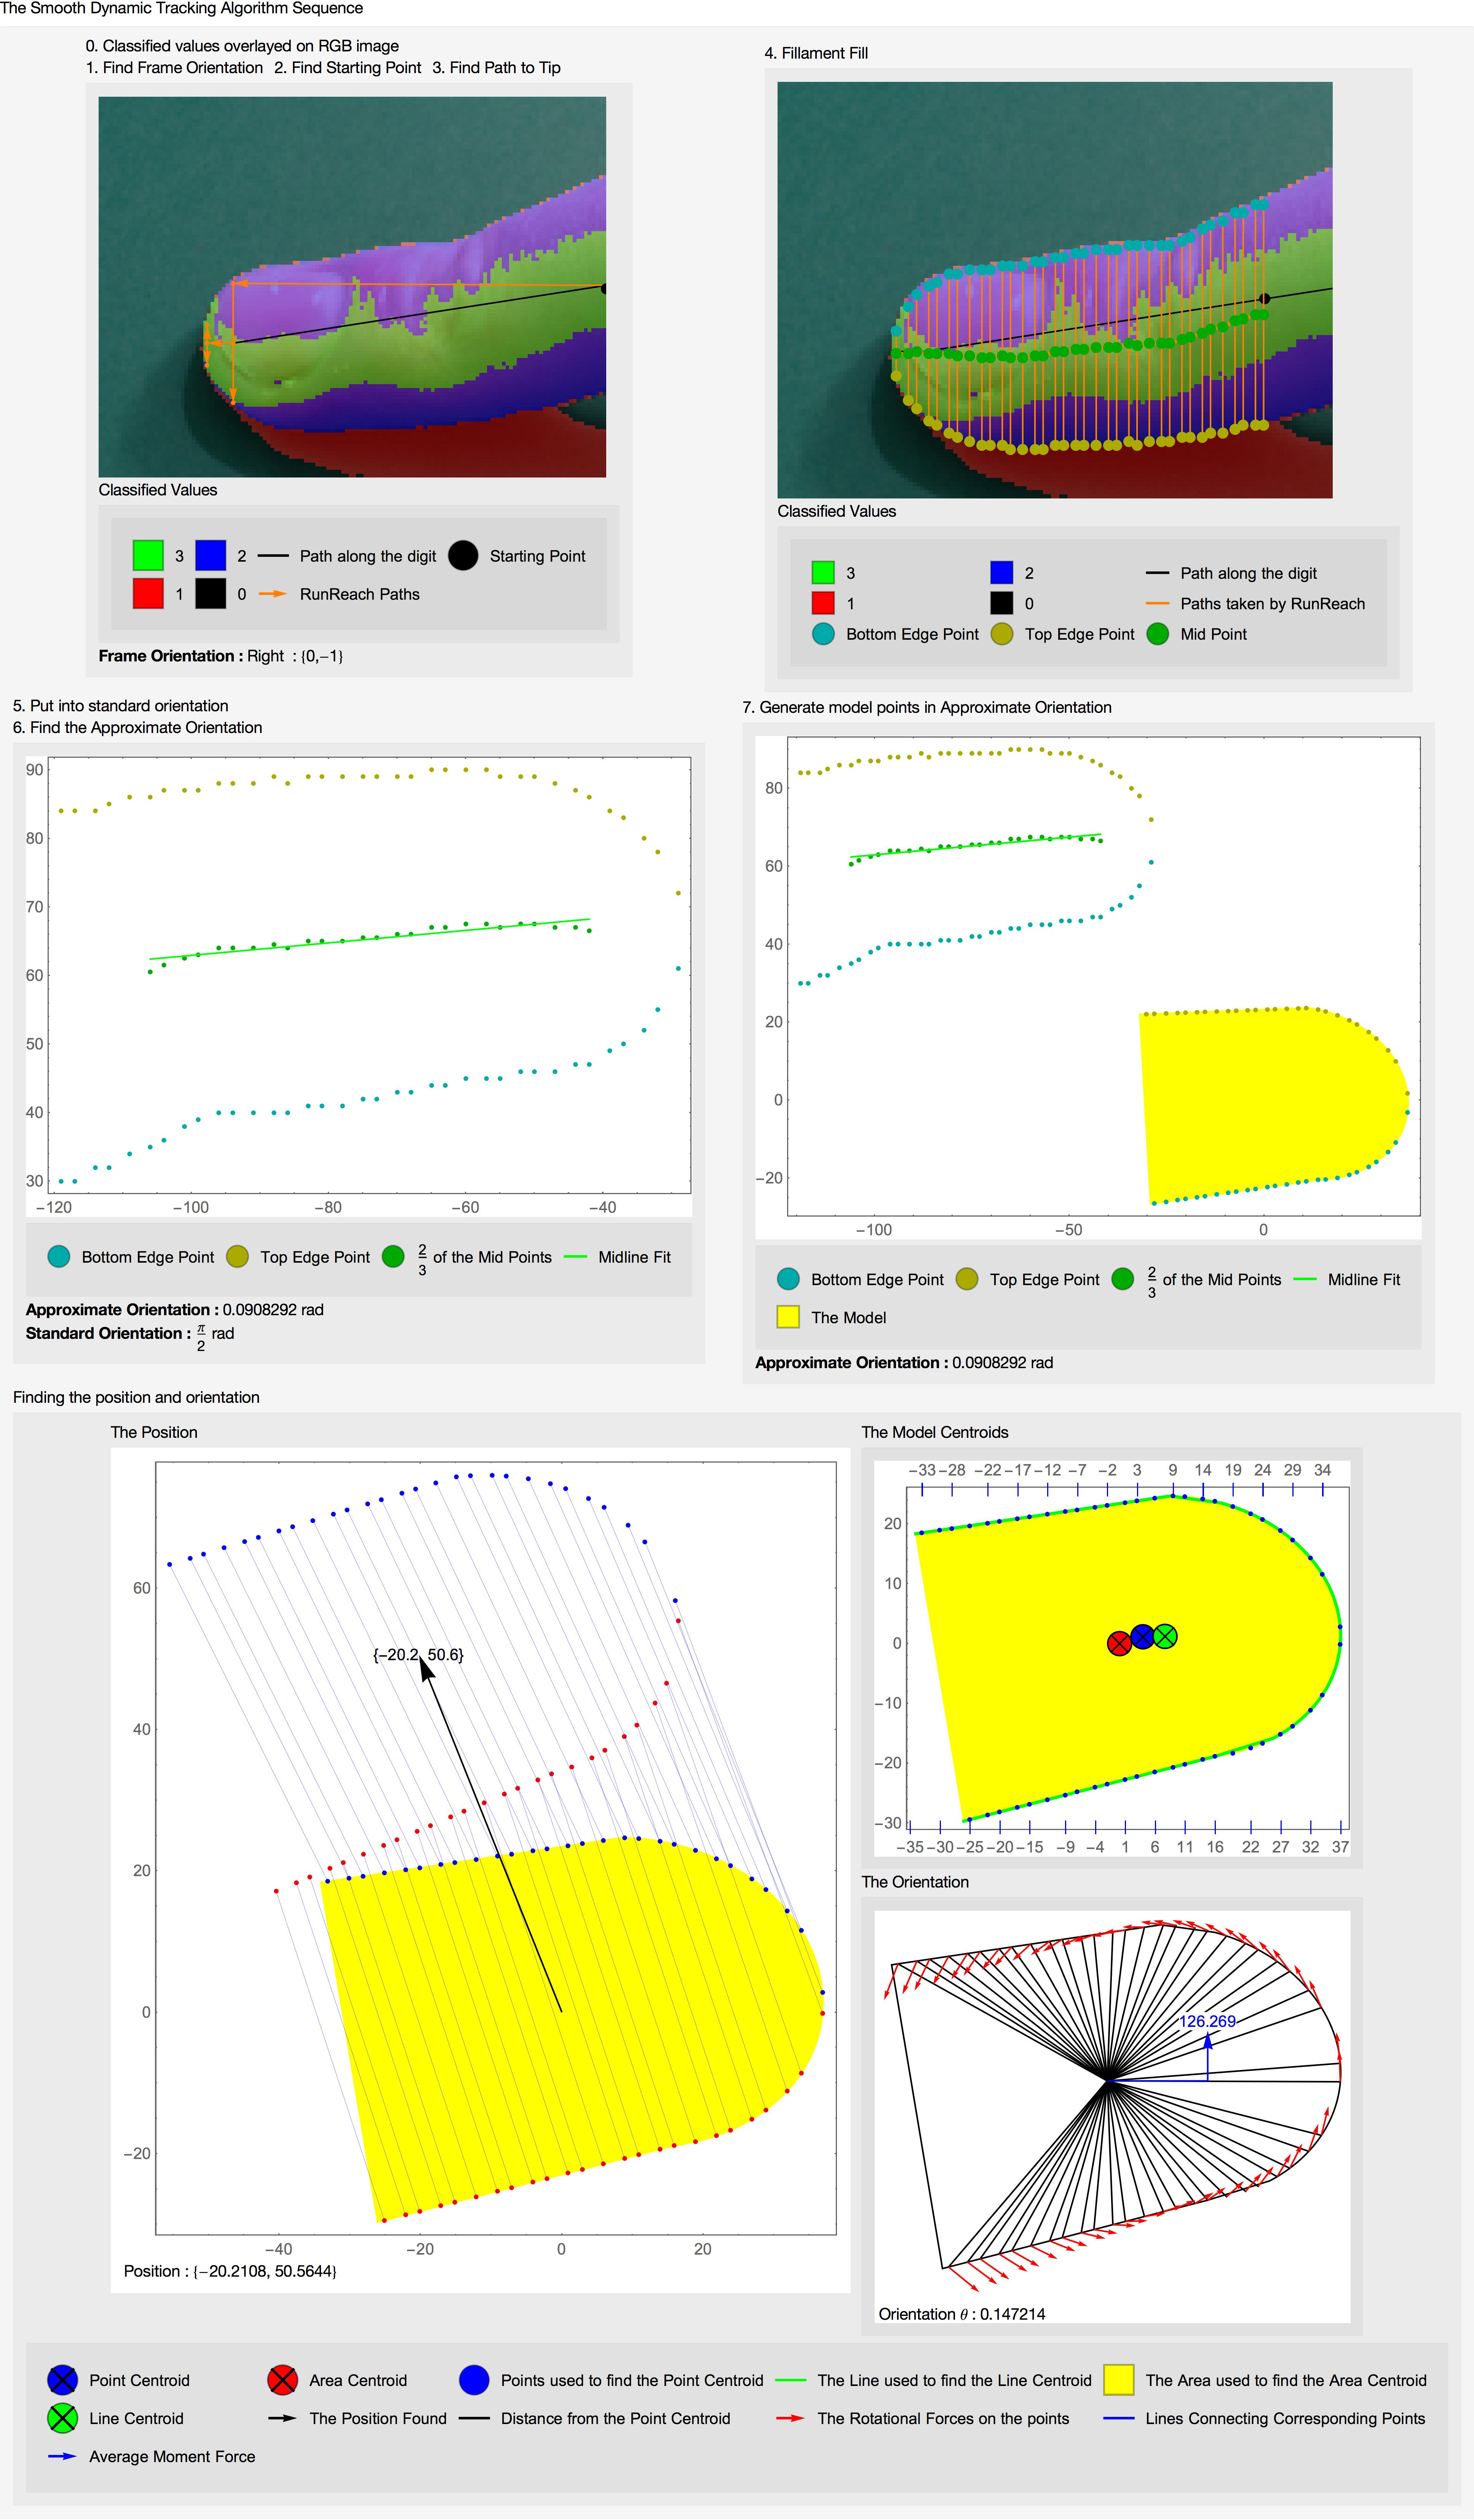
\includegraphics[width=0.85\textwidth]{Chapter4/Figs/Smooth_Dynamic_Sequence.jpg}
    \caption{Smooth Dynamic Sequence}\label{fig:SmoothDynamicSequence}
\end{figure}


In practice, the algorithm first finds the rough orientation of the digit in the image and rotates the model accordingly. The model is re-centered on the point centroid for the current orientation before the FASDM method is used. 

In addition to the FASDM method, the algorithm also finds the mean of the length of the vectors between the rotated and translated model points and the points on the image. To be clear, this distance is signed according to which point is further away from the model center. This allows the model to be scaled. The upshot of this is that the code correctly follows a digit even as the digit moves closer or further away from the camera. (Fingers do not normally change shape.)
\clearpage
\subsection{ICWaS Method}\label{sec:ICWaS}
The ICWaS method performs three main tasks: cropping the midscale image around the tip; providing a multiplicative mask which highlights blood flow in the tip; and aligning successive frames in-order to find the pixel color differences in the skin color-space. Combining these three tasks allows the blood flow to be shown.

\subsubsection{ICWaS Setup}\label{sec:ICWaSSetup}
From the Smooth Movement Tracking (Section \ref{sec:SmoothMotionTracking}), we have a model position and orientation in the small scale space. We wish to track the blood flow using the medium scale image, so first we must put the model in the medium scale space. This is as simple as multiplying the coordinates by a scaling factor as shown in Section \ref{sec:ScaleSpace}.

Now we want to find the extreme top, bottom, left and right edges of the model in order to crop the midscale image appropriately. The model is comprised of a quadrilateral and an ellipse. To find the extreme edges of the quadrilateral, the algorithm just finds the minimum and maximum values of the coordinates of its vertices. The ellipse's extreme edges can be found using

\begin{minipage}{0.7\textwidth}
\begin{align*}
\begin{array}{ll}
e_1= \Bigg( x_0+\frac{(a-b) (a+b) }{A} \sin \left( \theta \right) & , y_0+A \cos \left( \theta \right) \Bigg)\\
e_2=  \Bigg( x_0-\frac{(a-b) (a+b)}{A} \sin \left( \theta \right) & , y_0-A \cos \left( \theta \right) \Bigg)\\
e_3=  \Bigg( x_0-B \cos \left( \theta \right)  & , y_0-\frac{(a-b) (a+b) }{B} \sin \left( \theta \right) \Bigg)\\
e_4=  \Bigg( x_0+B \cos \left( \theta \right)  & , y_0+\frac{(a-b) (a+b) }{B} \sin \left( \theta \right) \Bigg)\\
\end{array} \\
 \text{where}\quad 
\begin{array}{c}
A=\sqrt{a^2 \tan ^2(\theta )+b^2} \\
B=\sqrt{a^2+b^2 \tan ^2(\theta )} \\
-\frac{\Pi}{2}< \theta < \frac{\Pi}{2}
\end{array}
\end{align*}
\end{minipage}%%%%%%%%%%%%%%%%
\begin{minipage}{0.3\textwidth}
 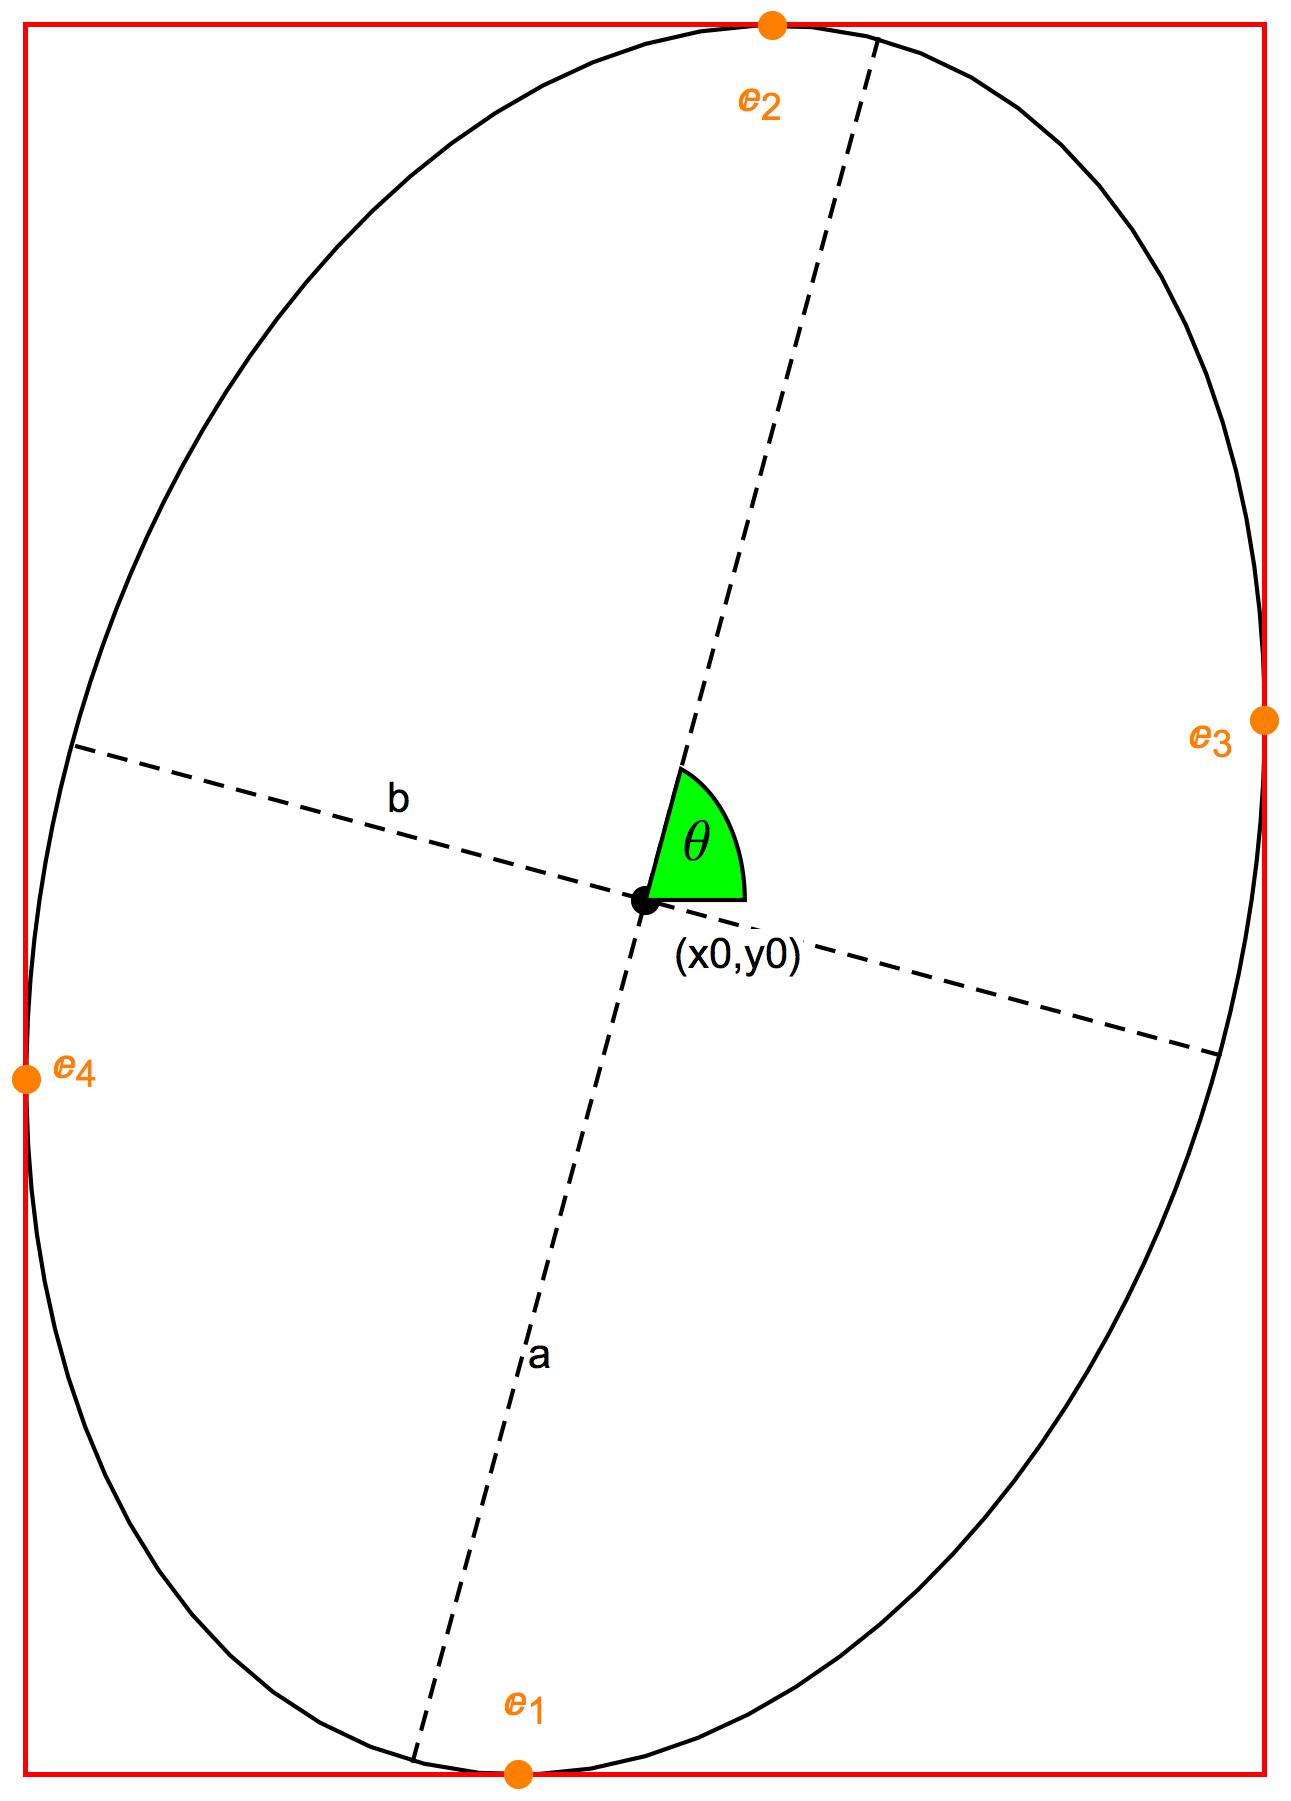
\includegraphics[width=\textwidth]{Chapter4/Figs/Elliptical_Bounds.jpg}
\end{minipage}


However, we only want to include extreme points which lie on the curve which models the tip. The curve which models the tip is the part of the ellipse which falls between the two points on the quadrilateral closest to the tip; we can check if the extreme edges of the ellipse are on this part of the curve by checking that they lie at an angular position between the angles at which the tipmost quadrilateral points lie.

Now we have the extreme edges of the model. These points are used to find a bounding box, which includes all the tip pixels in the small scale space. Translating these to the medium scale space, we subtract the scaling factor from the lower coordinates and add the scaling factor to the higher coordinates, ensuring that the box does not crop any pixels from the digit in the medium scale space. We now take the medium scale RGB image, crop it to the model bounding box, and then pass the extracted tip image to the skin color-space processing routines. The grayscale image is saved as a template for the template matching algorithm.

During a finger press, we expect the flesh to deform around the tip, making the edges of the digit unreliable for alignment, so we wish to construct a binary mask which tells the template matching algorithm which pixels to use for alignment. Using OpenCV's drawing routines, we render the model in the midscale tip image coordinates. This is done in a way which actually renders the model 'slightly' by four or five pixels smaller than the model proper. This effectively eliminates the edge of the digit next to the background, pushing the algorithm to rely on features which do not deform, such as the nail.

\subsubsection{Blood Flow}\label{sec:BloodFlow}

\begin{figure}[h!]
  \centering
    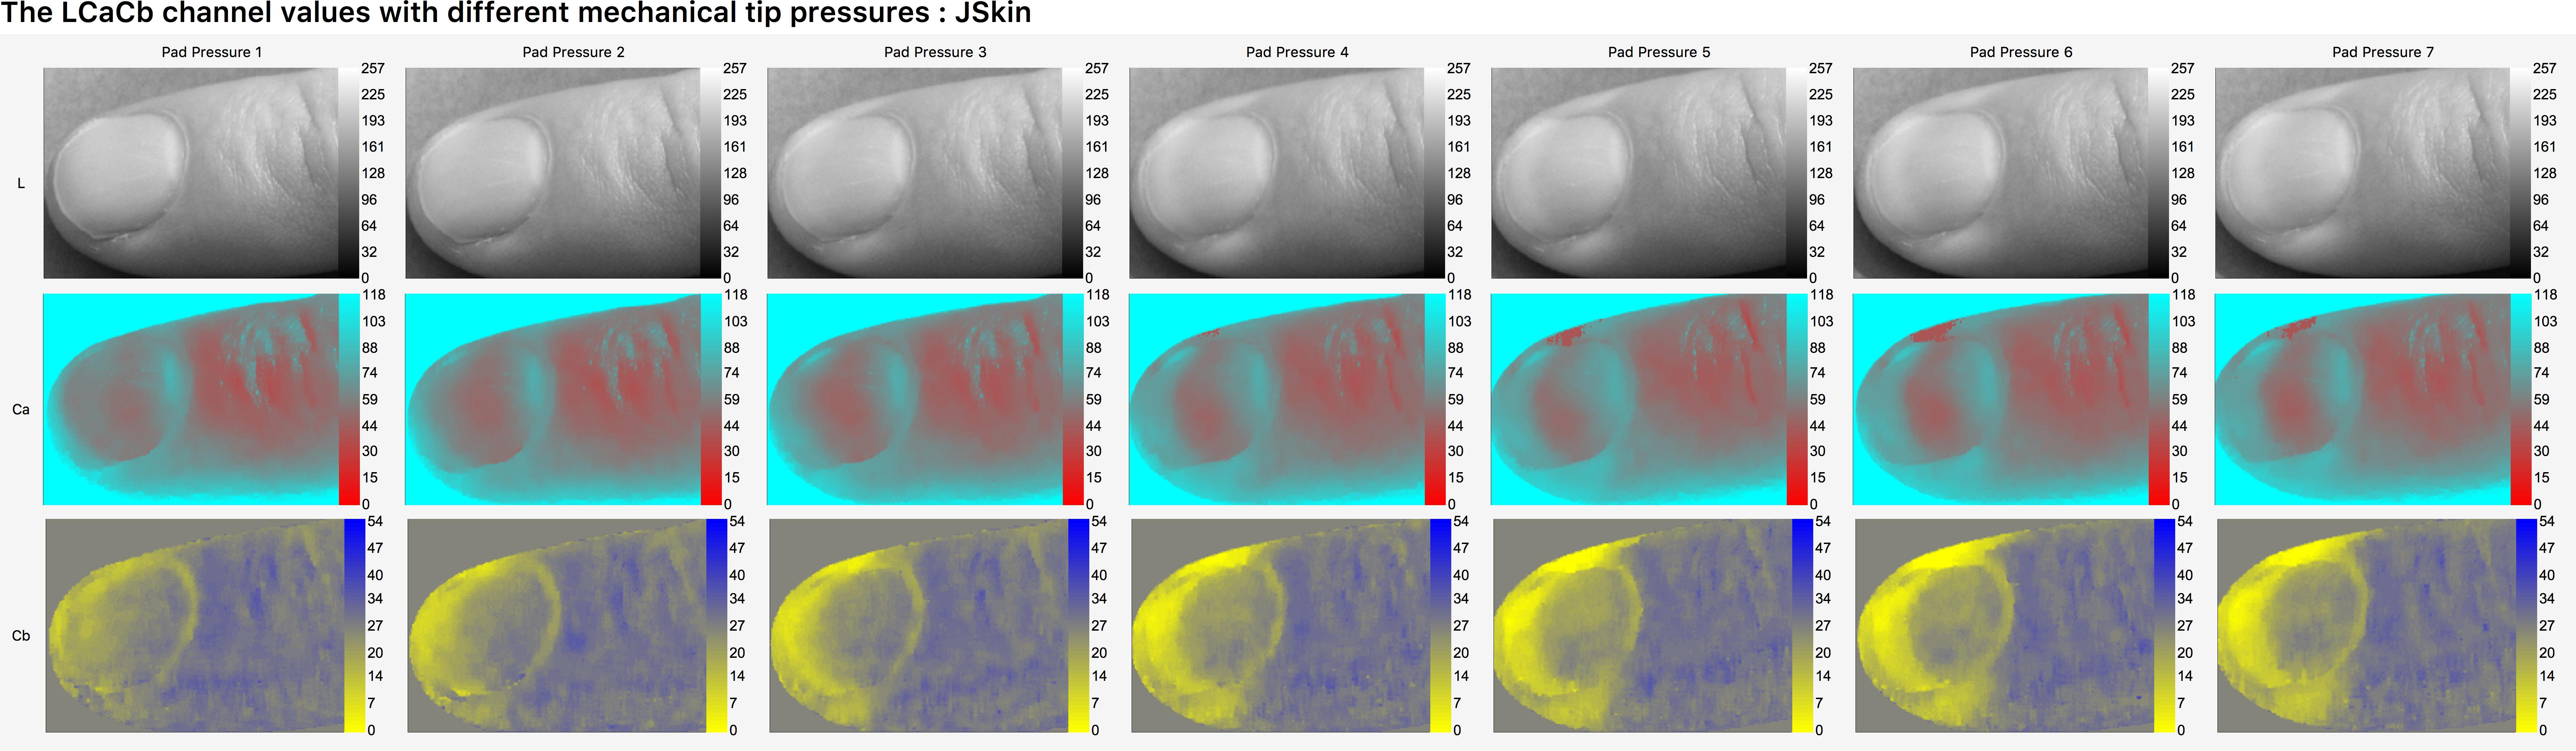
\includegraphics[width=1.00\textwidth]{Chapter4/Figs/Final_Fig_Channels_JSkin.jpg}
%    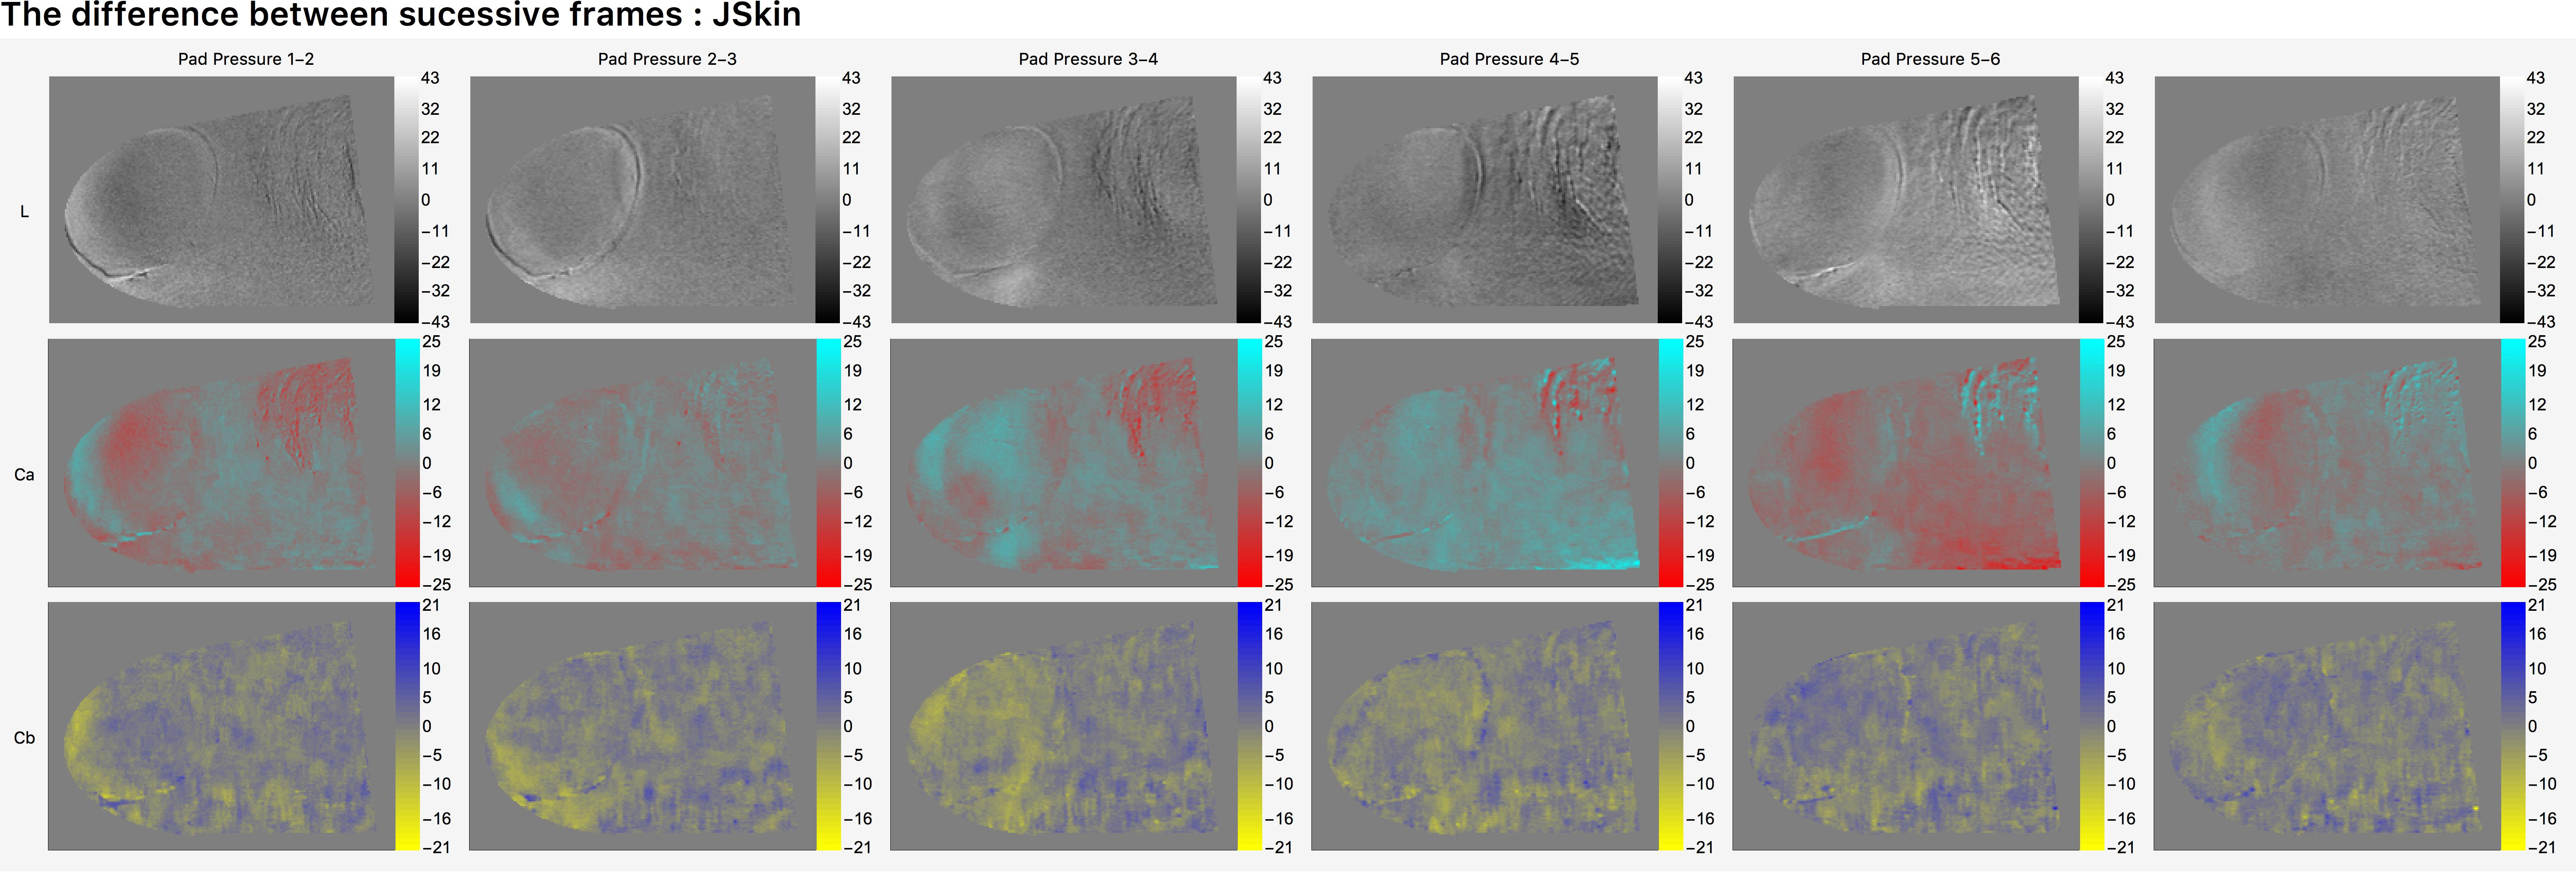
\includegraphics[width=0.86\textwidth]{Chapter4/Figs/Final_Fig_Difference_JSkin.jpg}
    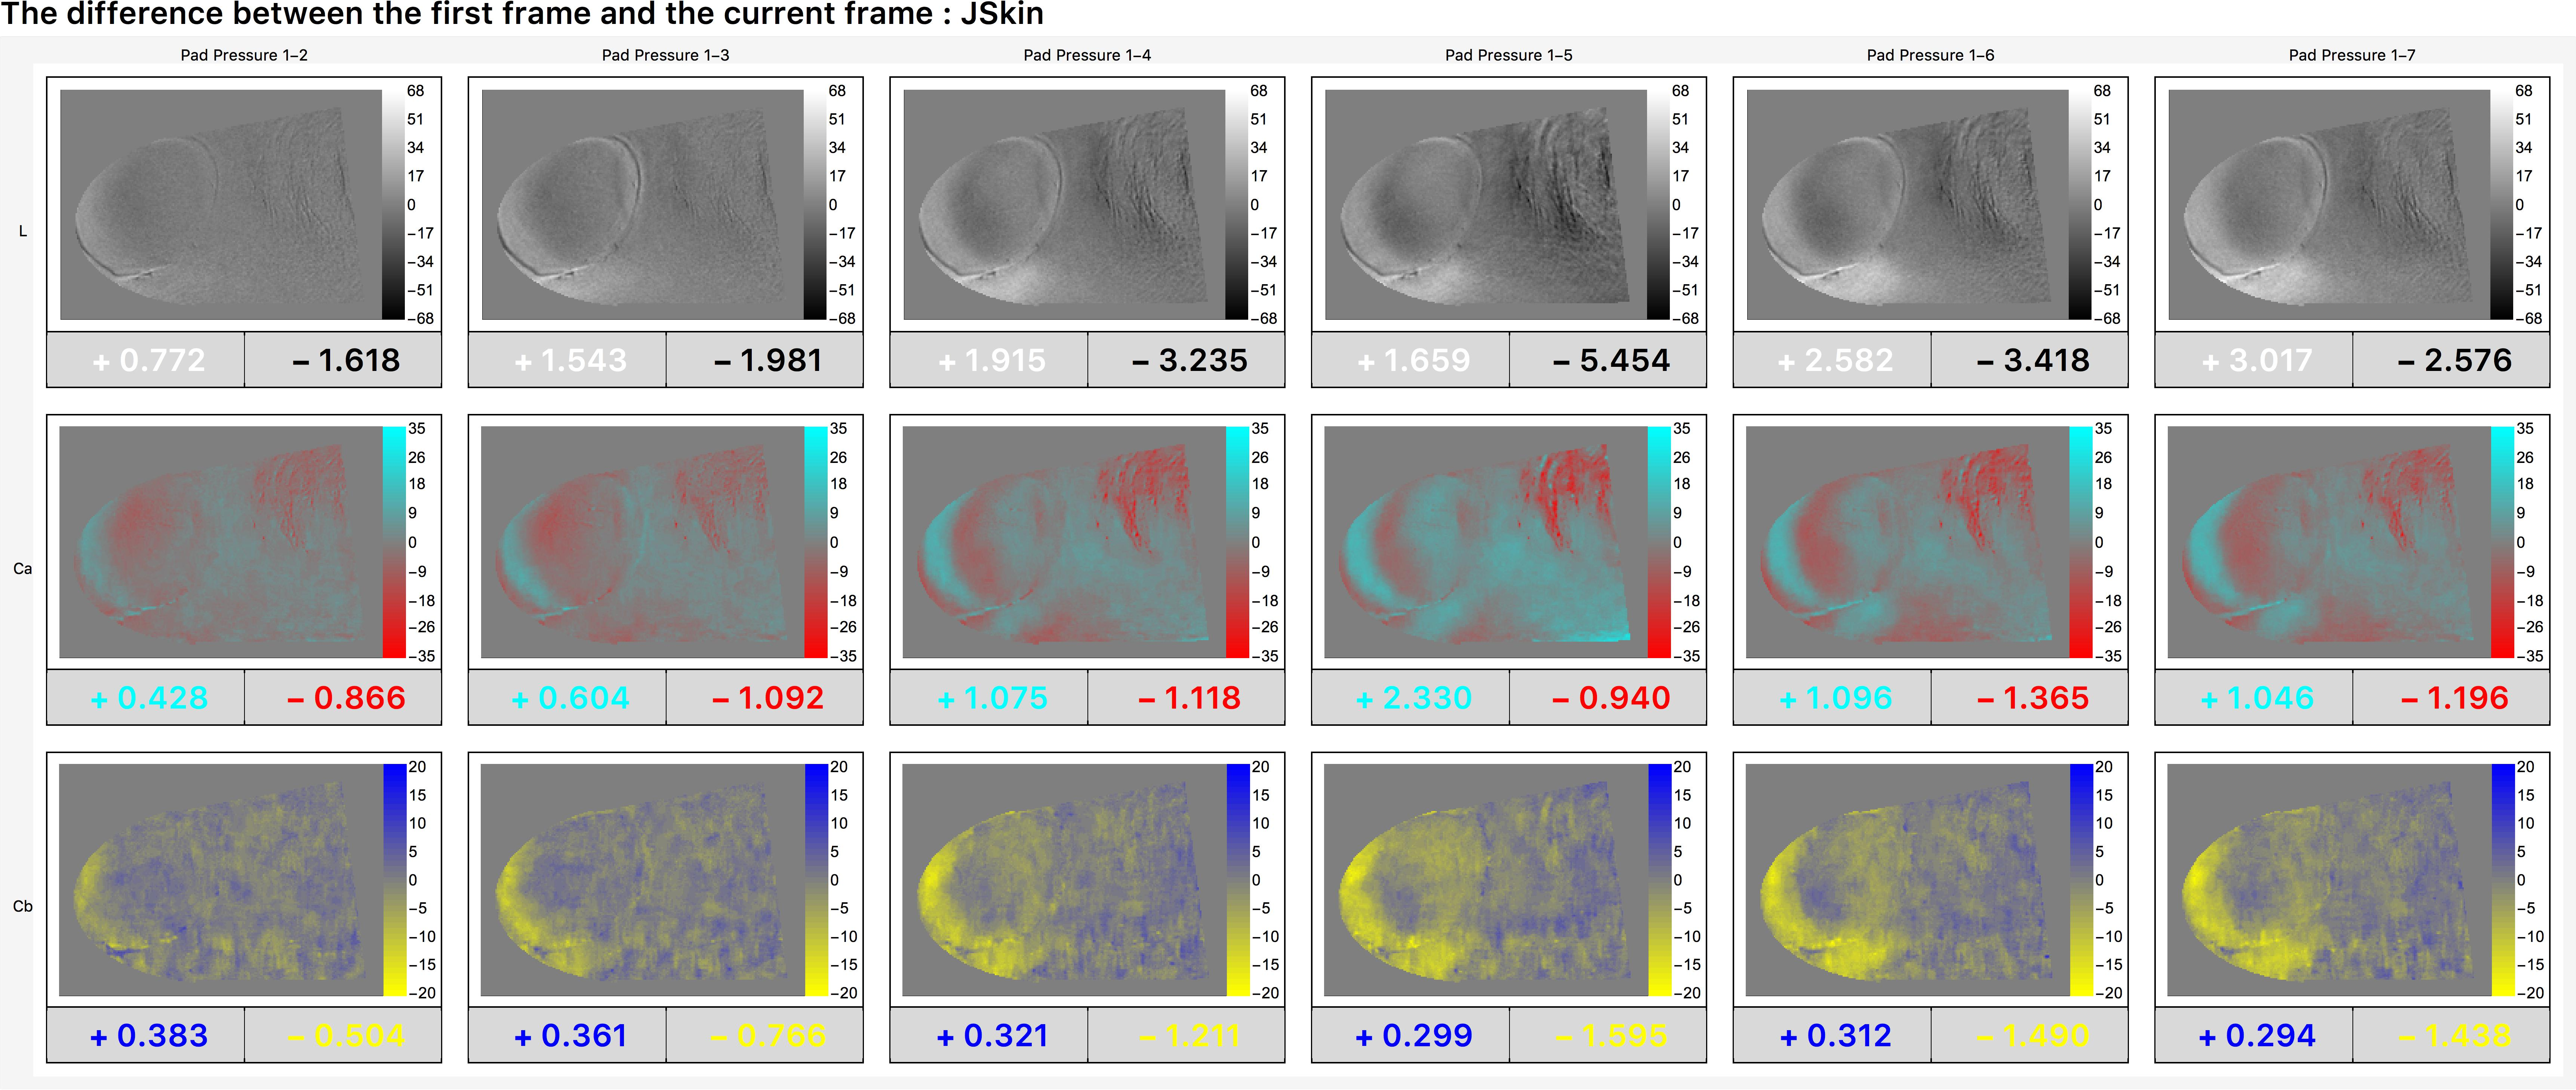
\includegraphics[width=0.86\textwidth]{Chapter4/Figs/Final_Fig_Total_Difference_JSkin.jpg}
    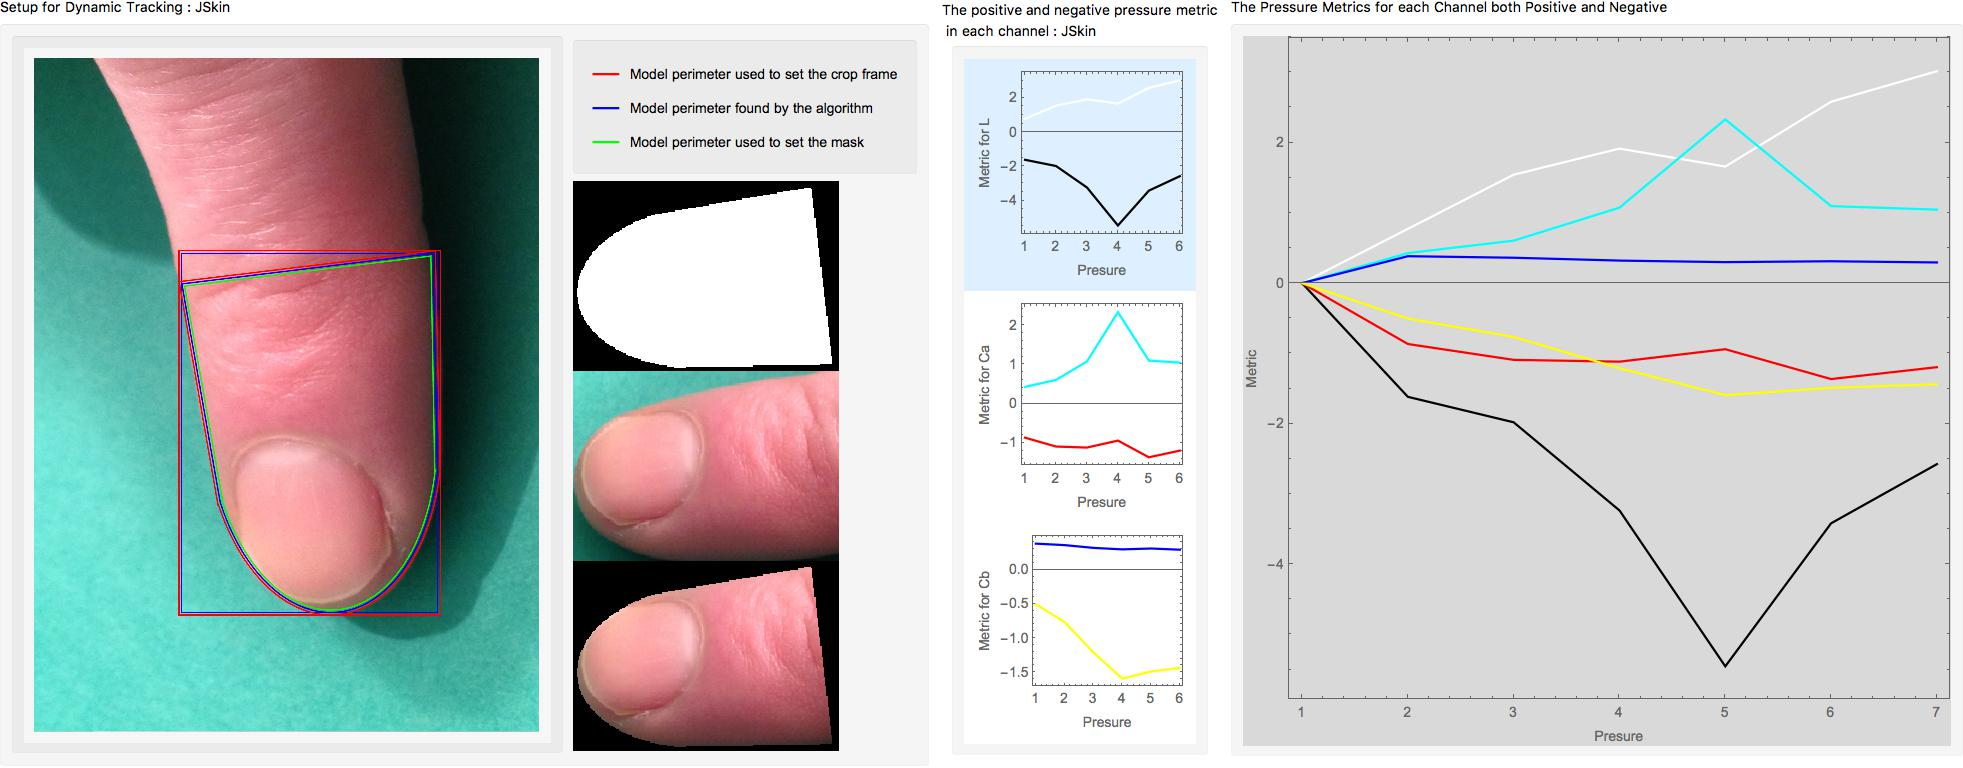
\includegraphics[width=1.00\textwidth]{Chapter4/Figs/Final_Fig_Misc_JSkin.jpg}
    \caption{The resulting sequence of images from the ICWaS algorithm followed by the differences. The metric is the result of summing the positive and negative changes separately and then dividing by the number of pixels. Finally, the initial image of the sequence is shown with the model outline, the slightly larger model used to set the crop frame and the slightly smaller model used for setting the mask.}\label{fig:ICWaSResultJSkin}
\end{figure}

\begin{figure}[h!]
  \centering
    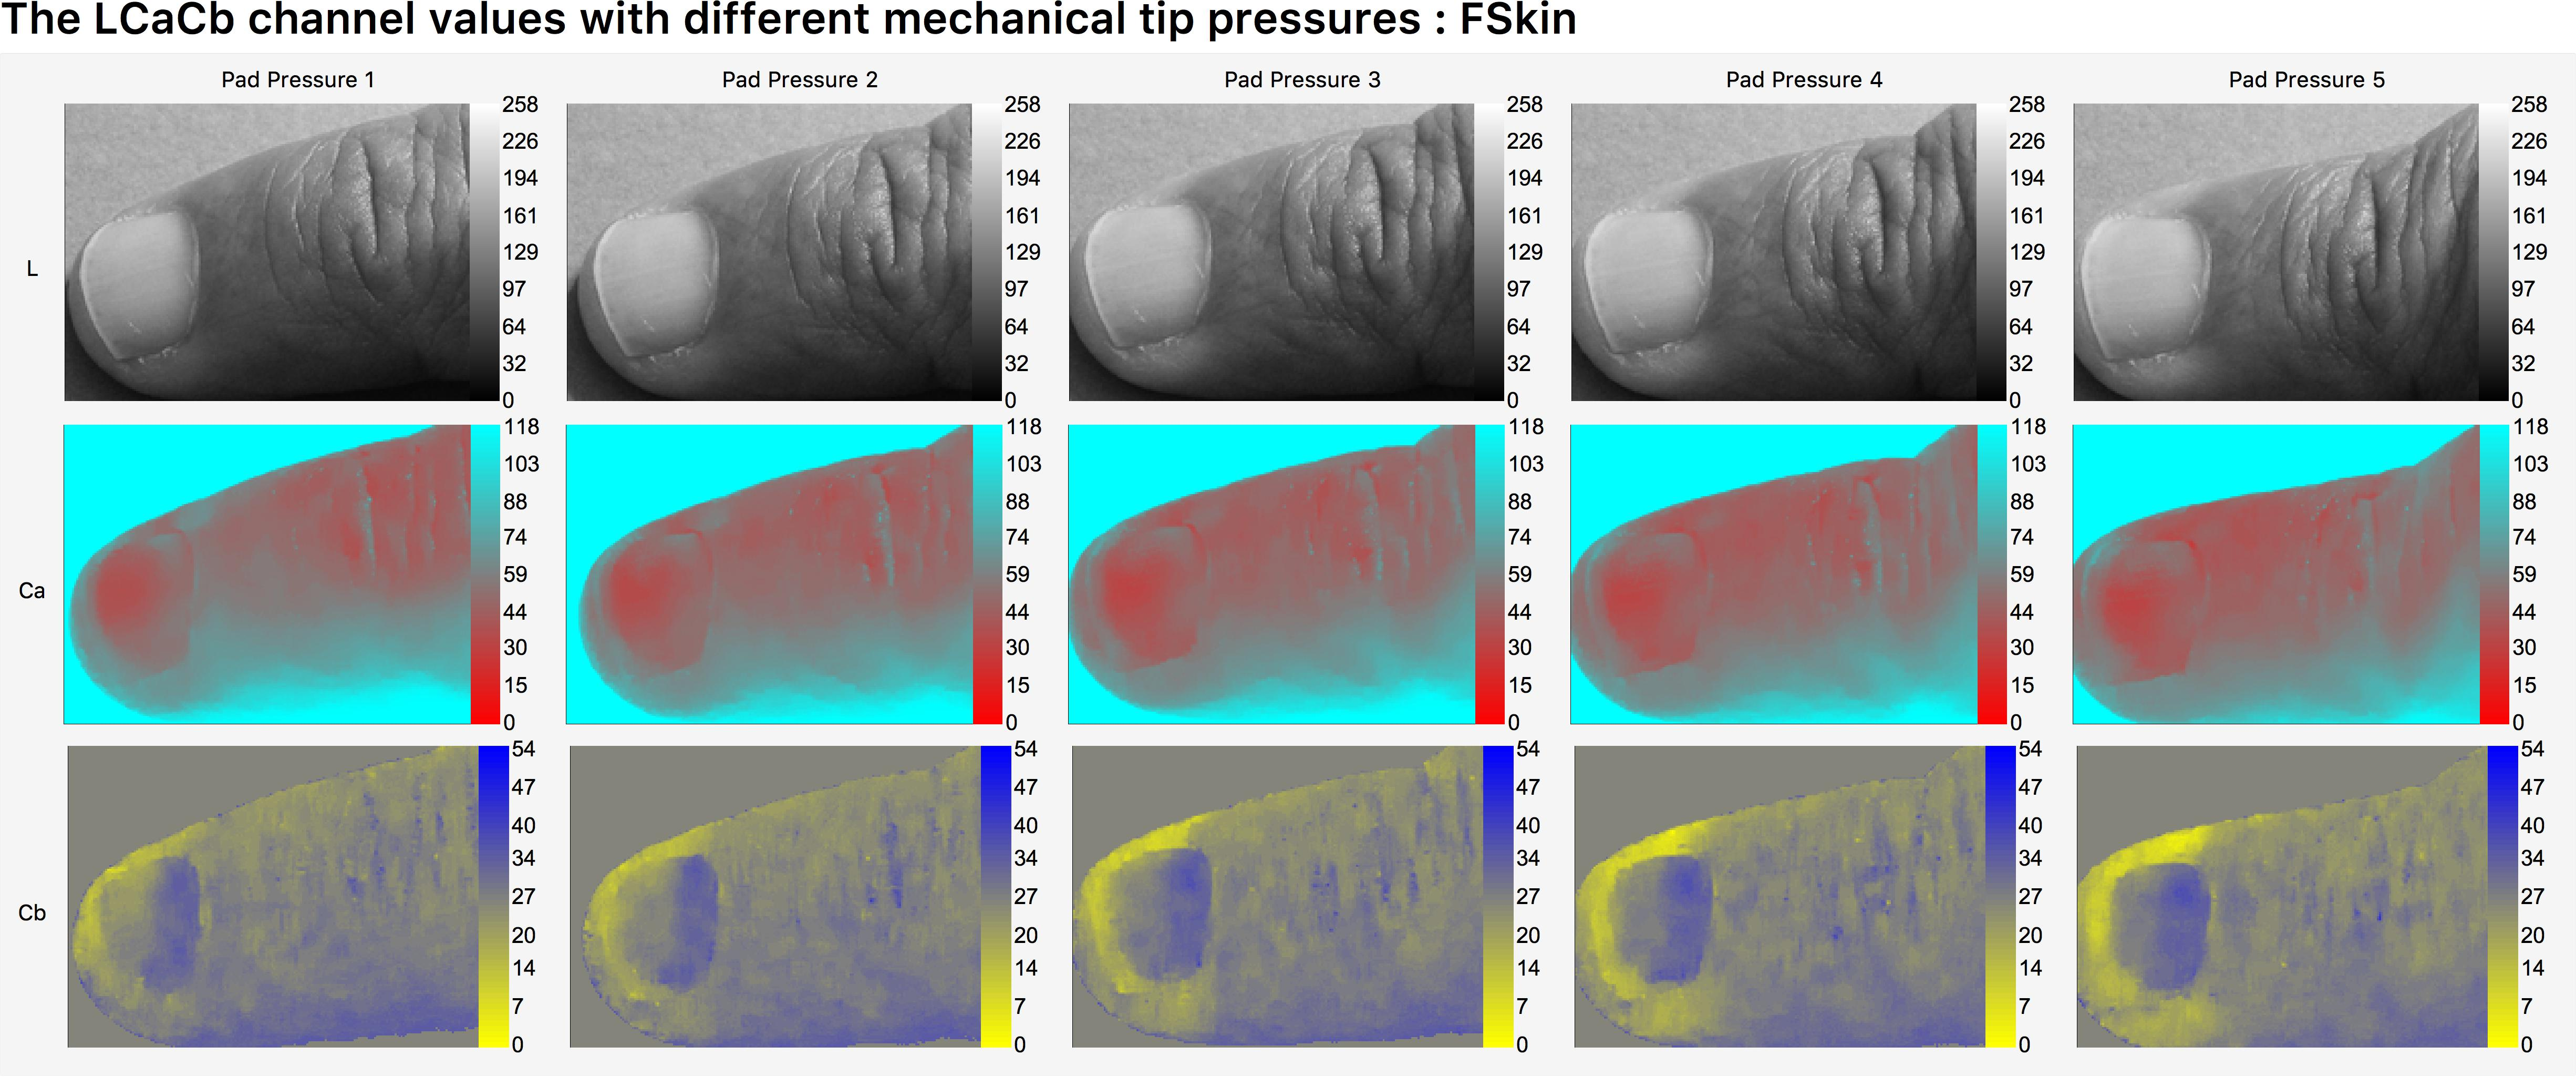
\includegraphics[width=0.820\textwidth]{Chapter4/Figs/Final_Fig_Channels_FSkin.jpg}
%    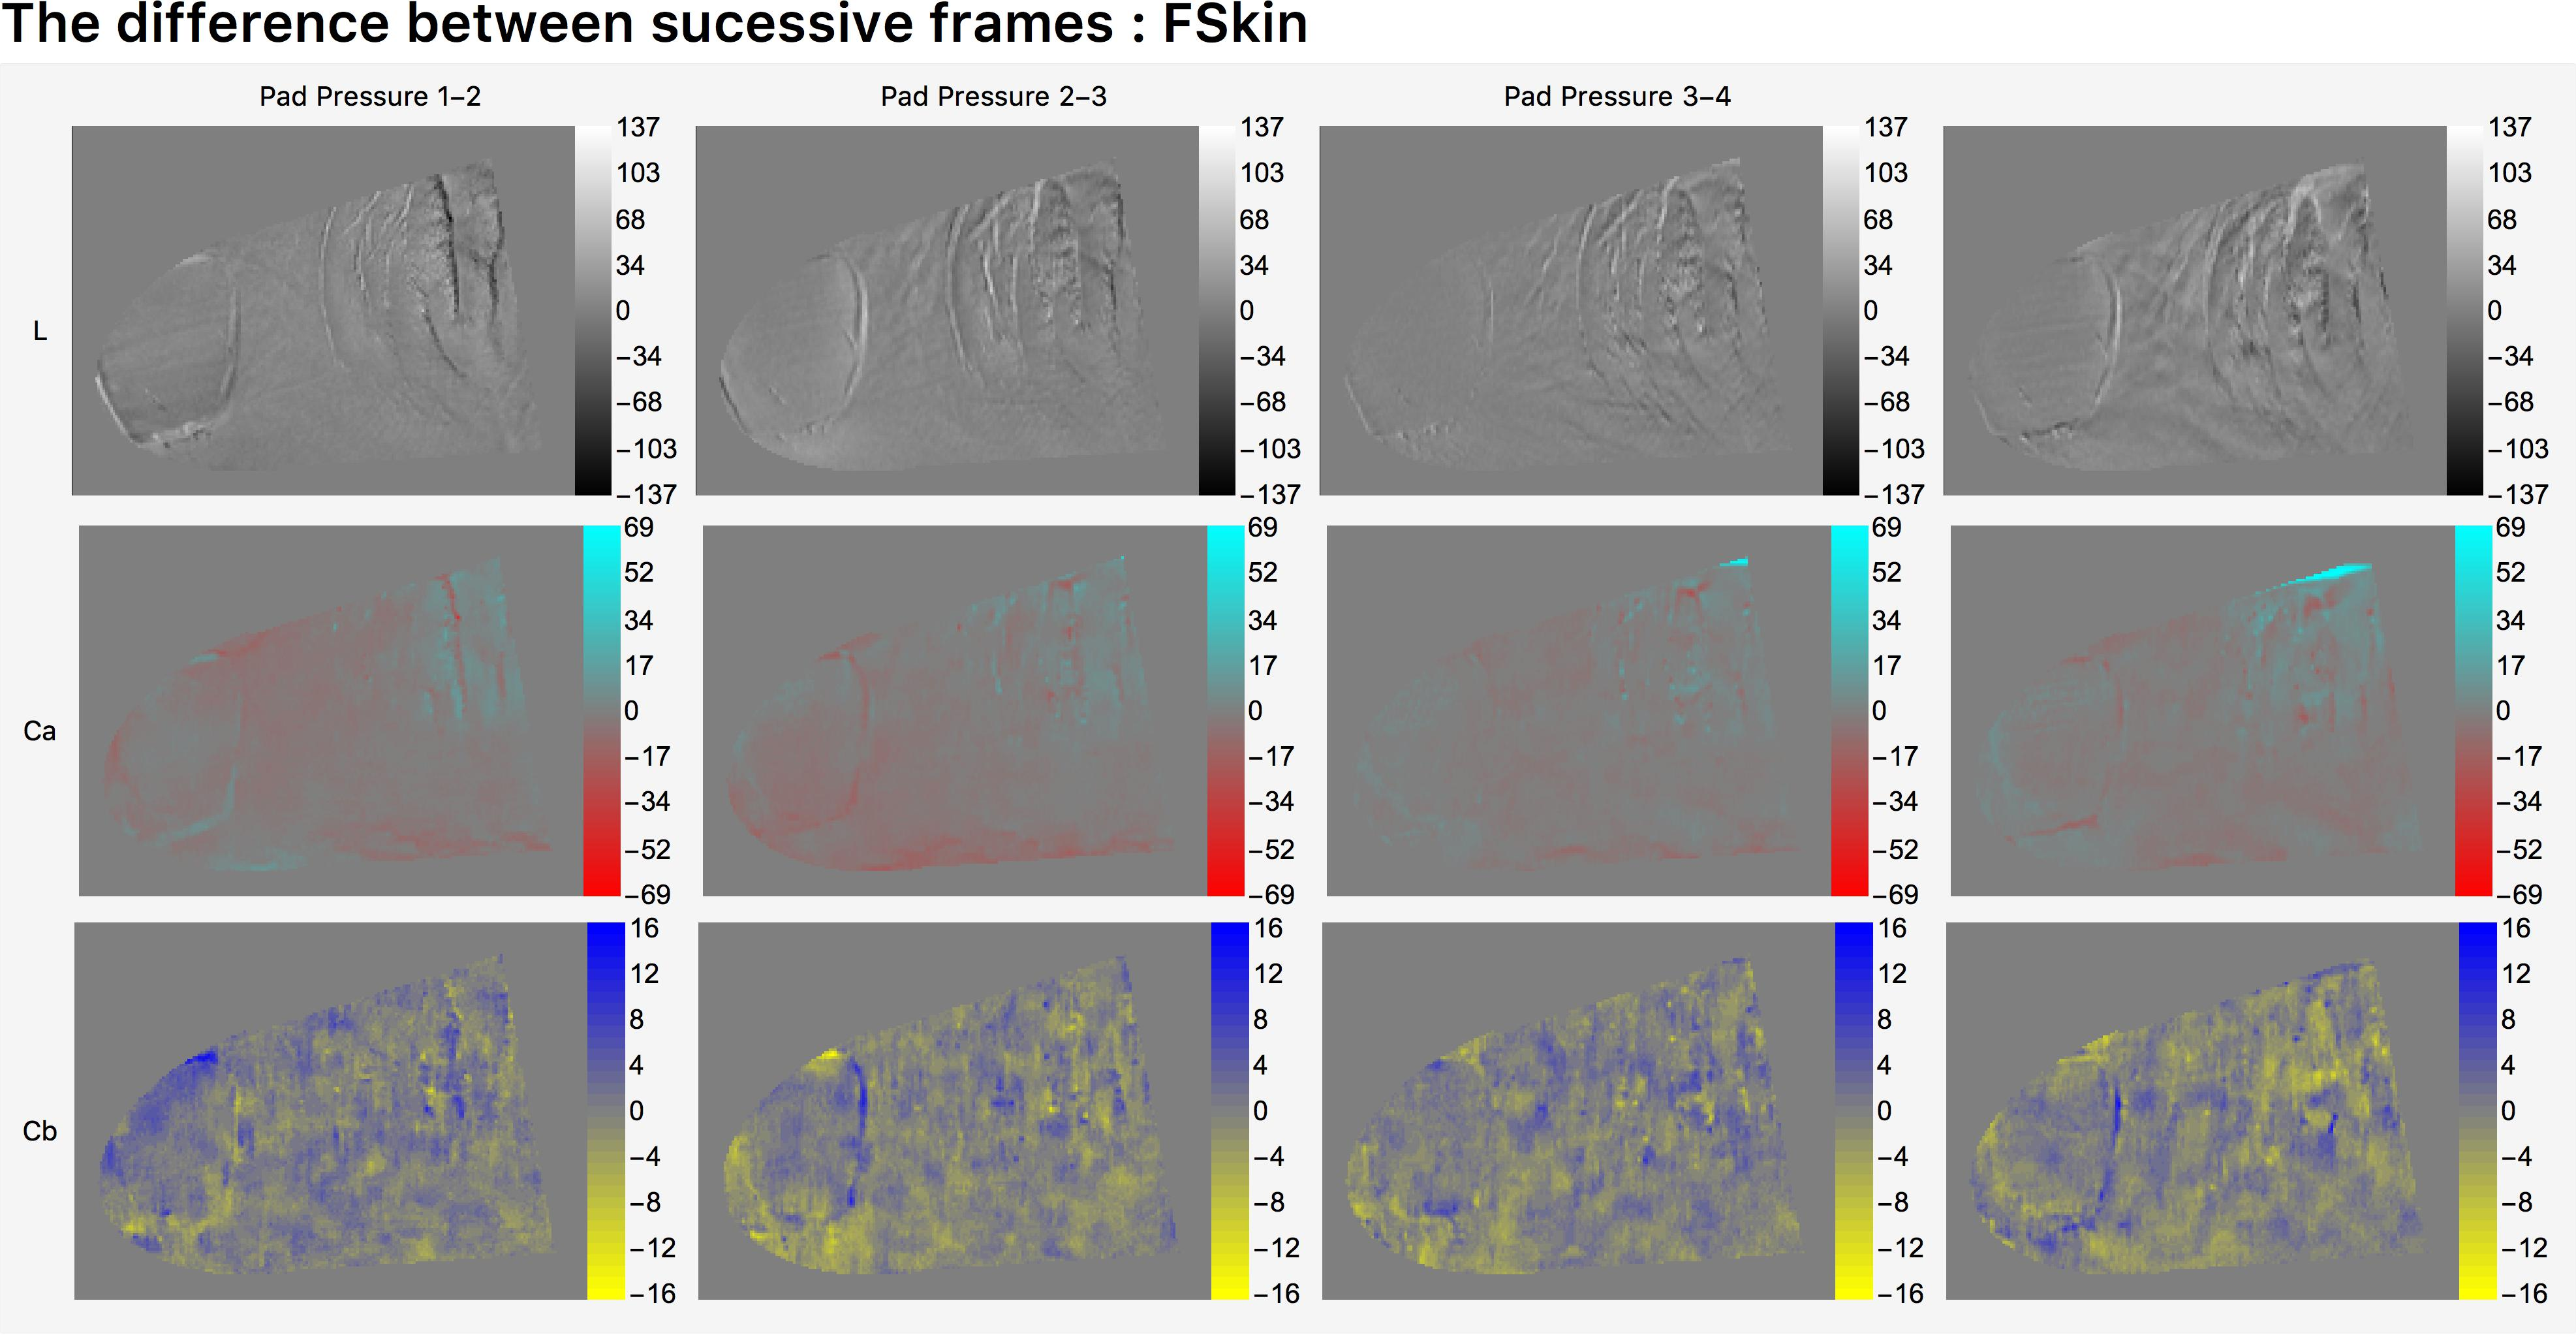
\includegraphics[width=0.660\textwidth]{Chapter4/Figs/Final_Fig_Difference_FSkin.jpg}
    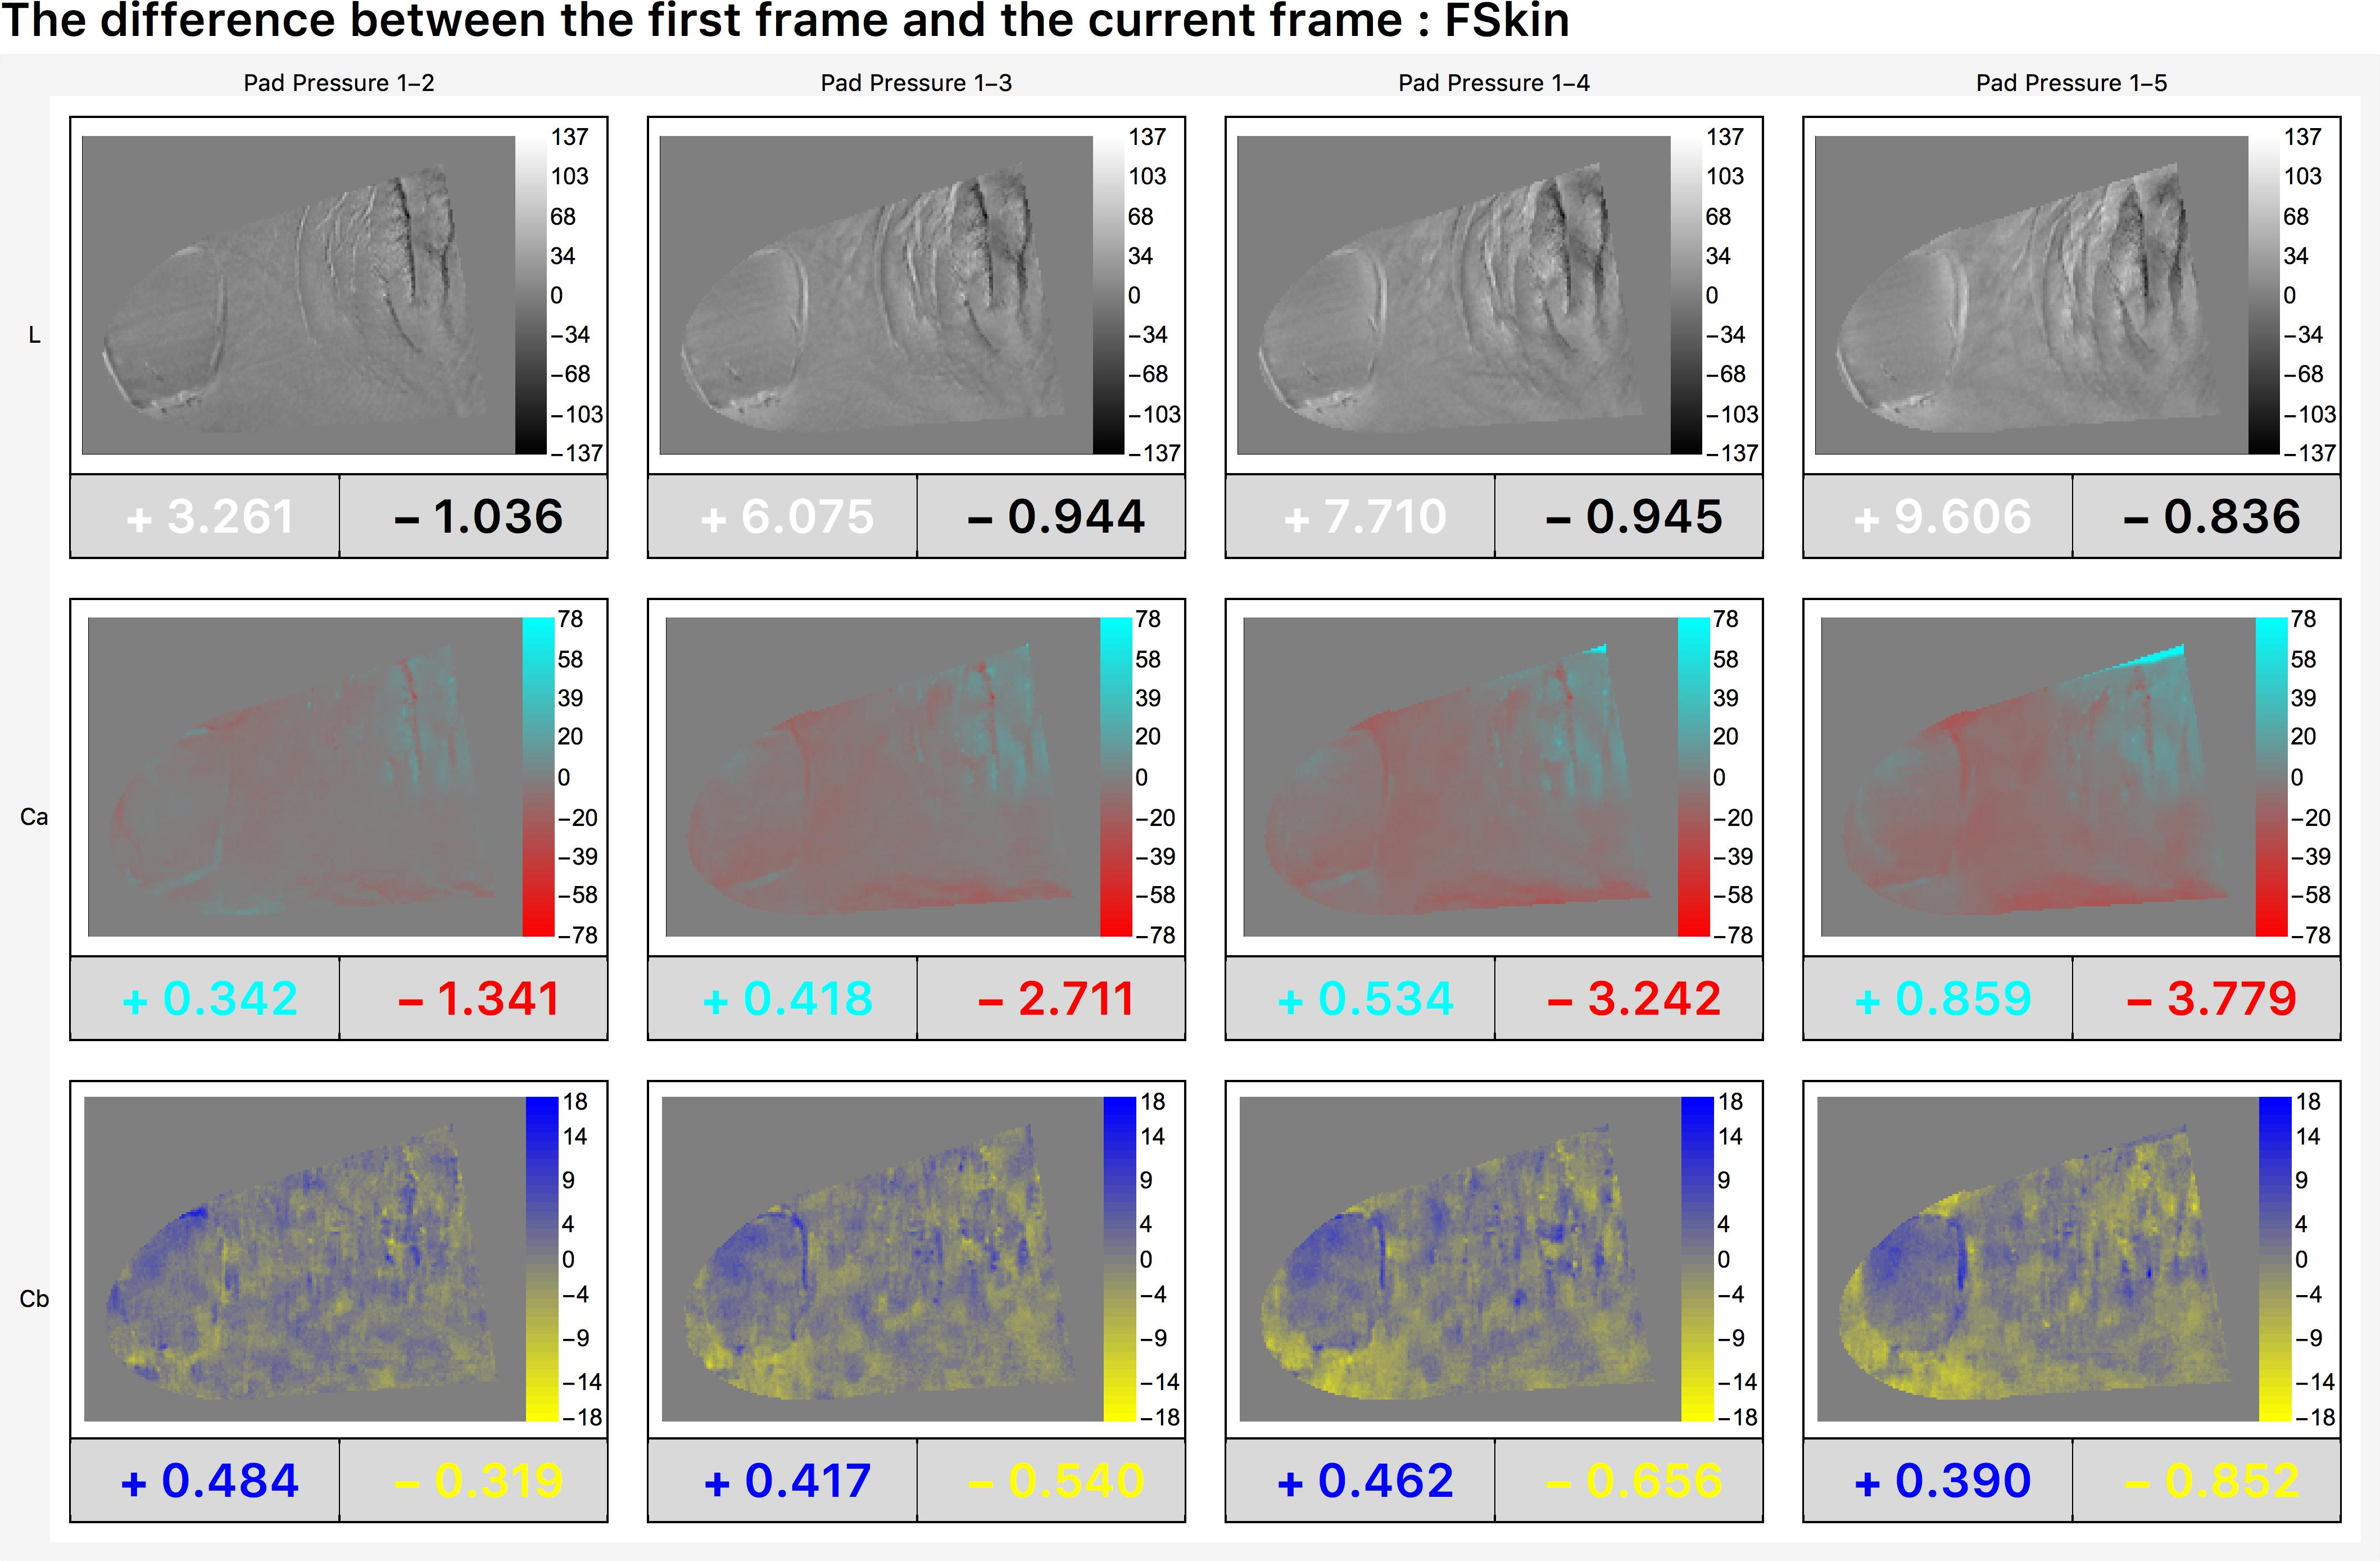
\includegraphics[width=0.660\textwidth]{Chapter4/Figs/Final_Fig_Total_Difference_FSkin.jpg}
    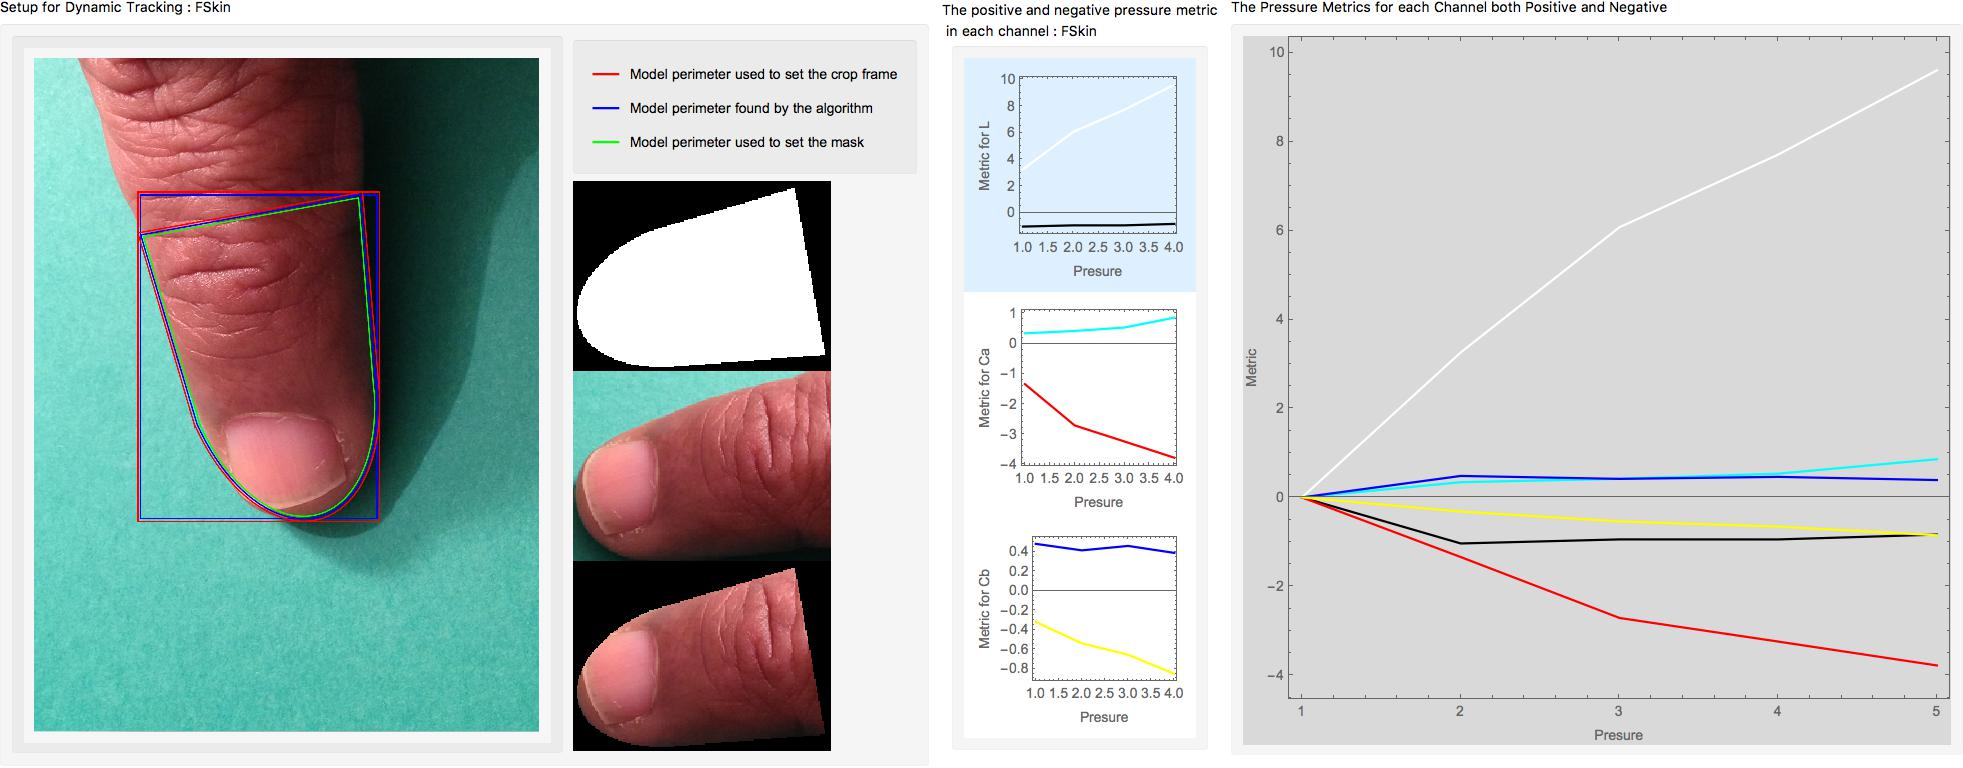
\includegraphics[width=0.820\textwidth]{Chapter4/Figs/Final_Fig_Misc_FSkin.jpg}
        \caption{The resulting sequence of images from the ICWaS algorithm followed by the differences. The metric is the result of summing the positive and negative changes separately and then dividing by the number of pixels. Finally, the initial image of the sequence is shown with the model outline, the slightly larger model used to set the crop frame and the slightly smaller model used for setting the mask.}\label{fig:ICWaSResultFSkin}
\end{figure}


\begin{figure}[h!]
  \centering
    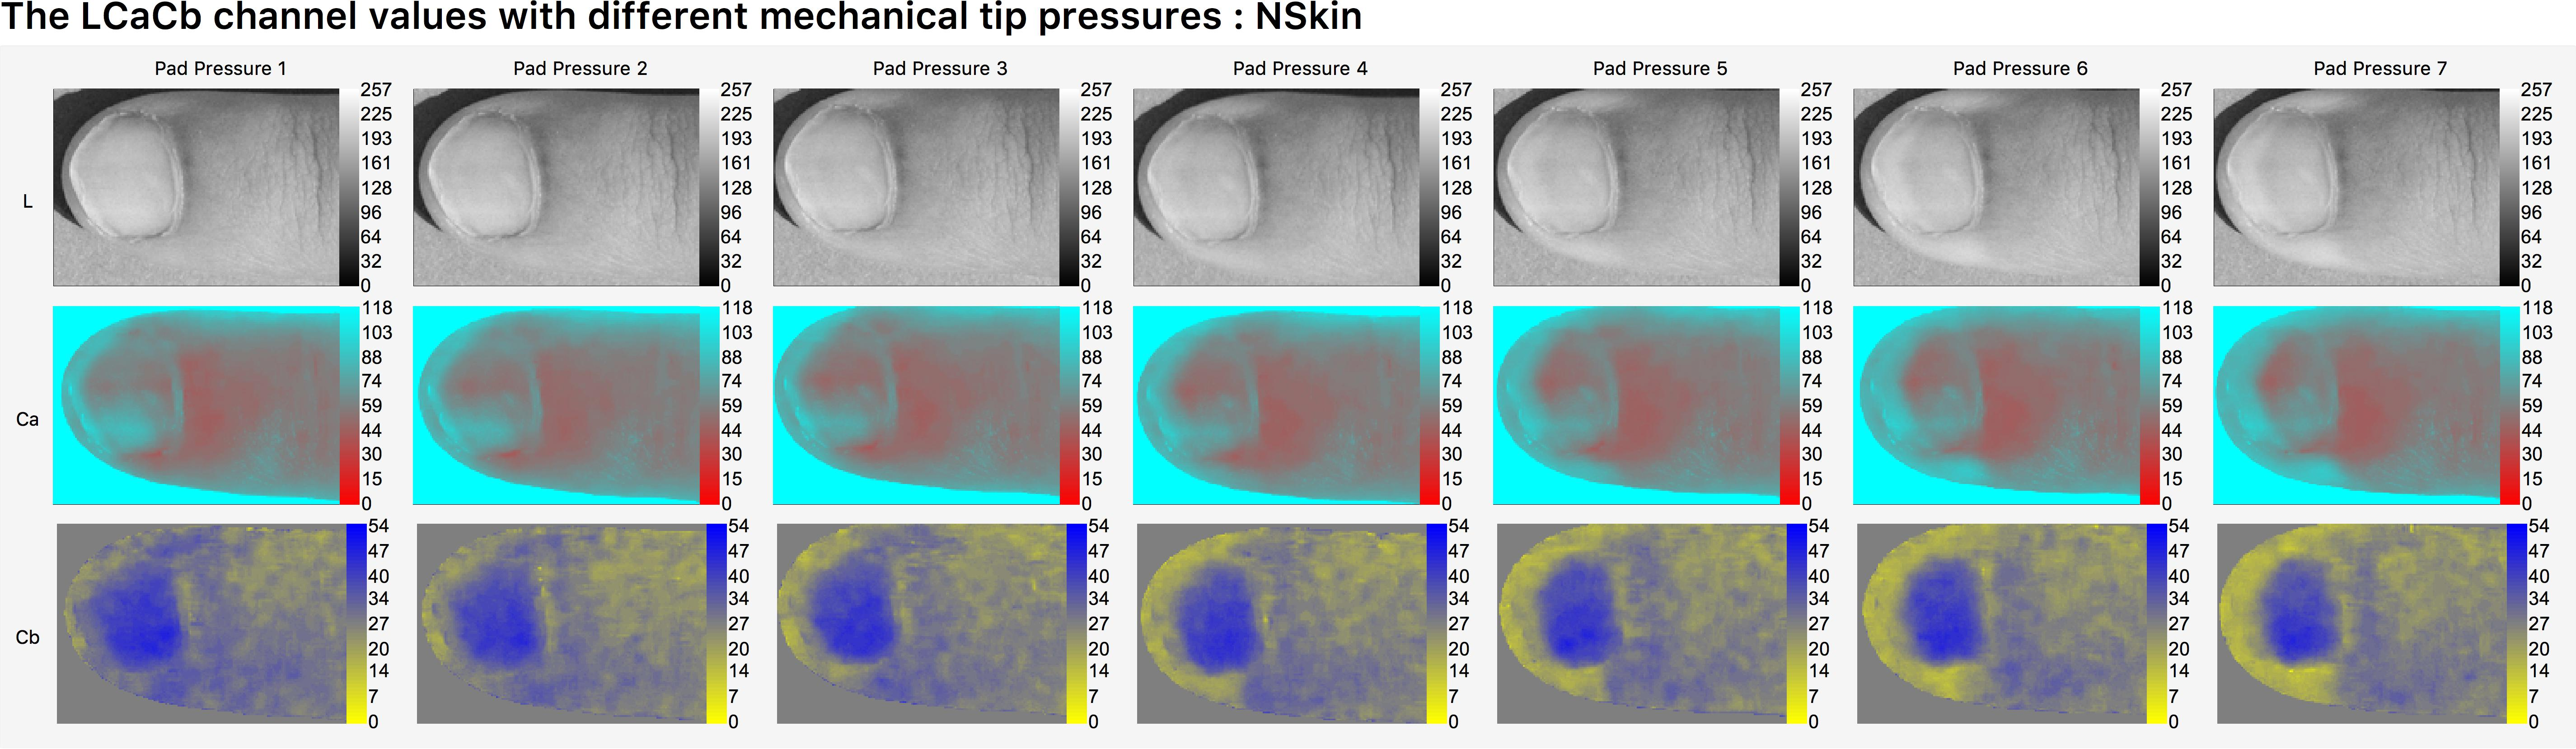
\includegraphics[width=1.00\textwidth]{Chapter4/Figs/Final_Fig_Channels_NSkin.jpg}
%    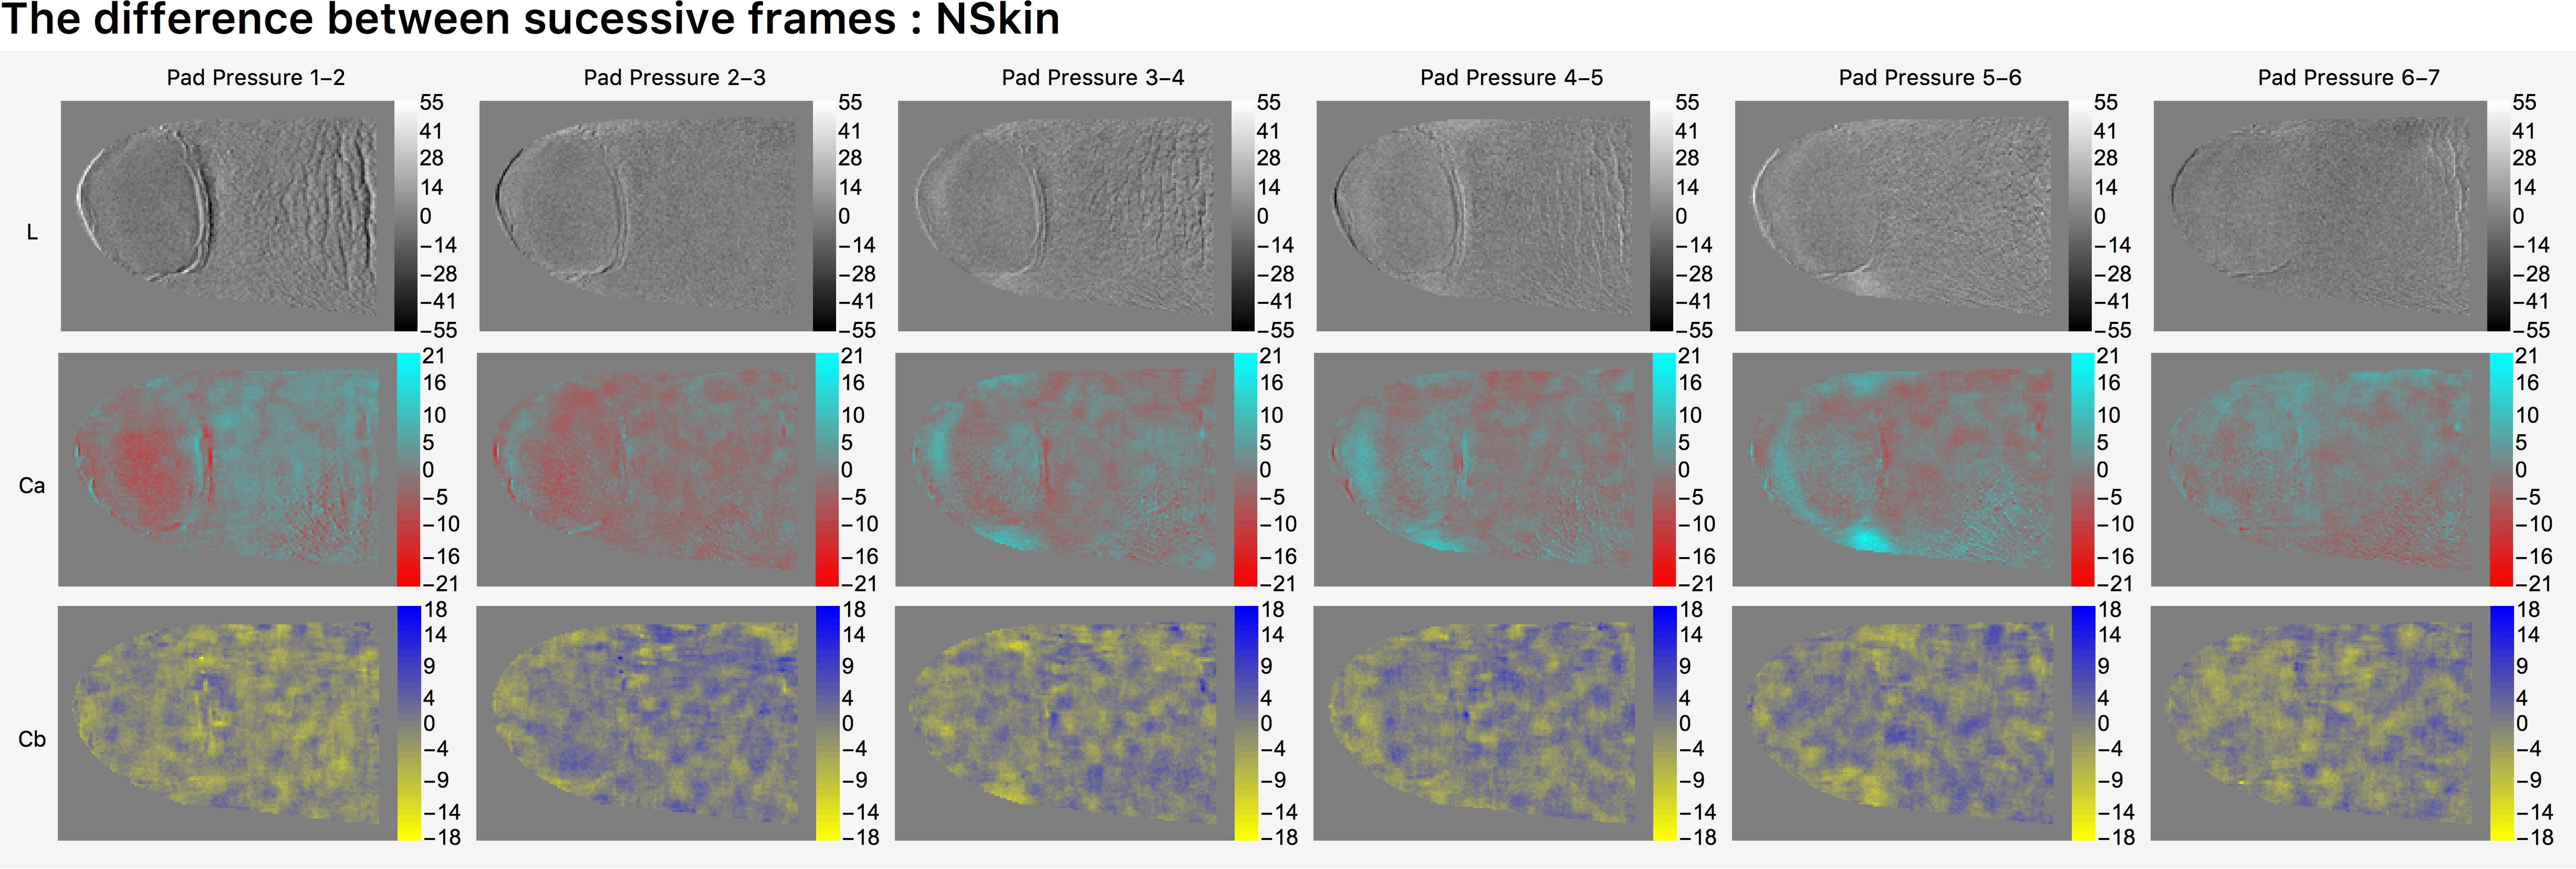
\includegraphics[width=0.86\textwidth]{Chapter4/Figs/Final_Fig_Difference_NSkin.jpg}
    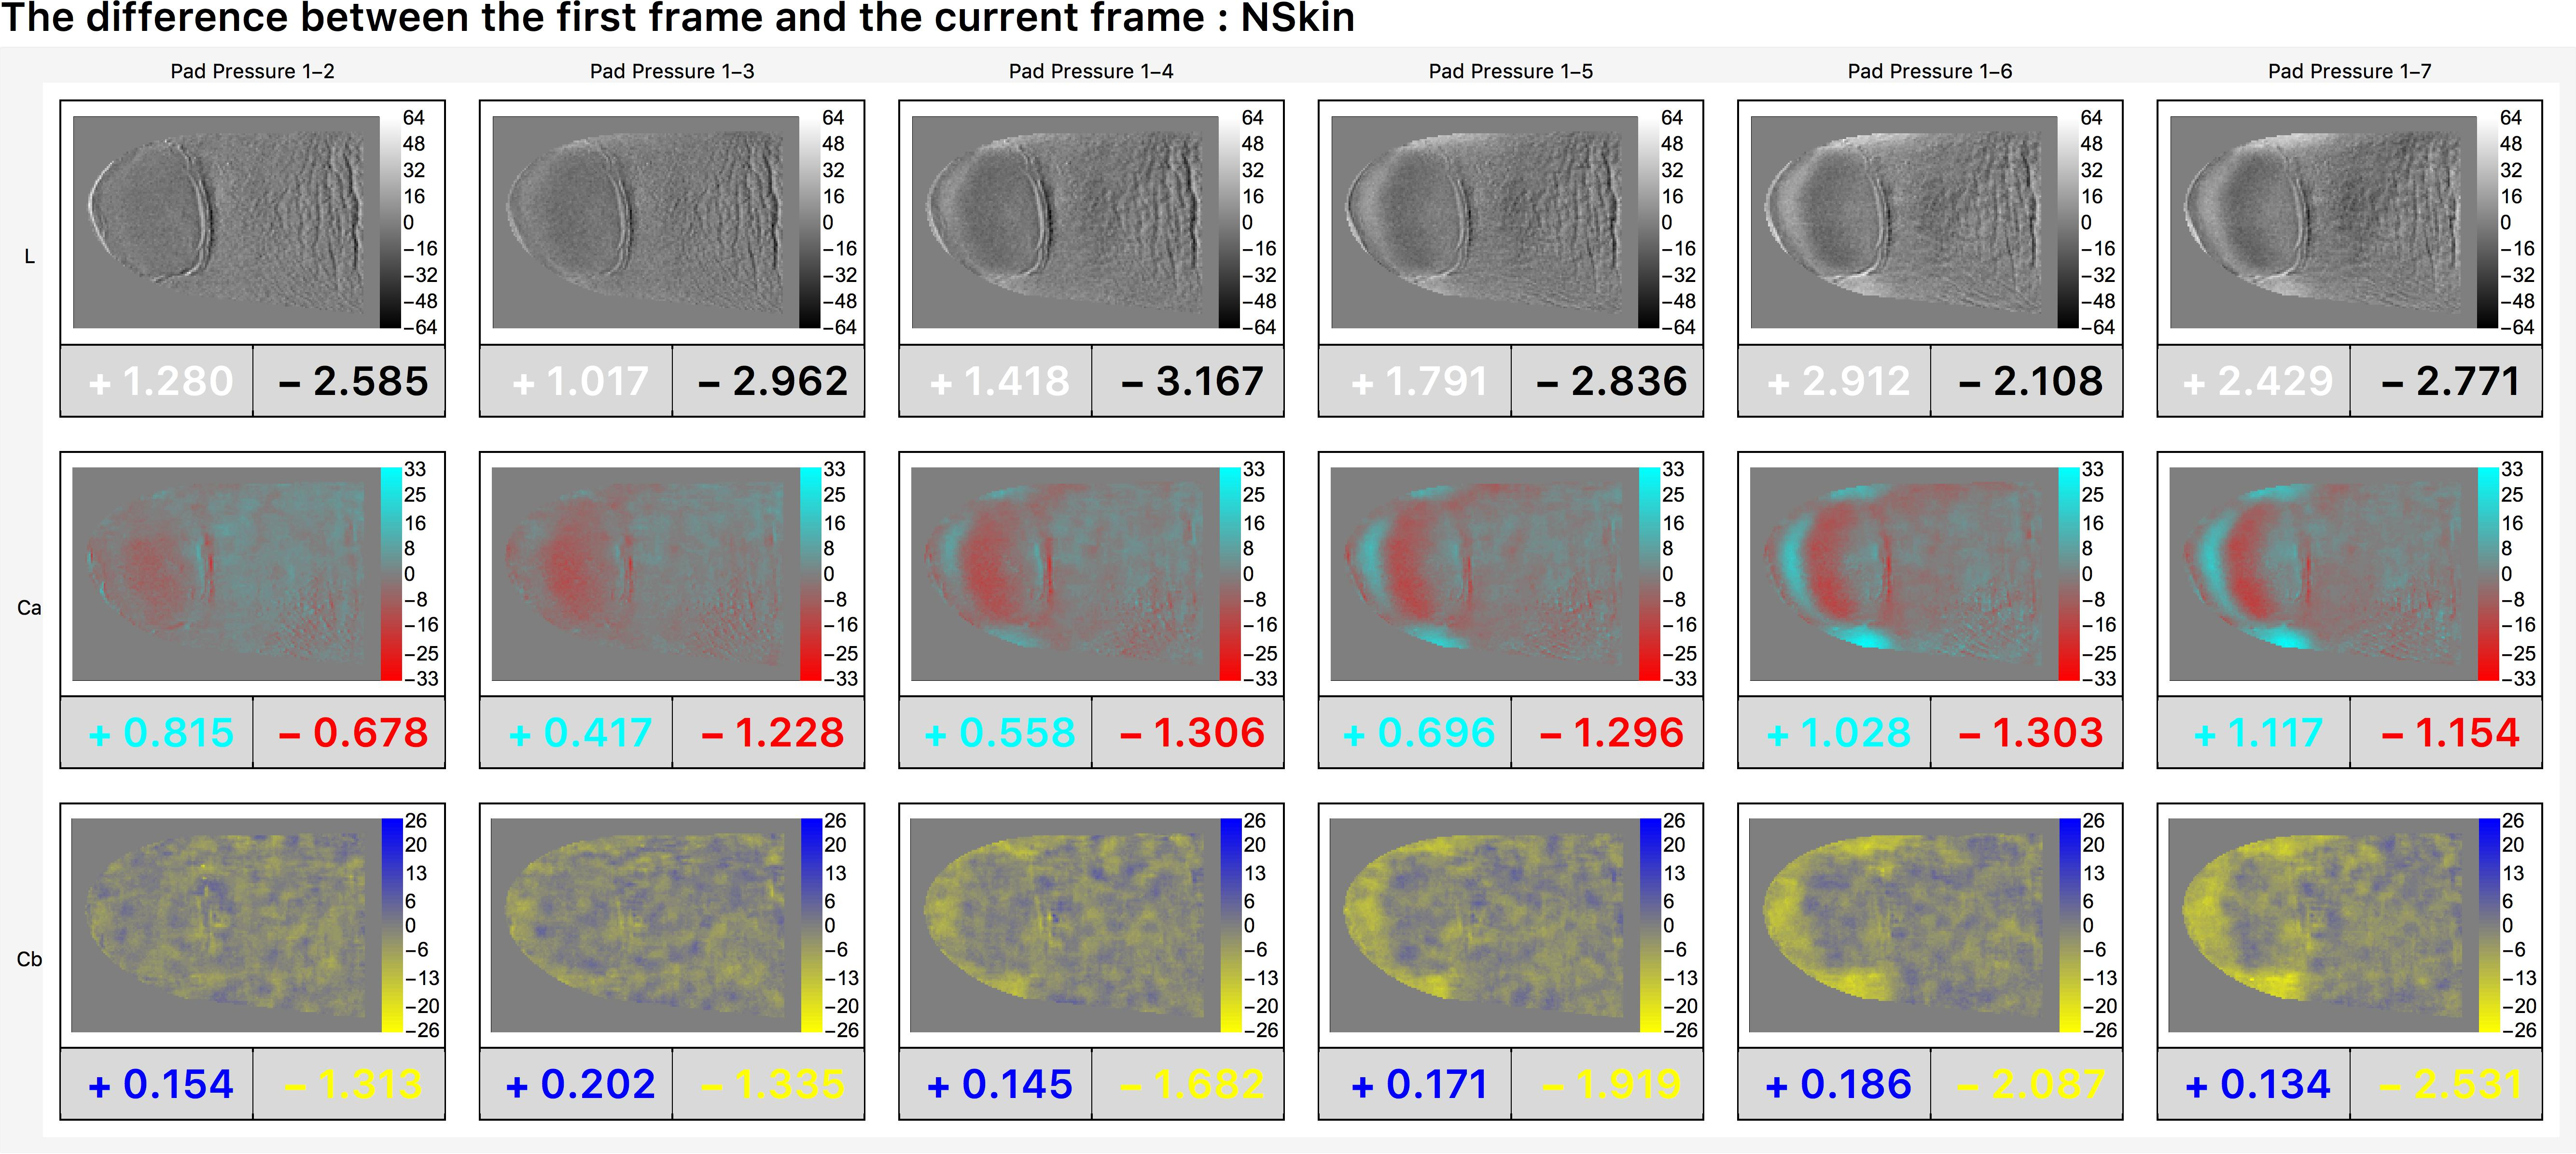
\includegraphics[width=0.86\textwidth]{Chapter4/Figs/Final_Fig_Total_Difference_NSkin.jpg}
    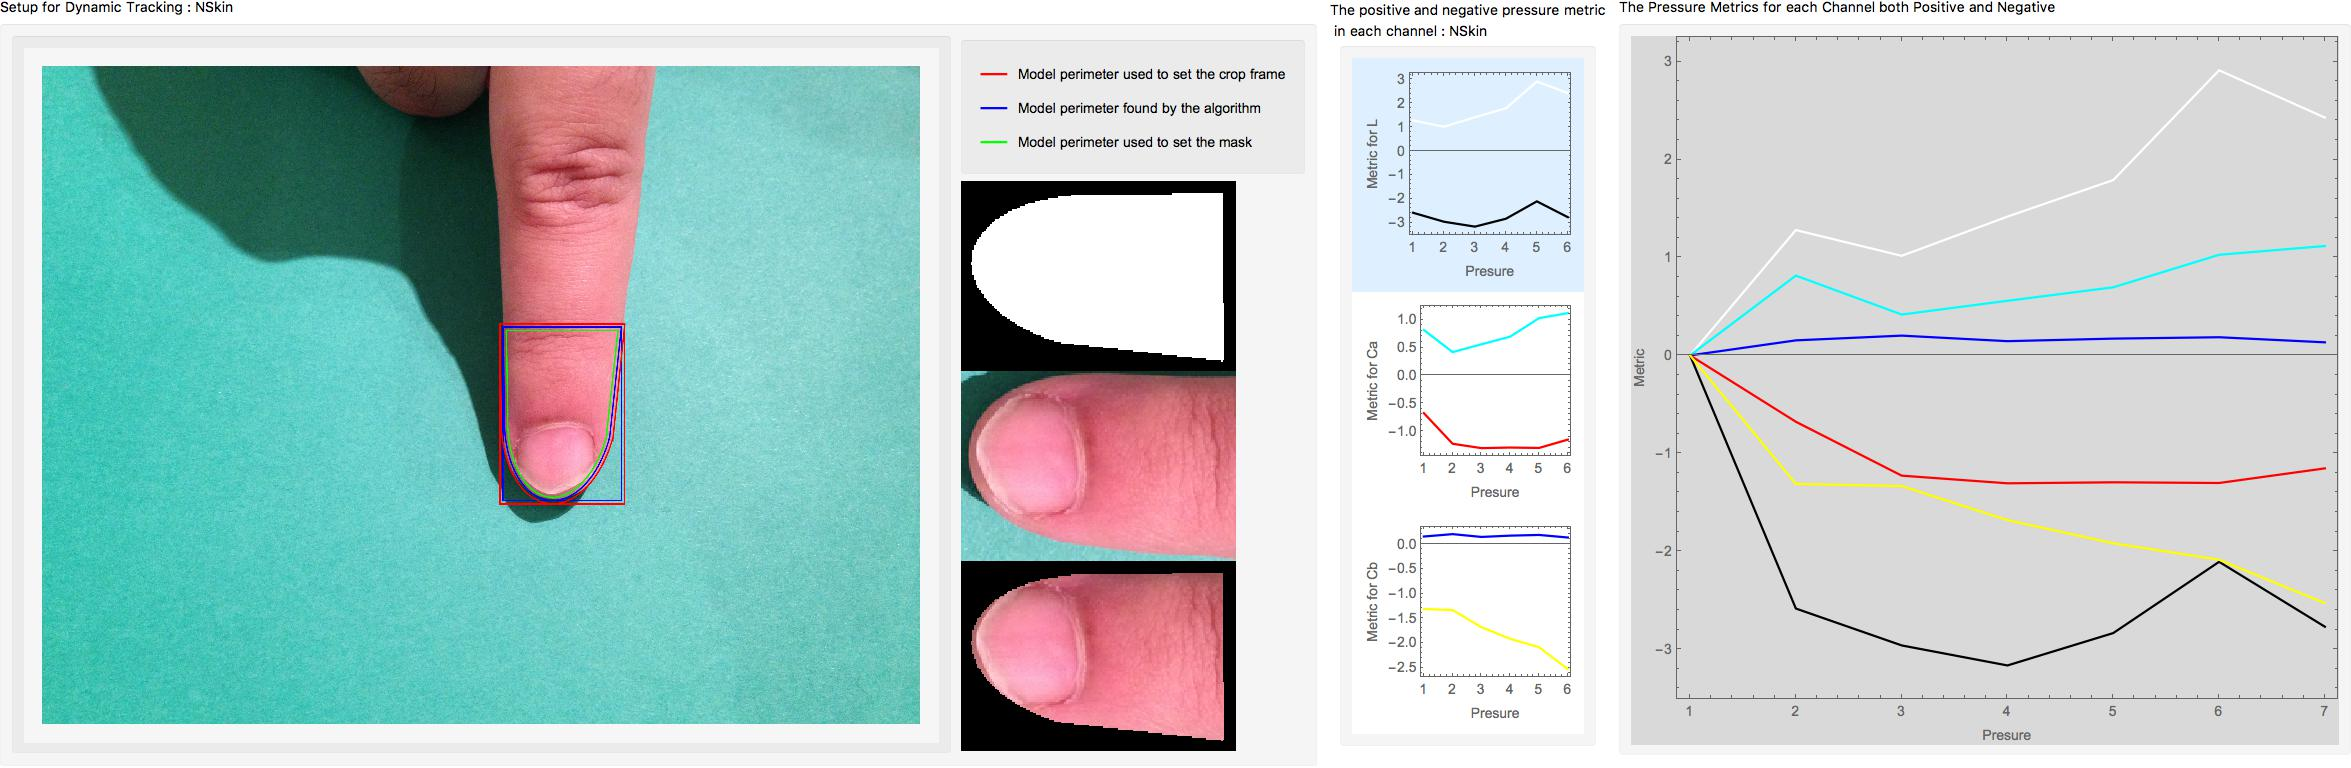
\includegraphics[width=1.00\textwidth]{Chapter4/Figs/Final_Fig_Misc_NSkin.jpg}
        \caption{The resulting sequence of images from the ICWaS algorithm followed by the differences. The metric is the result of summing the positive and negative changes separately and then dividing by the number of pixels. Finally, the initial image of the sequence is shown with the model outline, the slightly larger model used to set the crop frame and the slightly smaller model used for setting the mask.}\label{fig:ICWaSResultNSkin}
\end{figure}

We assume that the digit's movement will not take it outside of the bounding box set up in the initialization step (Section \ref{sec:ICWaSSetup}), so we capture the tip image from the video feed. The RGB tip image is converted to the skin color-space, then the grayscale channel image is used to align with the previous captured frame; if this is the first pass through the loop, this is the image captured in the initialization. The frame alignment metric is masked using the binary rastered model image generated in the initialization.

The image alignment pixel shift updates the change in the model position since the first frame. If the change in the model position since the first frame is greater than the ICWaS threshold, then the control passes back to the Smooth Motion routine. The current frame is aligned with the previous frame and the difference is found between the pixel values in the chromatic channels; this is the blood flow (Figures  \ref{fig:ICWaSResultJSkin}, \ref{fig:ICWaSResultFSkin} \& \ref{fig:ICWaSResultNSkin}). These steps are repeated until the change in the model position since the first frame causes the routine to transfer control back to the Smooth Motion routine.

\clearpage

\subsubsection{Blood Flow Metric}\label{sec:BloodFlowMetric}

\begin{figure}[tbph]
\centering
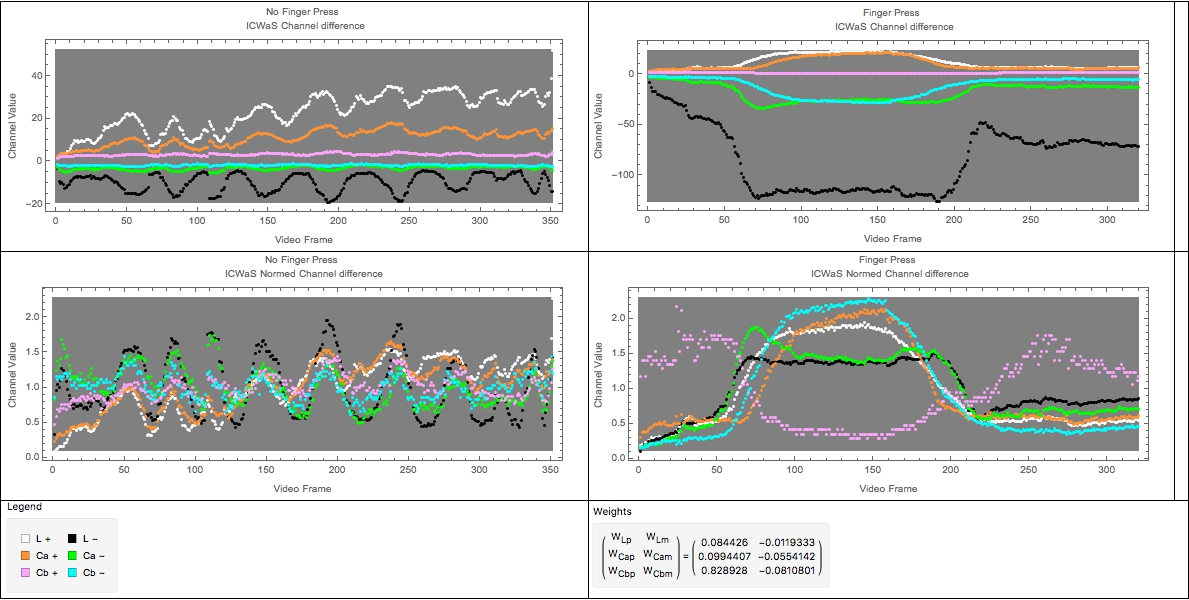
\includegraphics[width=0.95\linewidth]{Chapter4/Figs/sixChannelsWeightsGrfx}
\caption[Normalized the 6-channel metrics.]{The normalized 6-channel metrics, revealing the shape of the distributions and facilitating numerical techniques.}
\label{fig:sixchannelsweightsgrfx}
\end{figure}
\begin{figure}[tbph]
\centering
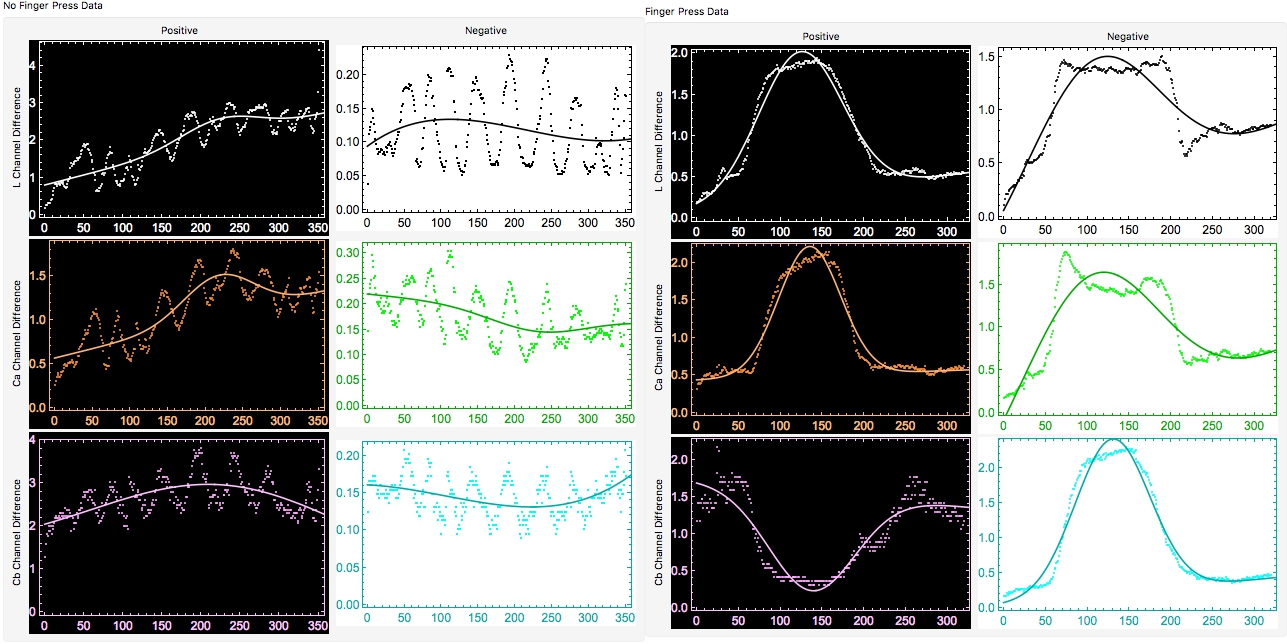
\includegraphics[width=0.95\linewidth]{Chapter4/Figs/sixChannelFitGrfx}
\caption{A functional fit to the 6-channel metrics for both the 'Press' and 'No-Press' data. The fit uses a combination of a Gaussian and a straight line.}
\label{fig:sixchannelfitgrfx}
\end{figure}
\begin{figure}[tbph]
\centering
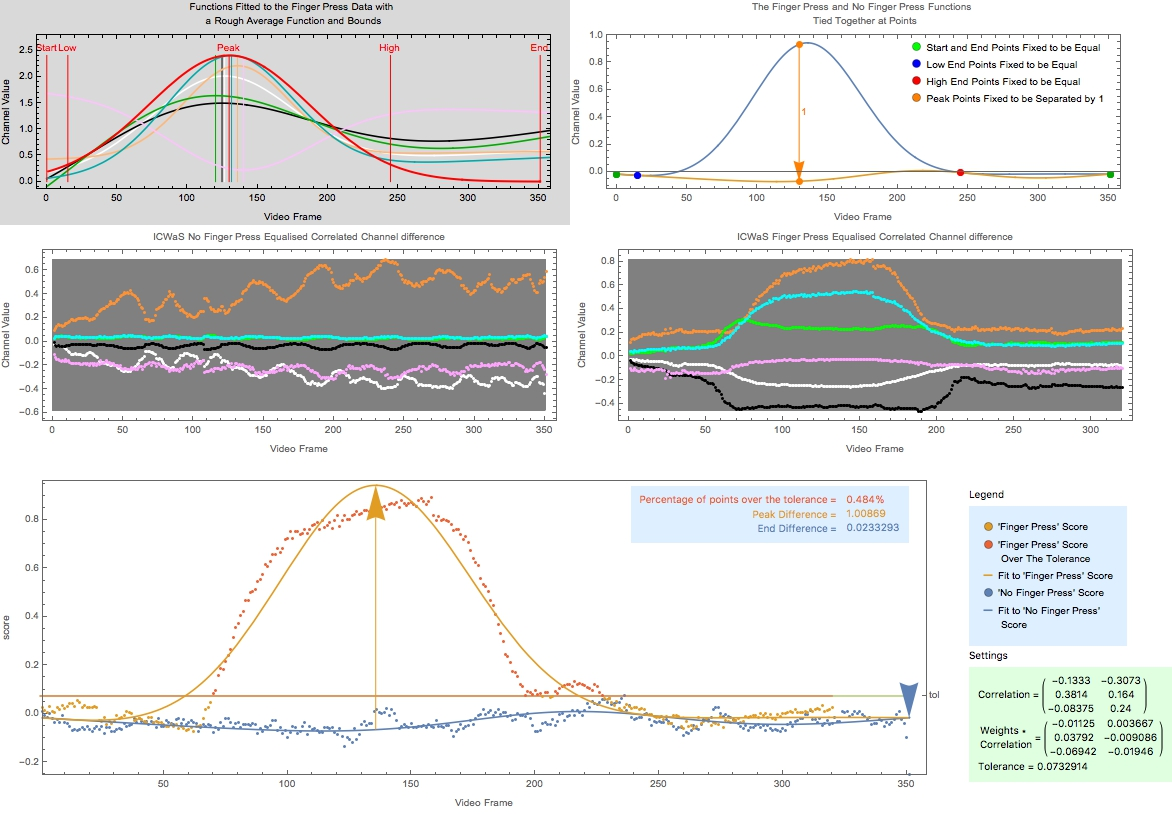
\includegraphics[width=0.95\linewidth]{Chapter4/Figs/anyliticCorrelationGrfx}
\caption[The Analytic Correlation.]{The Analytic Correlation. Fixing the points for the linear combination, as seen in top right diagram, an analytic solution is found for the correlation matrix.}
\label{fig:anyliticcorrelationgrfx}
\end{figure}
\begin{figure}[tbph]
\centering
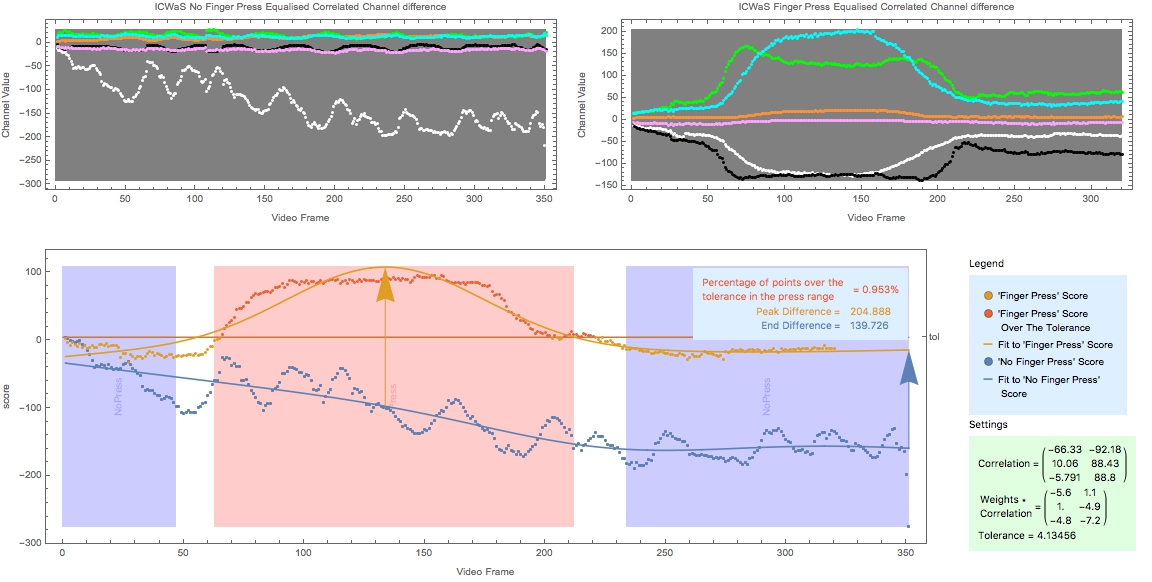
\includegraphics[width=0.95\linewidth]{Chapter4/Figs/numericCorrelationGrfx}
\caption{The numerically-found correlation matrix.}
\label{fig:numericcorrelationgrfx}
\end{figure}


\newcommand{\mL}{L^-}
\newcommand{\pL}{L^+}
\newcommand{\mCa}{Ca^-}
\newcommand{\pCa}{Ca^+}
\newcommand{\mCb}{Cb^-}
\newcommand{\pCb}{Cb^+}

\newcommand{\CmL}{C_{\mL}}
\newcommand{\CpL}{C_{\pL}}
\newcommand{\CmCa}{C_{\mCa}}
\newcommand{\CpCa}{C_{\pCa}}
\newcommand{\CmCb}{C_{\mCb}}
\newcommand{\CpCb}{C_{\pCb}}
We have a 6-channel metric from the ICWaS method which we wish to use to detect the presence of mechanical stress in the tip, i.e. the finger tip pressing on the surface. The simplest solution is to form a linear combination of the 6-channel metric and to set a threshold above which the finger tip is considered to be pressing on the surface. 

The metric needs to be able to distinguish between the finger sliding slowly across the surface and the finger pressing on the surface. Two ICWaS runs are compared in Figure  \ref{fig:sixchannelsweightsgrfx}, one with the finger sliding slowly across the surface ('No-Press' data), and the other with the finger pressing on the surface then releasing pressure ('Press' data). 

First, the 6-channel metrics are normalized to reveal the shape of the distributions and to facilitate numerical techniques (Figure \ref{fig:sixchannelsweightsgrfx}). Then we fit a function, which is a combination of a straight line with a Gaussian, to the two sets of data, as seen in Figure \ref{fig:sixchannelfitgrfx}. 
\begin{equation}
f^{set}_{channel} (x) = A e^{-\frac{0.5 (x-\mu )^2}{\sigma ^2}}+m x +c
\end{equation}
The 6 Press data functions clearly exhibit a common peak  and a similar variance, as illustrated in Figure \ref{fig:anyliticcorrelationgrfx}. This allows the Press data to be divided into regions where we want the combined metric to register minimally and maximally. It is also desirable for the combined metric to be flat when no pressure is being applied. These considerations allow a set of equations to be defined:


\newlength{\savedbelowdisplayskip}
\newlength{\savedabovedisplayskip}
\newlength{\savedbelowdisplayshortskip}
\newlength{\savedabovedisplayshortskip}

\setlength{\savedbelowdisplayskip}{\belowdisplayskip} \setlength{\savedbelowdisplayshortskip}{\belowdisplayshortskip}
\setlength{\savedabovedisplayskip}{\abovedisplayskip} \setlength{\savedabovedisplayshortskip}{\abovedisplayshortskip}

\setlength{\belowdisplayskip}{0pt} \setlength{\belowdisplayshortskip}{0pt}
\setlength{\abovedisplayskip}{0pt} \setlength{\abovedisplayshortskip}{0pt}


\begin{multline*}
F^{np}(x) =    \CmCa F^{np}_{\mCa}(x) + \CpCa F^{np}_{\pCa}(x) +   \\
  \CmCb F^{np}_{\mCb}(x) + \CpCb F^{np}_{\pCb}(x) +   \\ 
  \CmL    F^{np}_{  \mL}(x) + \CpL   F^{np}_{   \pL}(x)   
\end{multline*} 
\begin{multline}
F^{p}(x) =  
 \CmCa F^{p}_{\mCa}(x) + \CpCa F^{p}_{\pCa}(x) +  \\
  \CmCb F^{p}_{\mCb}(x) + \CpCb F^{p}_{\pCb}(x) + \\ 
   \CmL    F^{p}_{  \mL}(x) + \CpL   F^{p}_{   \pL}(x) 
\end{multline}\label{eqn:FnpFp}
\begin{align}
F^{np}(x_{start}) & = F^{p}(x_{start}) = F^{np}(x_{end}) = F^{p}(x_{end}) \nonumber  \\
F^{np}(x_{low}) & = F^{p}(x_{low})  \nonumber  \\
F^{np}(x_{high}) & = F^{p}(x_{high})  \label{eqn:AnanyticSolutionConditions}
\end{align}


\setlength{\belowdisplayskip}{\savedbelowdisplayskip} \setlength{\belowdisplayshortskip}{\savedbelowdisplayshortskip}
\setlength{\abovedisplayskip}{\savedabovedisplayskip} \setlength{\abovedisplayshortskip}{\savedabovedisplayshortskip}

These conditions (Equation \ref{eqn:AnanyticSolutionConditions}) can be solved for finding the 6 linear coefficients (Equation \ref{eqn:FnpFp}). The results can be seen in Figure \ref{fig:anyliticcorrelationgrfx}.

For completeness, a numerical technique to find the 6 linear coefficients was also attempted. The success was scored by checking the 'correct' classification of the data as Press or No-Press. The results can be seen in Figure \ref{fig:numericcorrelationgrfx}. 

The two different methods were run using data from different individuals and different digits. 



\subsection{Dynamic State Transitions}\label{sec:DynamicStateTransitions}
For each of the three states, we need to define a metric which characterizes the motion detected. Using these metrics, we need to define four tolerances for the state transitions.

The metric for the rapid motion detection is the average pixel value of the eroded difference image (Section \ref{sec:DynamicTracking}), so if two consecutive images are the same, then the metric is 0. And if every pixel has changed by its maximum amount (e.g. every pixel black/white), then the metric is 255. The only question remaining is what sort of values should we expect for rapid finger movement. We can roughly estimate that a finger occupies about 10\% of the frame; given that the background is illuminated by the same amount, we can expect pixel differences around 20\%. Thus, although the range of the metric is actually 0-255, we actually expect the tolerance to be quite low.

\begin{figure}[tbph]
\centering
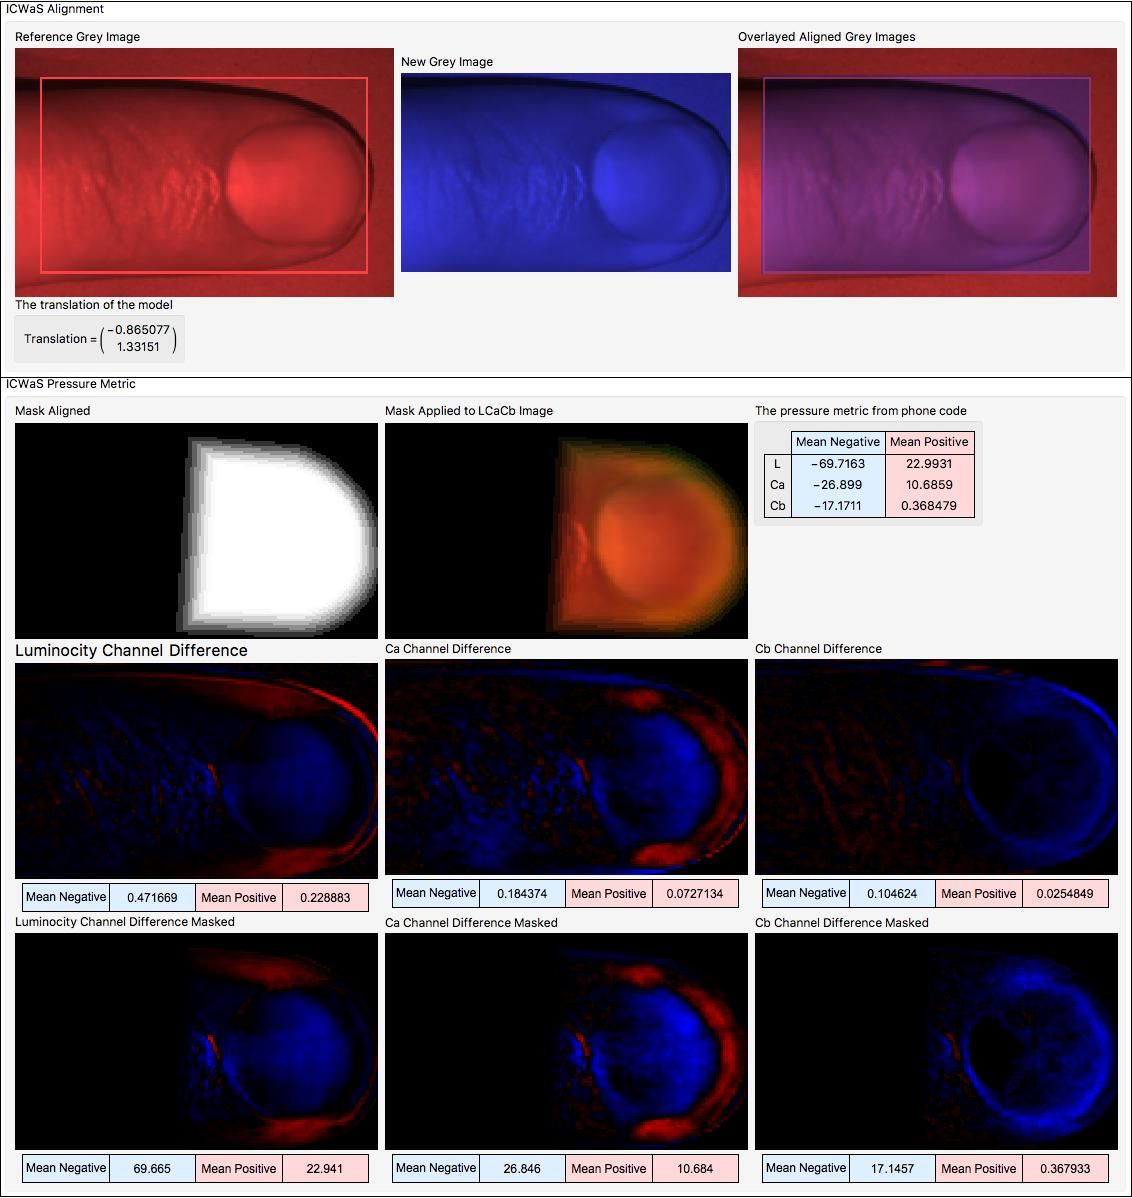
\includegraphics[width=0.95\linewidth]{Chapter4/Figs/ICWaSAlignment&Metric}
\caption{ICWaS alignment and Metric}
\label{fig:icwasalignmentmetric}
\end{figure}

The metric for the smooth motion detection is the pixel distance moved by the model divided by the distal width, as seen in Section \ref{sec:SmoothMotionTracking}. Significant values for this metric are 0 if the model hasn't had to move; 1 if the model is moved by a finger width; and it is assigned a negative value when the finger is not detected, moved out of frame, or if an insufficient amount of the digit remains in the frame. So, for negative values, the model isn't updated.

The ICWaS detection method returns the distance that the bounding box for the fingertip has had to move to align the image with the previous frame (Section \ref{sec:ICWaS}). OpenCV's alignment routine requires the images to be well-aligned in order to function properly, so before attempting alignment, the code initially checks for large movements and does not perform the alignment if such movement is detected, avoiding long iterations of OpenCV's routine which would ultimately result in an error. However, in order to make this robust, the routine also catches any error from the alignment routine. Both of these result in an negative value being returned.

\begin{figure}[tbph]
\centering
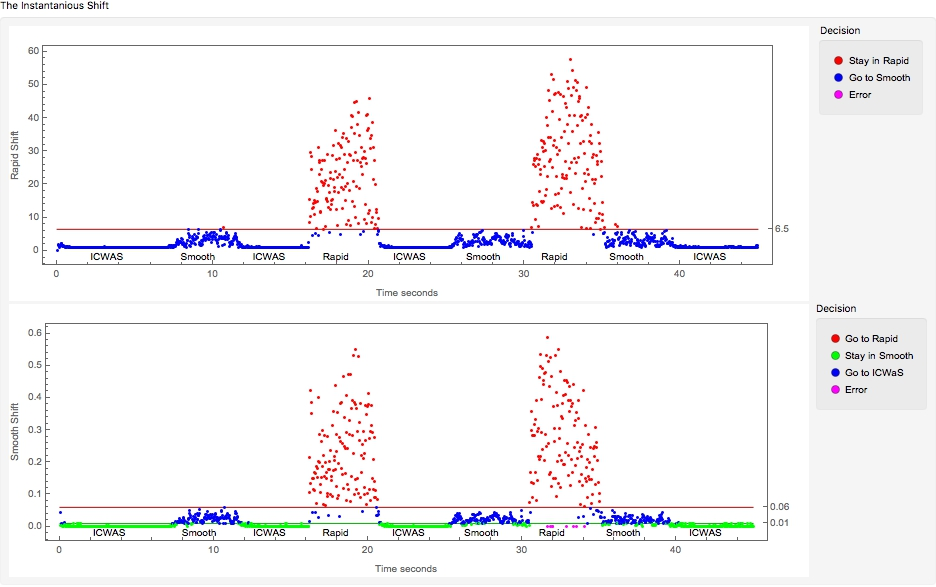
\includegraphics[width=0.95\linewidth]{Chapter4/Figs/instantaniousShiftGrfx}
\caption{The rapid and smooth dynamic tracking metrics.}
\label{fig:instantaniousshiftgrfx}
\end{figure}

In order to set reasonable values for the tolerances, a version of the code was written which, regardless of the state, performed both the rapid and smooth tracking routines. Using timed intervals, the code was run with the user performing motions which should be classified as a 'rapid movement, 'smooth movement' and 'ICWaS movement'. The results can be seen in Figure \ref{fig:instantaniousshiftgrfx}.

\begin{figure}[tbph]
\centering
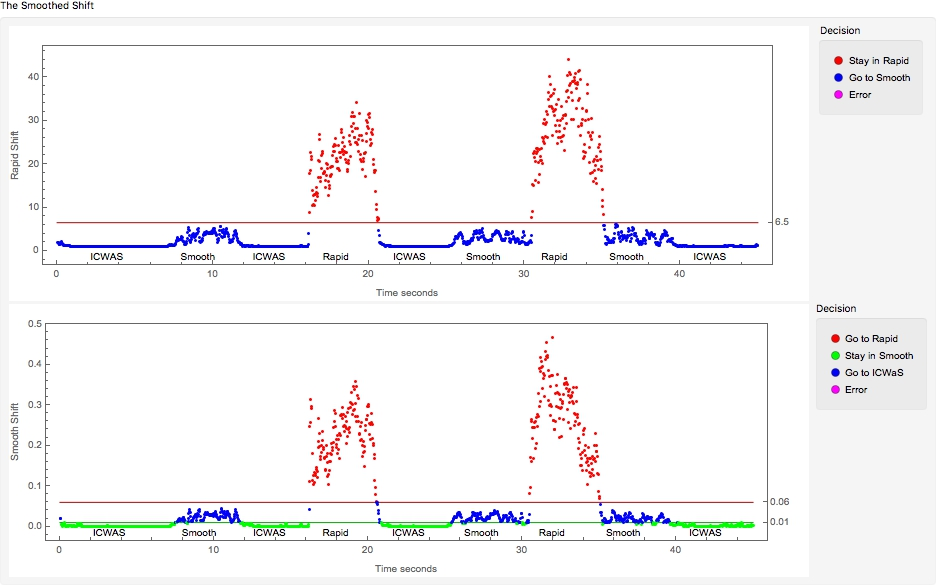
\includegraphics[width=0.95\linewidth]{Chapter4/Figs/smoothedShiftGrfx}
\caption{The rapid and smooth dynamic tracking metrics with values smoothed by averaging with previous values.}
\label{fig:smoothedshiftgrfx}
\end{figure}

From this figure, you can see the metrics are fairly noisy; we want to avoid triggering a state transition on the basis of a single video frame. This problem is effectively solved in the code simply by taking the average of the current metric with the previous value, thus smoothing out the noise and stabilizing the state transitions, as illustrated by Figure \ref{fig:smoothedshiftgrfx}.

\section{Putting it All Together}\label{sec:PuttingItAllTogether}
So far, we have said little about the app itself; the app associated with this project is designed to demonstrate how the fast color-space transform developed in Chapter 2 can be used in conjunction with the simple shape detection routines developed in this chapter to create a simple fingertip mechanical-stress detector using an iPhone.

Quite later on in development, an iOS update was released which allows in-code control of camera properties the algorithm which optimises these settings for the app is described in Appendix \ref{sec:iPhoneCameraSetup}.

It is considered good practice when developing an iPhone app to split the code into three parts: the model, which handles all the computation; the view, which handles display and interprets user gestures; and the controller, which is the intermediary. Each can be considered to be running in its own thread. The recommended division of the control assigns each step in the program as indicated in Figure \ref{fig:FingerpressUI}. 

\begin{figure}[h!]
  \centering
    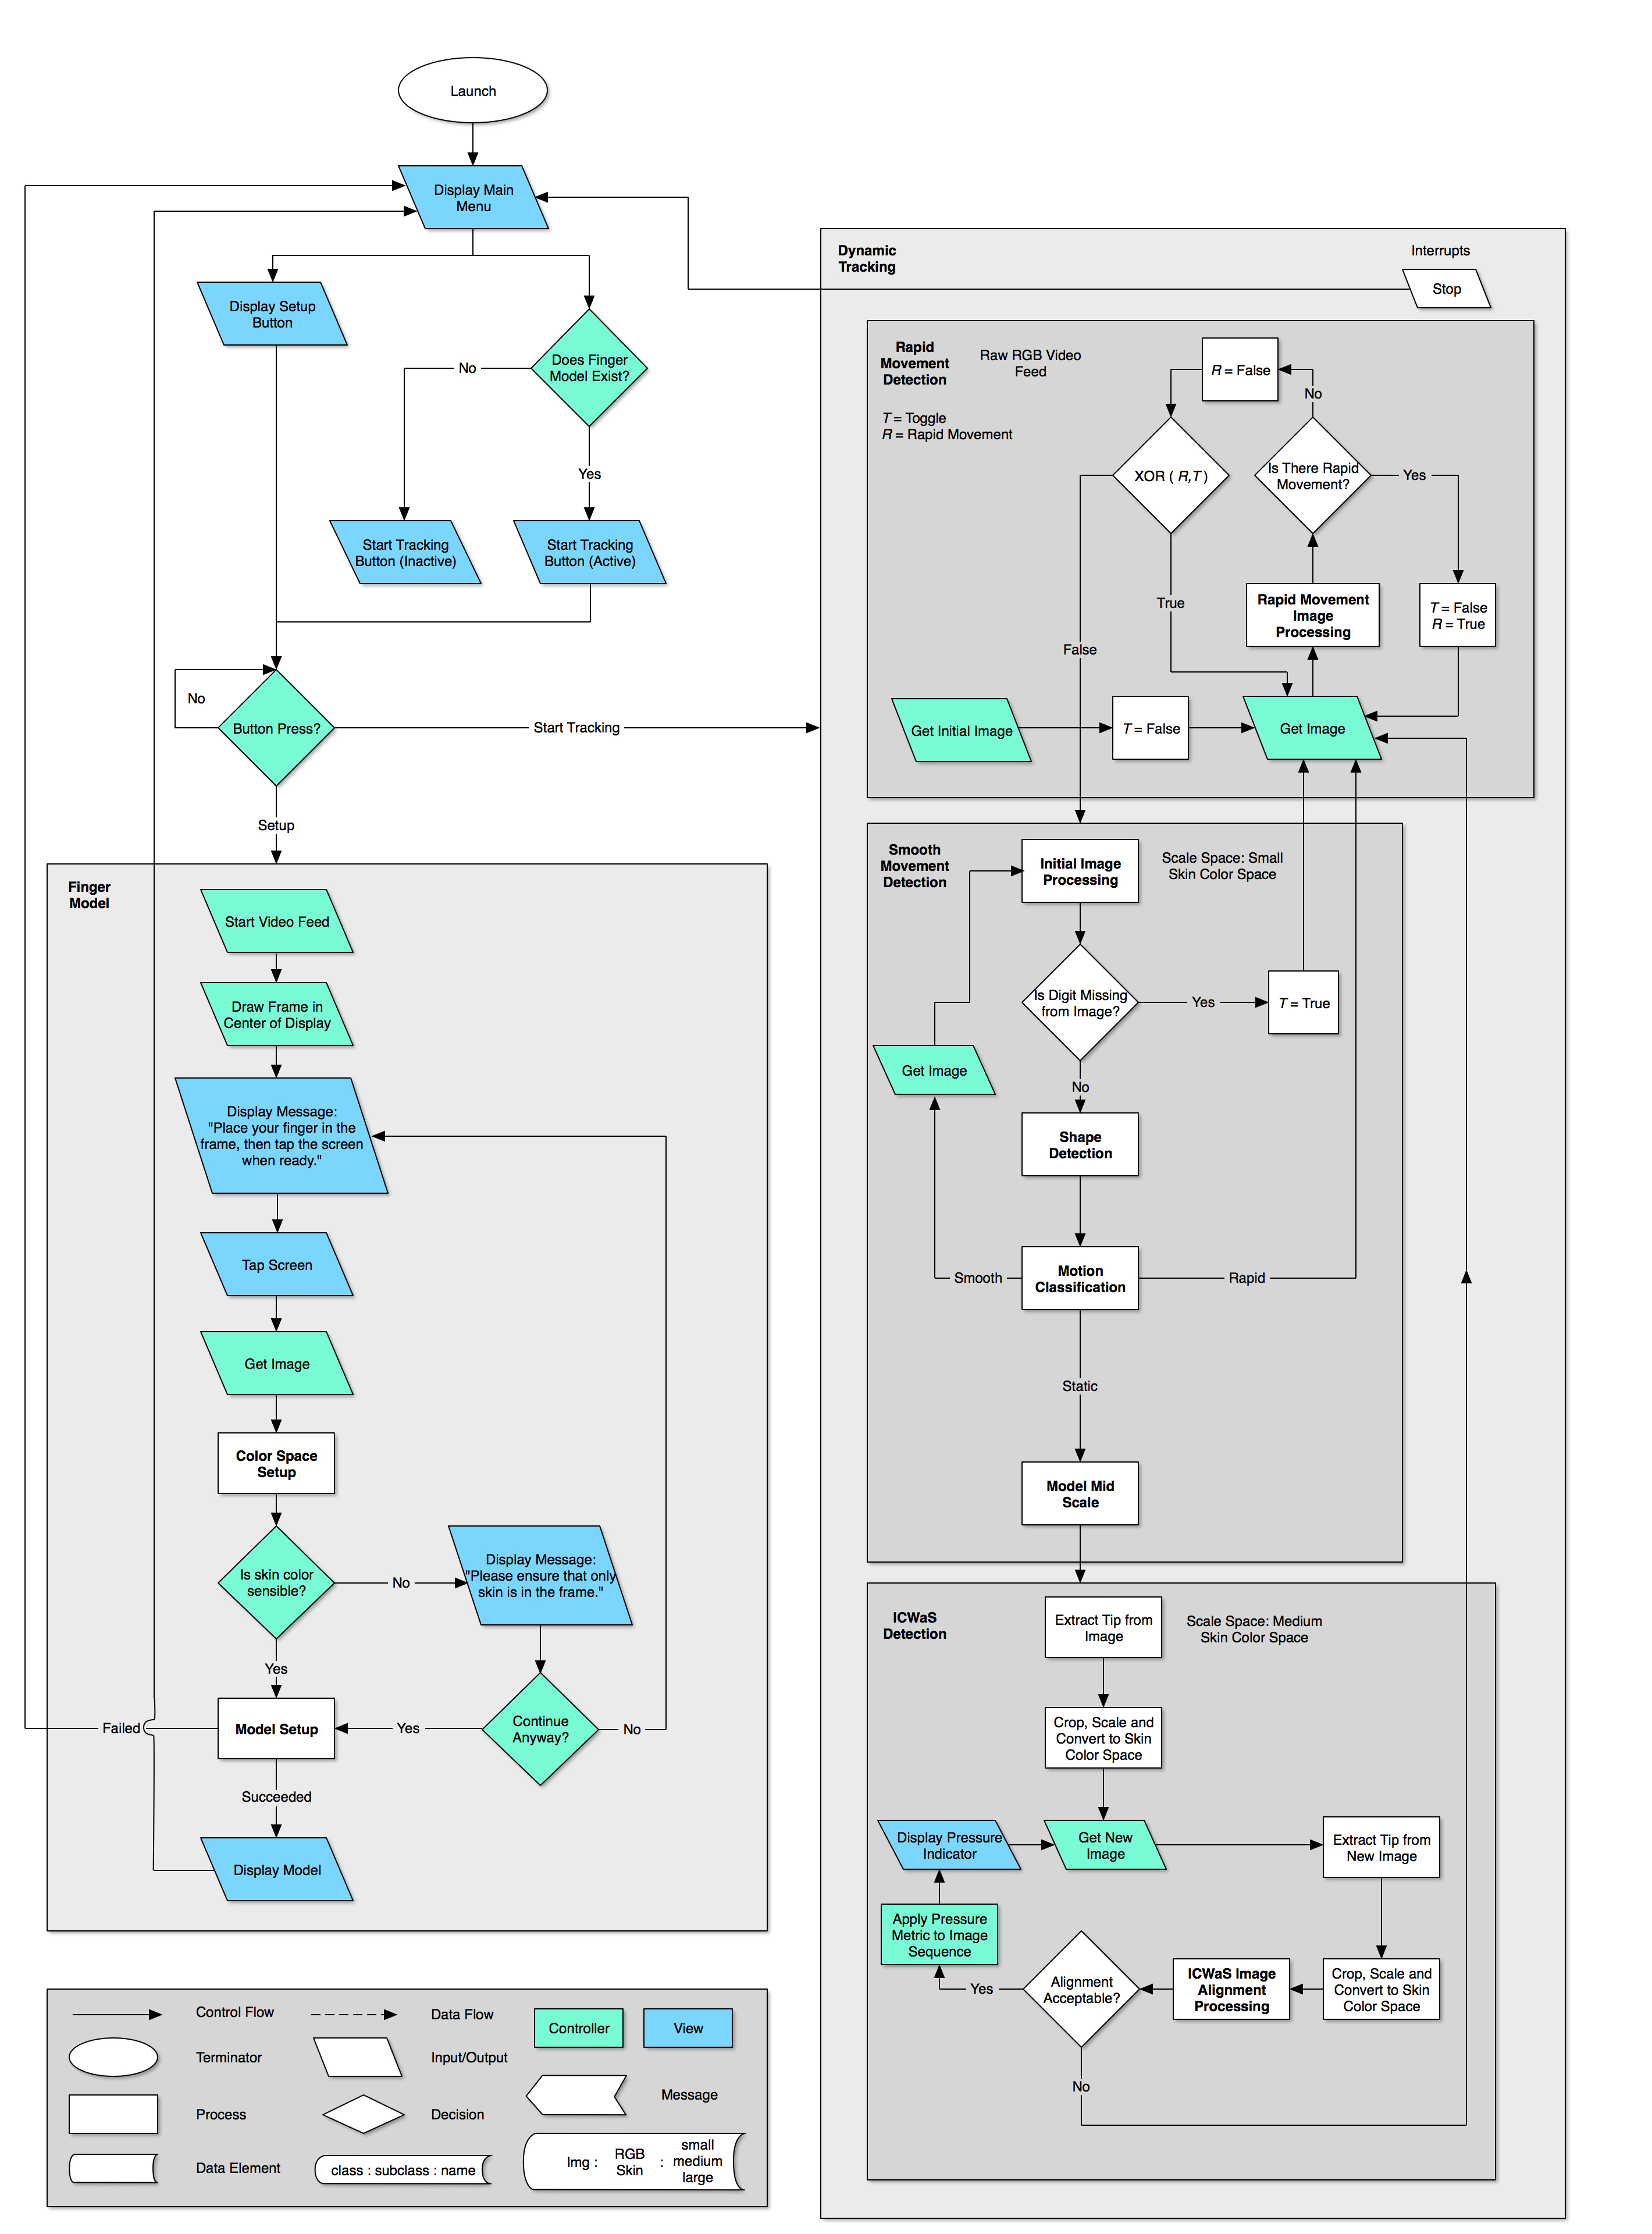
\includegraphics[width=0.97\textwidth]{Chapter4/Figs/Fingerpress_UI.jpg}
    \caption{Fingerpress UI flowchart}\label{fig:FingerpressUI}
\end{figure}

The chart \ref{fig:FingerpressUI} fails to address how the model, controller and view are each running in their own threads, and so control never actually passes from the model to the controller, or vice versa. So, in the MVC structure, the model and the view may only message the controller to indicate that an event has happened. For instance, when processing a video stream, if every time the dynamic tracking part of the model required a new image, a request message must be sent to the controller, then it would need to wait for the controller to get the image from the video stream and send it to the model, i.e. the model would often be waiting for the controller to respond. For this reason, in practice, the model uses OpenCV's video stream handling capabilities to get an image directly from the video stream.

\begin{figure}[h!]
  \centering
    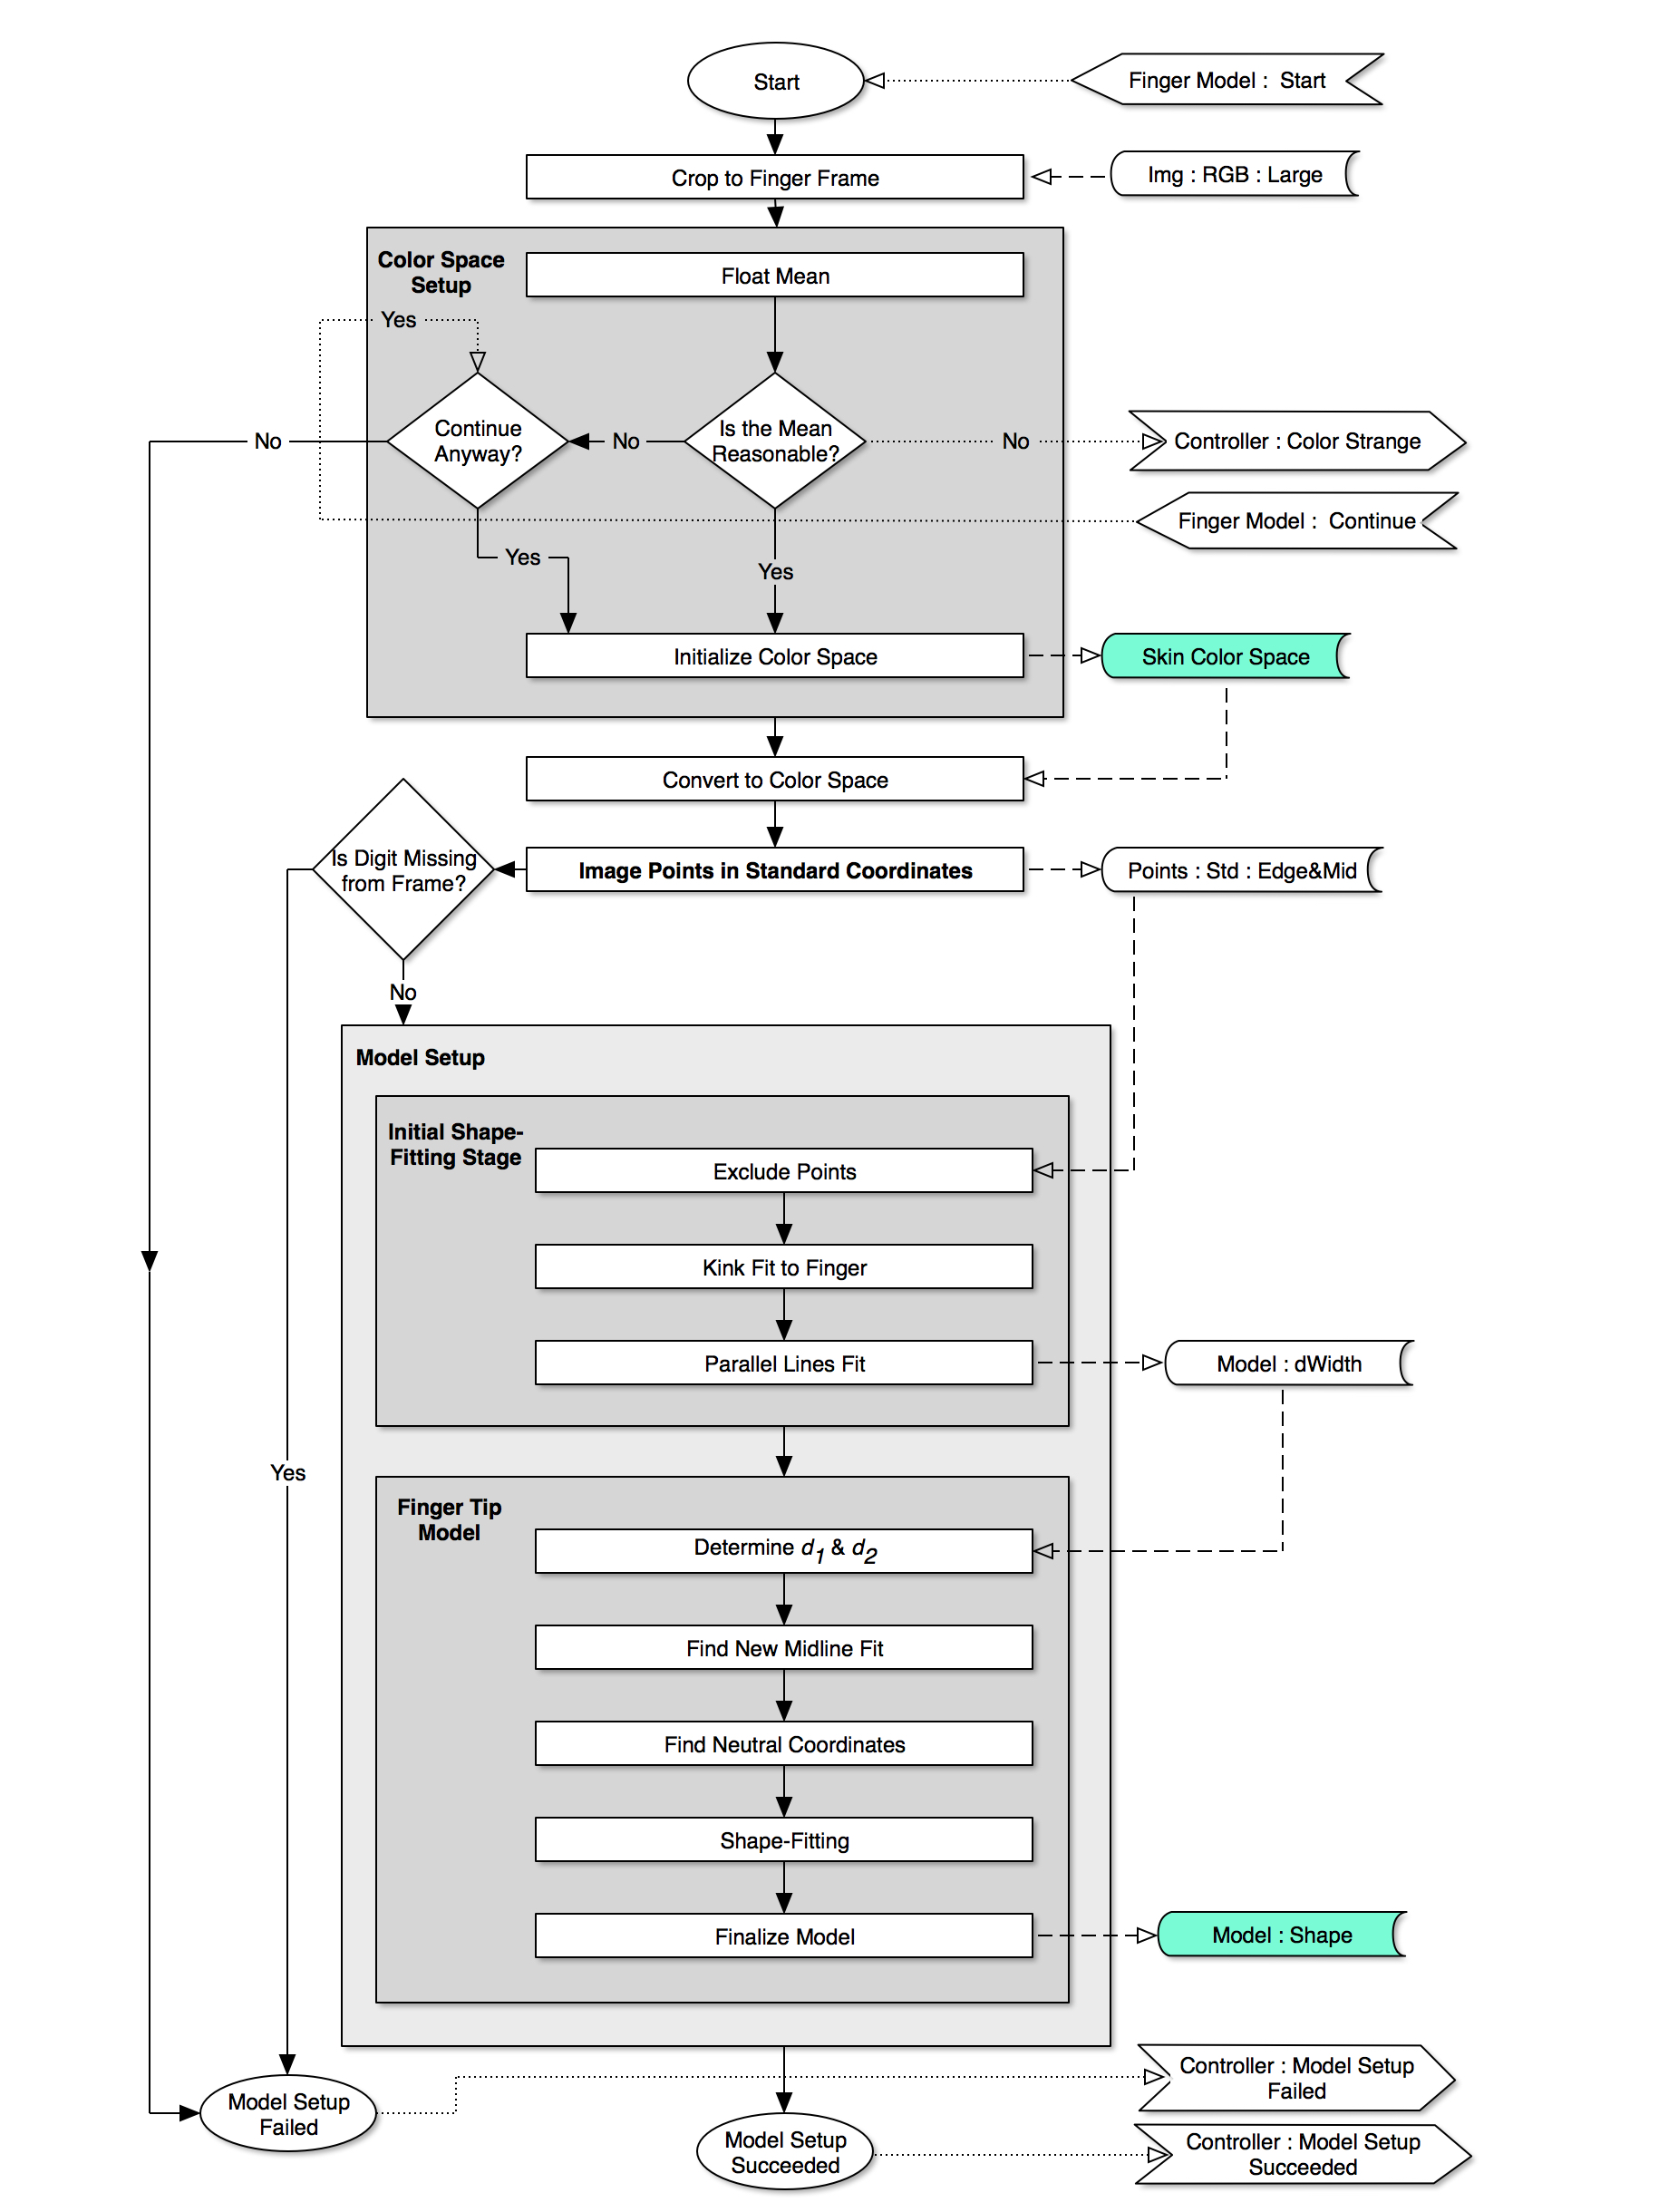
\includegraphics[width=0.95\textwidth]{Chapter4/Figs/Fingerpress_Finger_Model.jpg}
    \caption{Finger model flowchart}\label{fig:FingerpressFingerModel}
\end{figure}

\begin{figure}[h!]
  \centering
    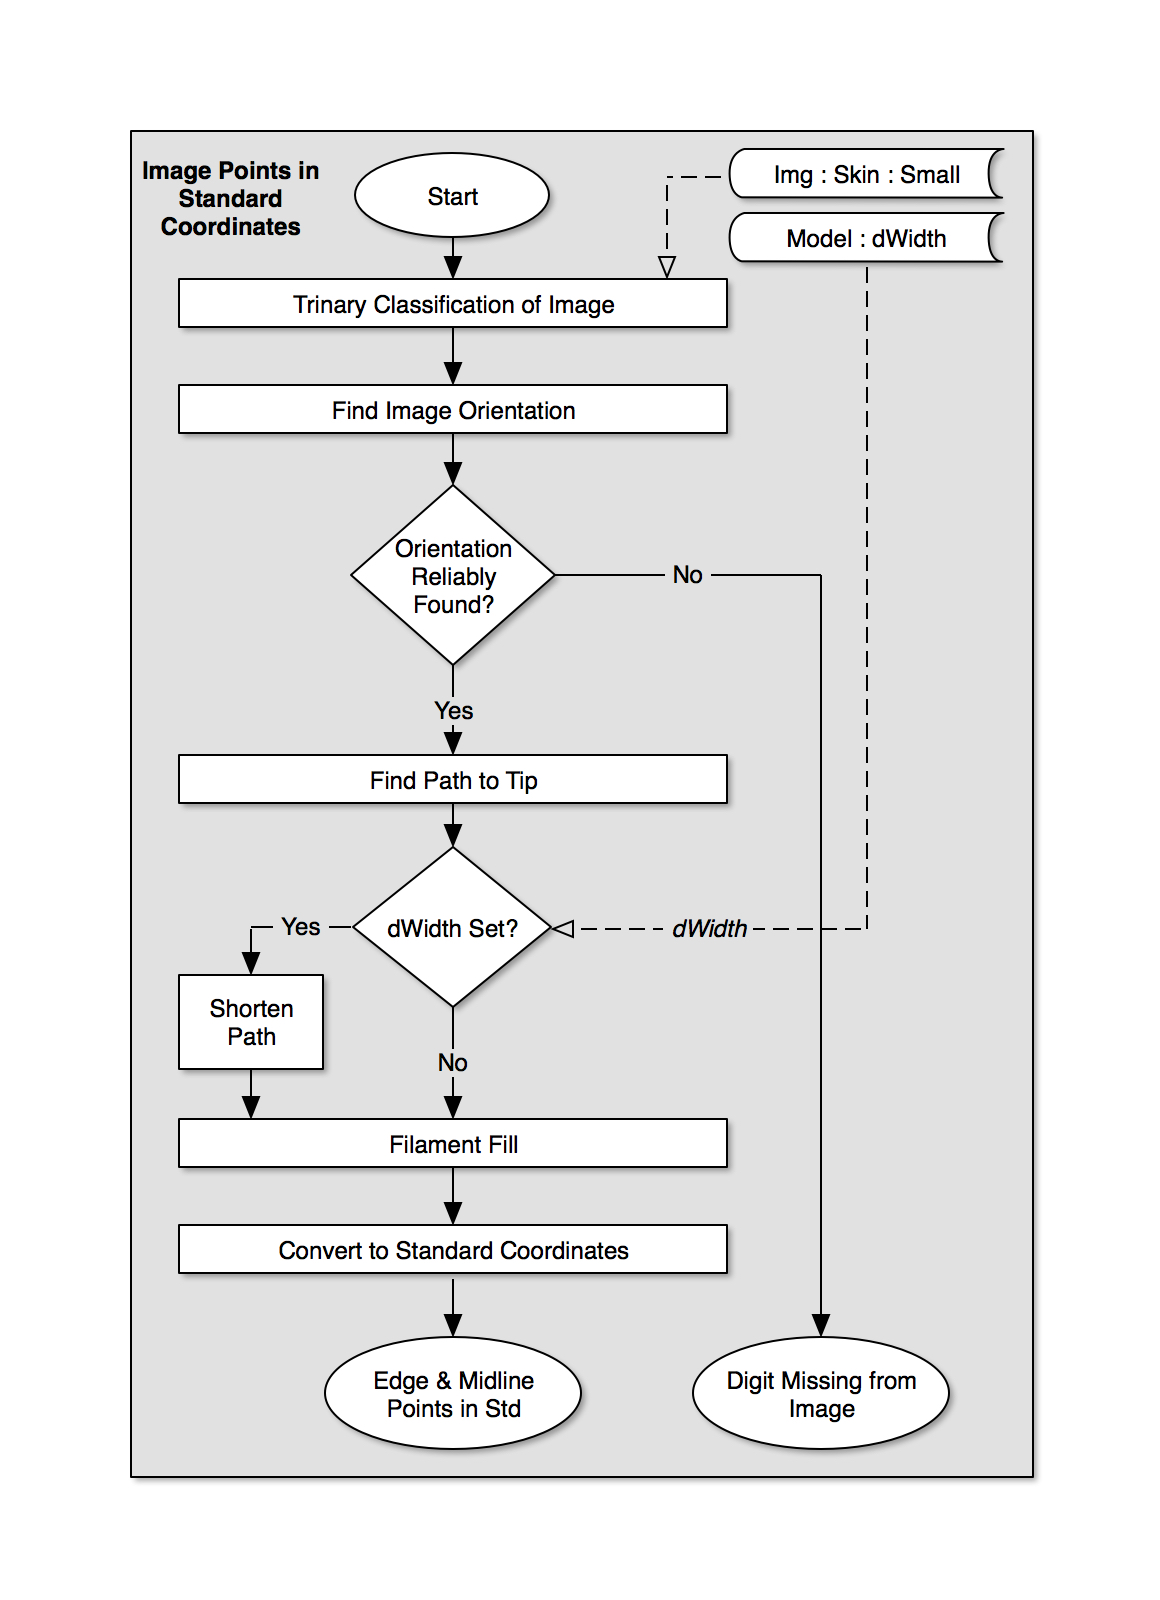
\includegraphics[width=0.49\textwidth]{Chapter4/Figs/Fingerpress_Std_Coordinates.jpg}
    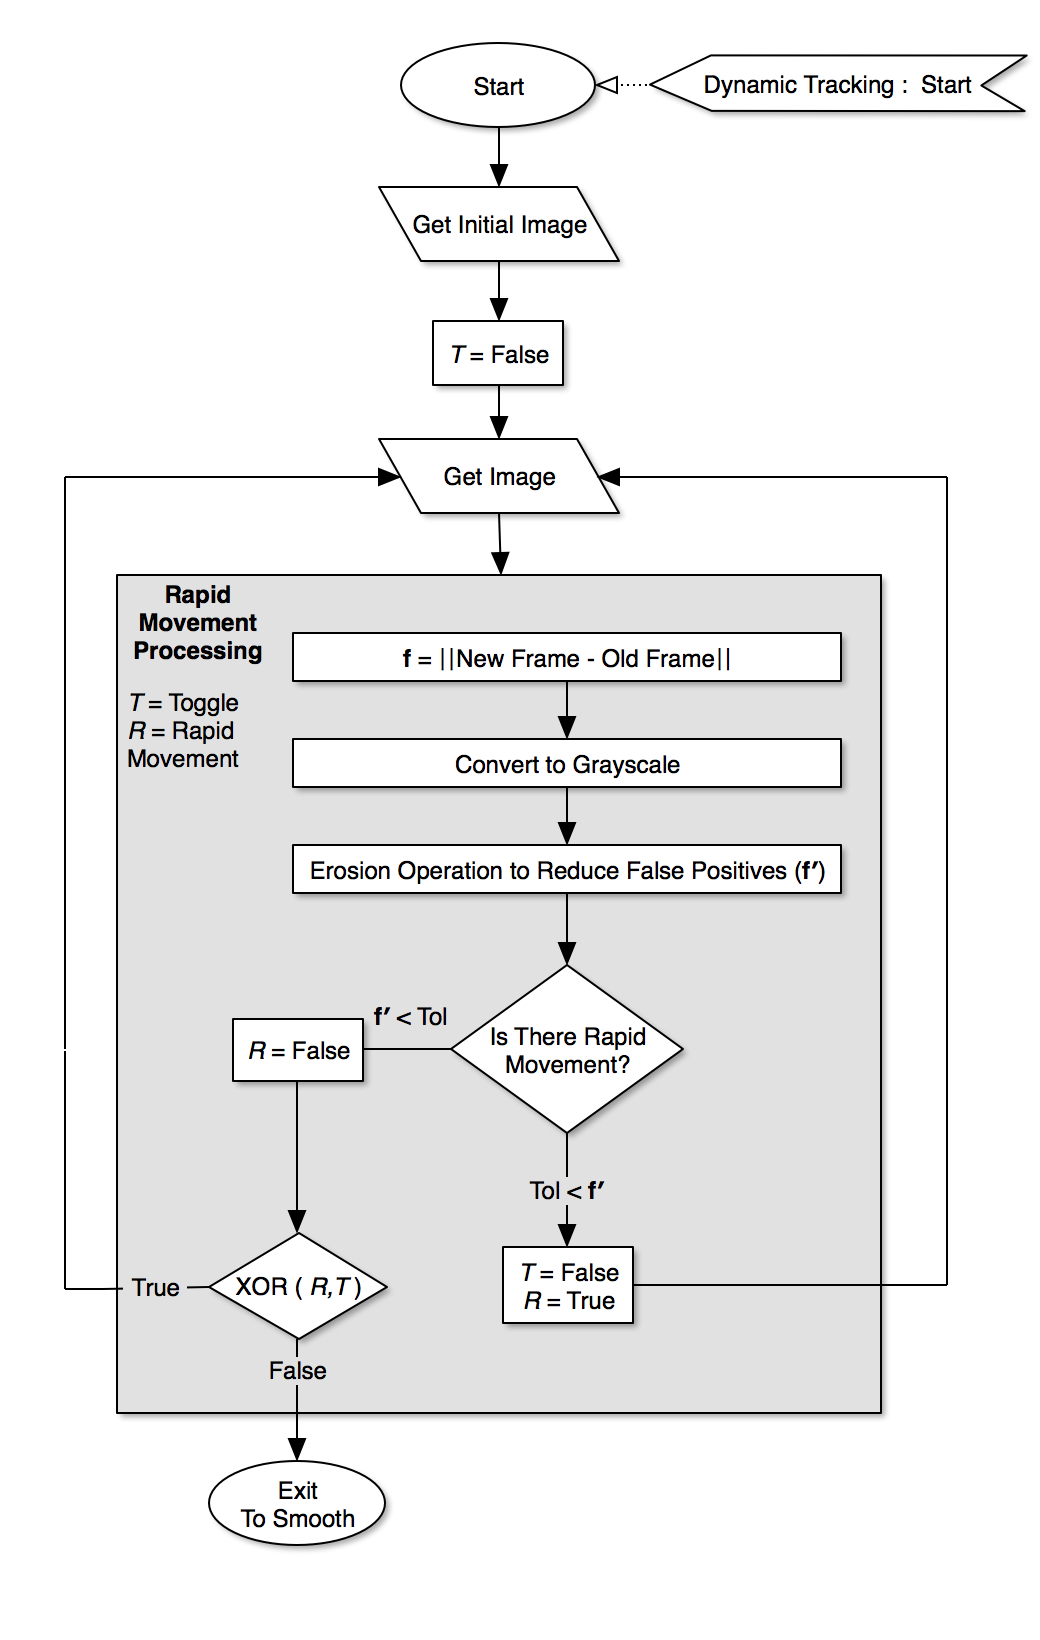
\includegraphics[width=0.49\textwidth]{Chapter4/Figs/Fingerpress_Rapid_Movement.jpg}
    \caption{Flowcharts for finding image points in standard coordinates (left), and rapid motion detection (right).}\label{fig:FingerpressStdCoordinates&RapidMovement}
\end{figure}

\begin{figure}[h!]
  \centering
    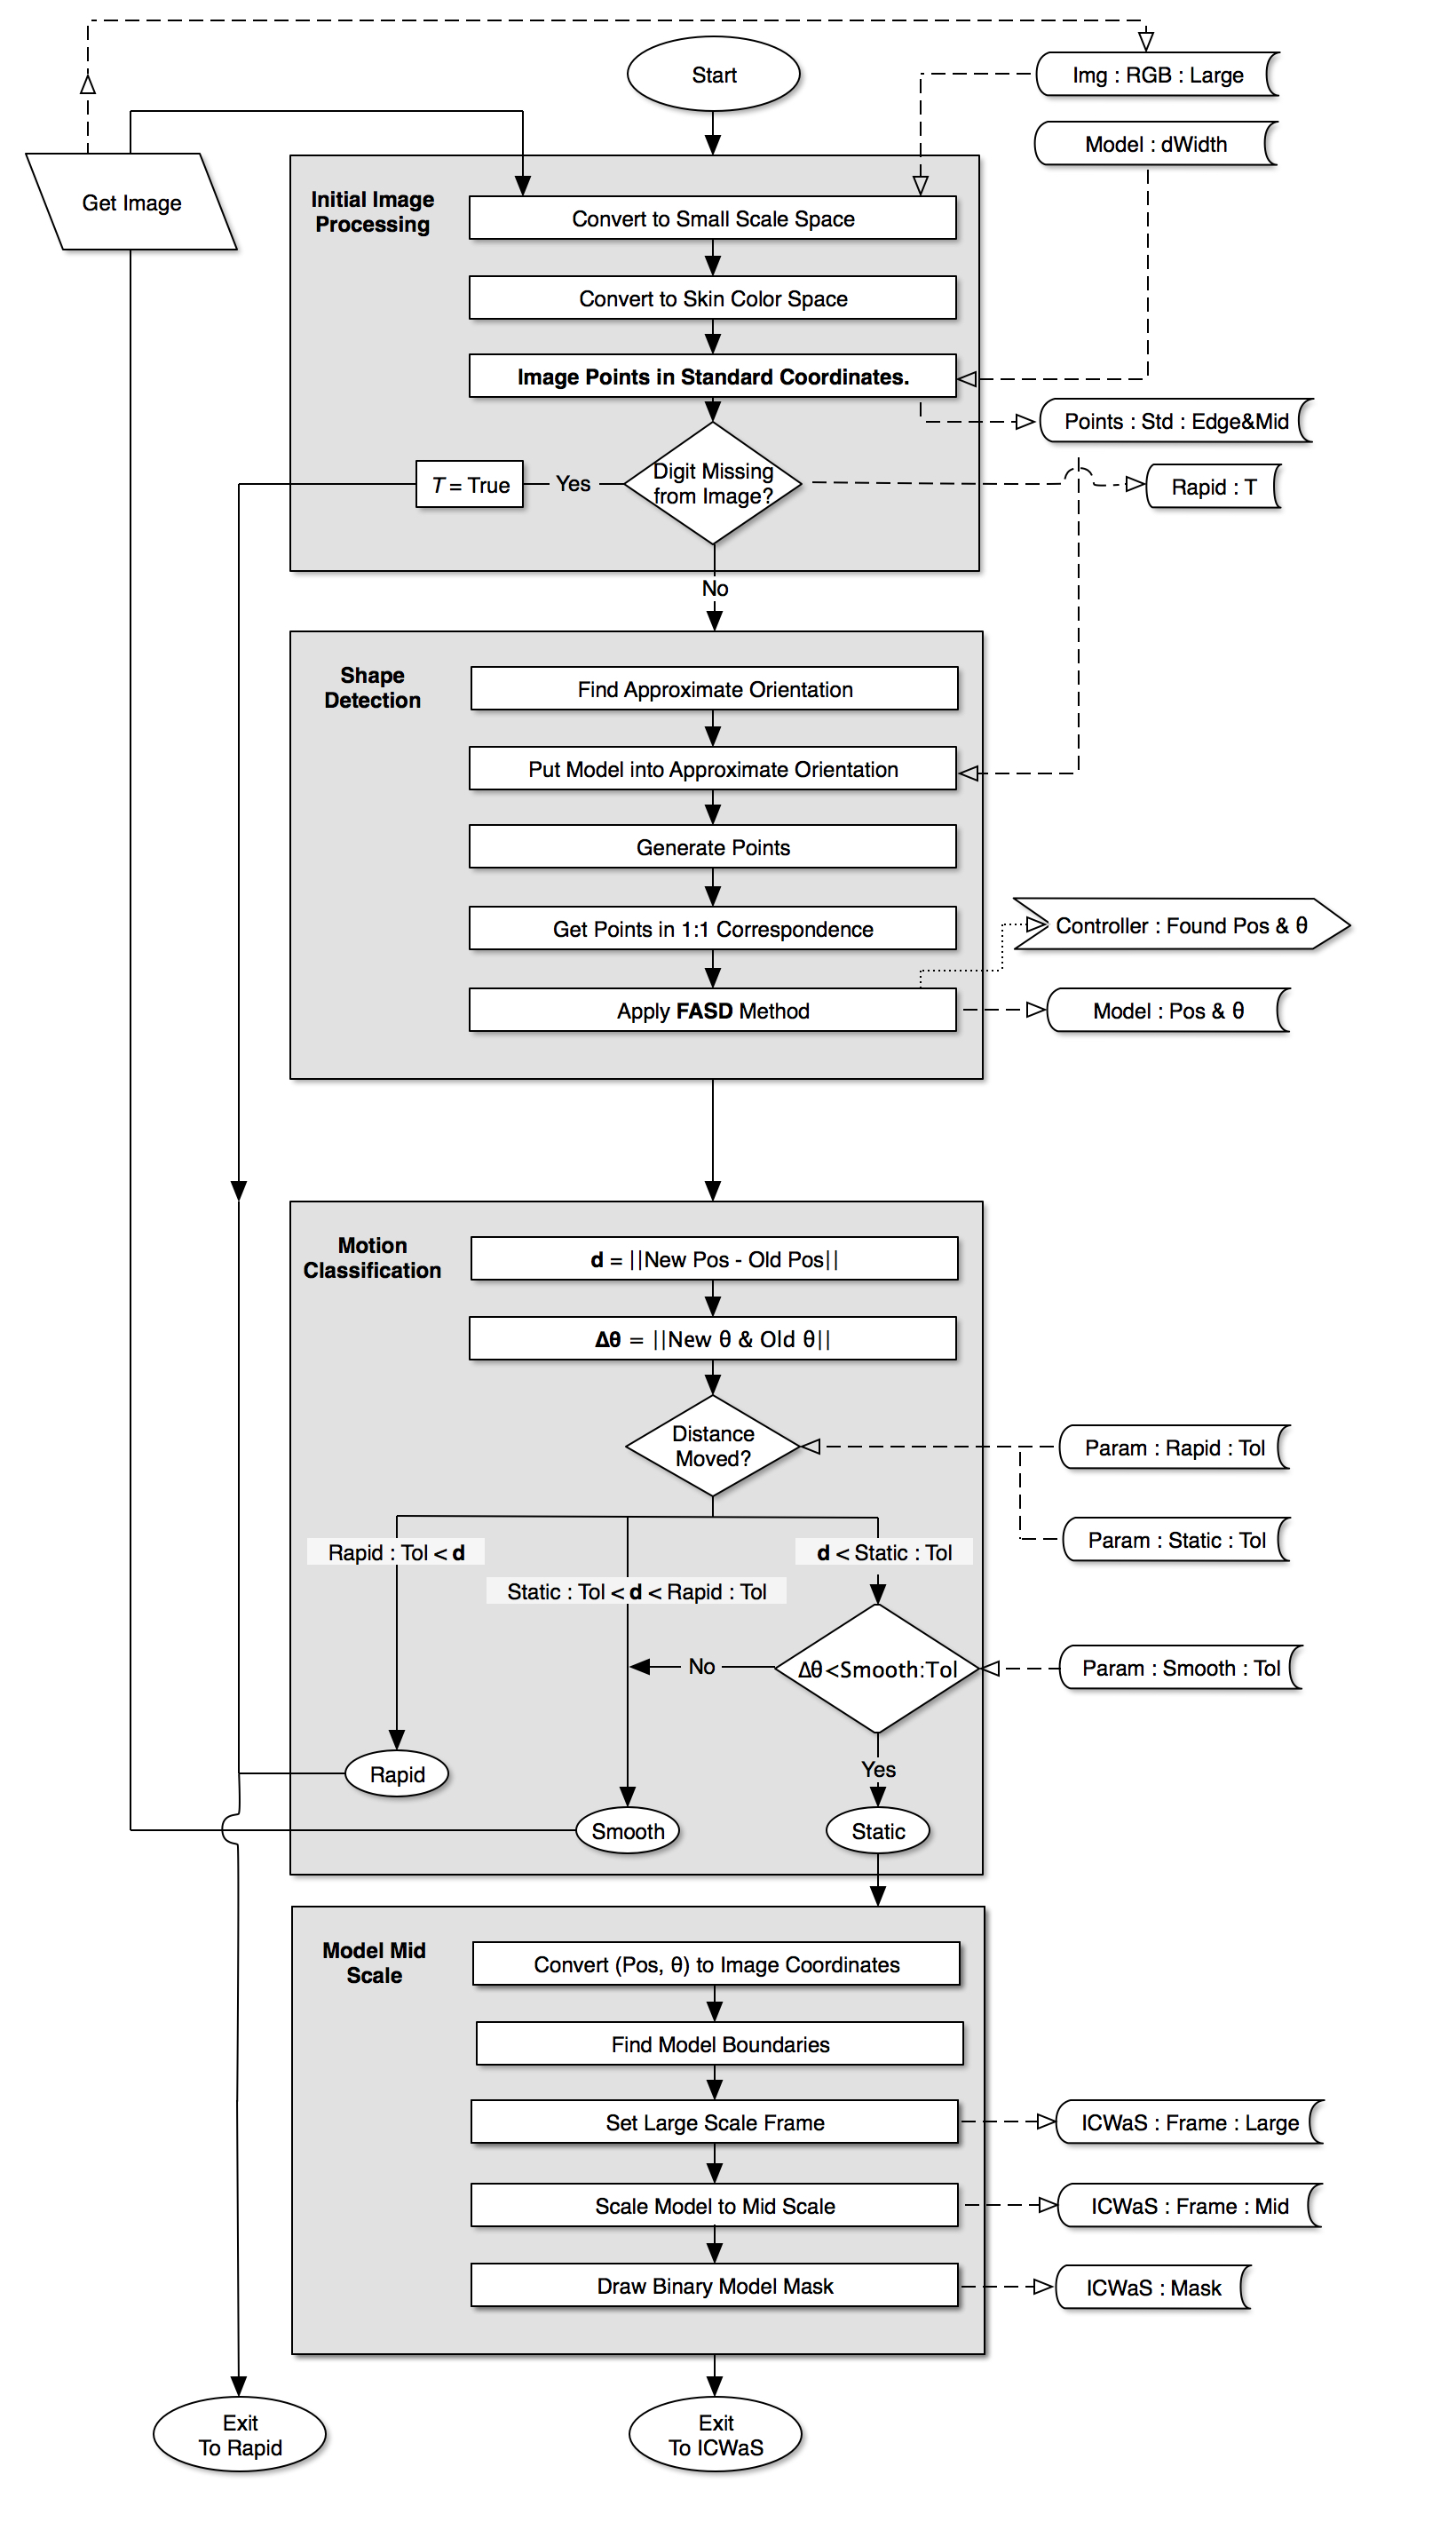
\includegraphics[width=0.90\textwidth]{Chapter4/Figs/Fingerpress_Smooth_Movement.jpg}
    \caption{Smooth movement flowchart}\label{fig:FingerpressSmoothMovement}
\end{figure}

\begin{figure}[h!]
  \centering
    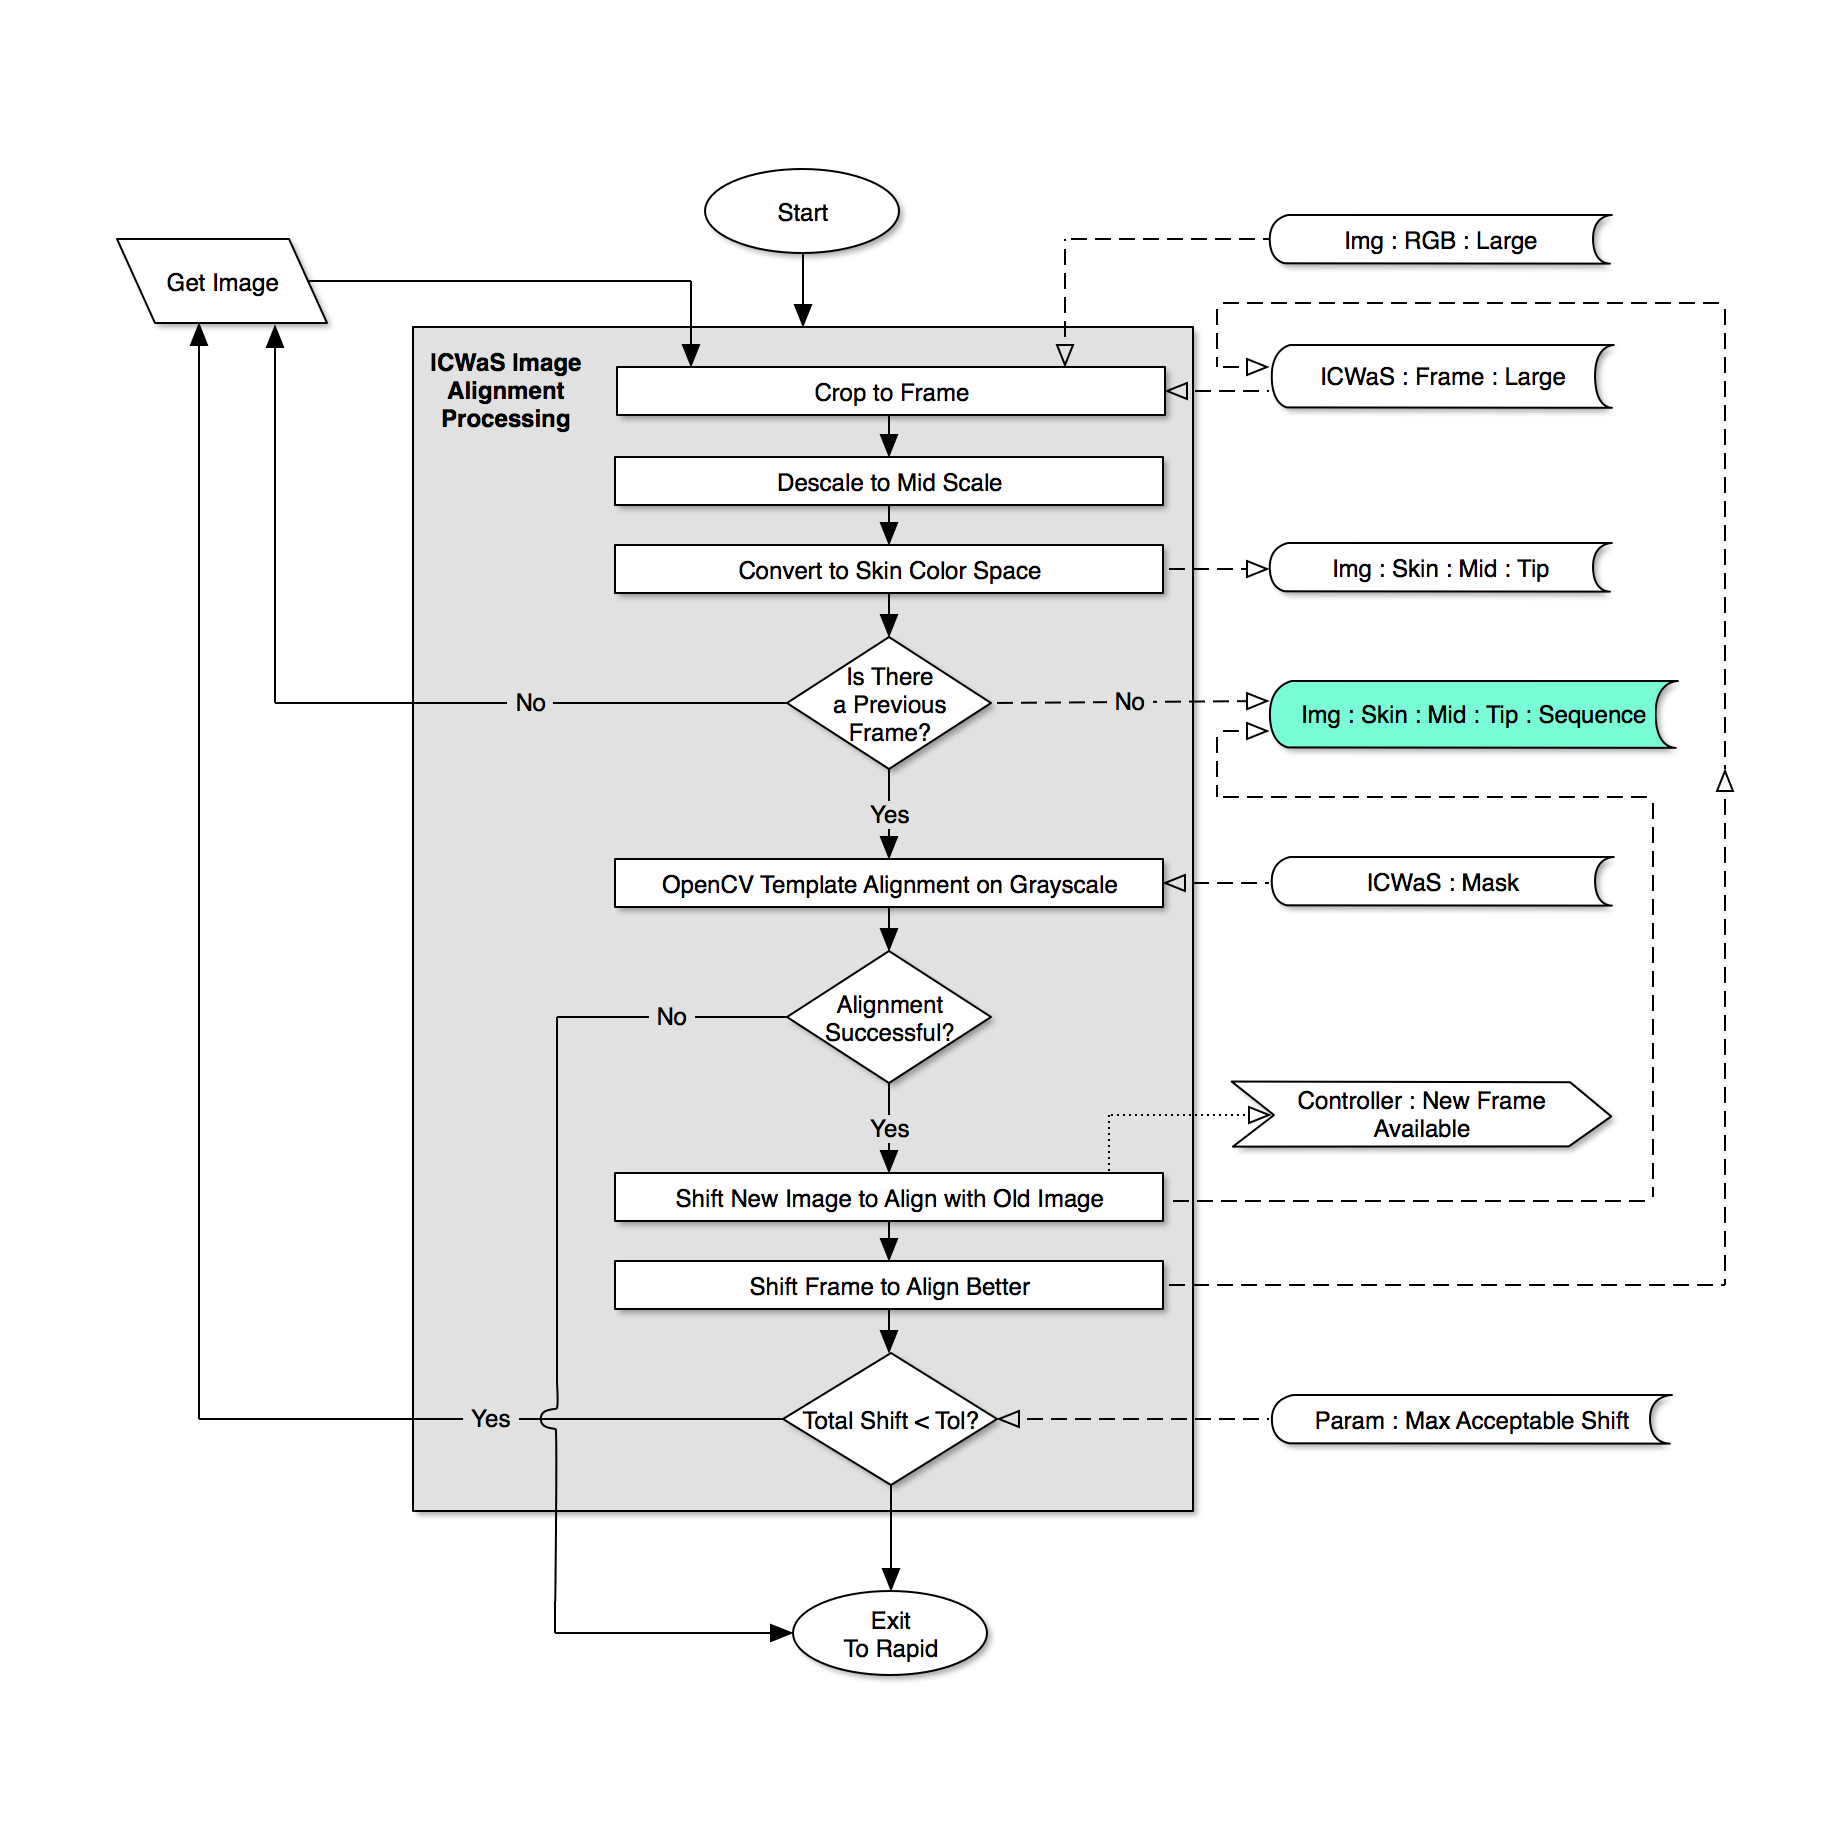
\includegraphics[width=0.95\textwidth]{Chapter4/Figs/Fingerpress_ICWaS.jpg}
    \caption{ICWaS flowchart}\label{fig:FingerpressICWaS}
\end{figure}

The charts in Figures \ref{fig:FingerpressFingerModel}, \ref{fig:FingerpressStdCoordinates&RapidMovement}, \ref{fig:FingerpressSmoothMovement} and \ref{fig:FingerpressICWaS} more accurately depict the actual implementation of the model by showing the data flow to the elements of the model which are accessible to the controller. 
\clearpage

